\documentclass[openright,twoside,10pt]{book}
\usepackage[b5paper,left=2cm,top=2.5cm,right=1.5cm,bottom=2.5cm]{geometry} 
\usepackage[spanish]{babel} % espanol
\usepackage[utf8]{inputenc} % acentos sin codigo
\usepackage{graphicx} % gráficos
\usepackage{lscape}
\usepackage{fancyvrb}
\usepackage{fancyhdr}
\usepackage{wrapfig}
\usepackage{multirow}
\usepackage{rotating} % rotate figures
\usepackage{array} % for defining a new column type
\usepackage{varwidth} % for the varwidth minipage environment
\newcolumntype{S}{>{\begin{varwidth}{2cm}}c<{\end{varwidth}}}
\newcolumntype{M}{>{\begin{varwidth}{4cm}}c<{\end{varwidth}}}
\newcolumntype{L}{>{\begin{varwidth}{6cm}}c<{\end{varwidth}}}
\newcolumntype{X}{>{\begin{varwidth}{8cm}}c<{\end{varwidth}}}
\newcolumntype{Y}{>{\begin{varwidth}{10cm}}l<{\end{varwidth}}}
\usepackage{float}
\usepackage{listings} %% START: Definimos el modo de mostrar codigo
\usepackage{color}
%\usepackage{bera}% optional: just to have a nice mono-spaced font
\usepackage{xcolor}
\usepackage{enumitem}
\usepackage[table,xcdraw]{xcolor}
\colorlet{punct}{red!60!black}
\definecolor{background}{HTML}{EEEEEE}
\definecolor{delim}{RGB}{20,105,176}
\colorlet{numb}{magenta!60!black}
\definecolor{dkgreen}{rgb}{0,0.6,0}
\definecolor{gray}{rgb}{0.5,0.5,0.5}
\definecolor{mauve}{rgb}{0.58,0,0.82}
\lstset{frame=tb, % VIM
  language=java,
  aboveskip=3mm,
  belowskip=3mm,
  showstringspaces=false,
  columns=flexible,
  basicstyle={\small\ttfamily},
  numbers=none,
  numberstyle=\tiny\color{gray},
  keywordstyle=\color{blue},
  commentstyle=\color{dkgreen},
  stringstyle=\color{mauve},
  breaklines=true,
  breakatwhitespace=true,
  tabsize=2
}
\lstdefinelanguage{json}{ % Define JSON
    basicstyle=\normalfont\ttfamily,
    numbers=left,
    numberstyle=\scriptsize,
    stepnumber=1,
    numbersep=8pt,
    showstringspaces=false,
    breaklines=true,
    frame=lines,
    backgroundcolor=\color{background},
    literate=
     *{0}{{{\color{numb}0}}}{1}
      {1}{{{\color{numb}1}}}{1}
      {2}{{{\color{numb}2}}}{1}
      {3}{{{\color{numb}3}}}{1}
      {4}{{{\color{numb}4}}}{1}
      {5}{{{\color{numb}5}}}{1}
      {6}{{{\color{numb}6}}}{1}
      {7}{{{\color{numb}7}}}{1}
      {8}{{{\color{numb}8}}}{1}
      {9}{{{\color{numb}9}}}{1}
      {:}{{{\color{punct}{:}}}}{1}
      {,}{{{\color{punct}{,}}}}{1}
      {\{}{{{\color{delim}{\{}}}}{1}
      {\}}{{{\color{delim}{\}}}}}{1}
      {[}{{{\color{delim}{[}}}}{1}
      {]}{{{\color{delim}{]}}}}{1},
}

\usepackage[table,xcdraw]{xcolor} % tabla con colores
\setlength{\parskip}{10pt plus 1pt minus 1pt}
 % aqui definimos el encabezado de las paginas pares e impares.
\rhead[]{}

\renewcommand{\headrulewidth}{0.5pt}

% aqui definimos el pie de pagina de las paginas pares e impares.
\rfoot[\thepage]{\thepage}
\cfoot[]{}
\renewcommand{\footrulewidth}{0pt}

% Arreglamos el problema de 'Indice de cuadros' por 'Índice de Tablas'
% \renewcommand{\listoftables}{Índice de Tablas}

% aqui definimos el encabezado y pie de pagina de la pagina inicial de un capitulo.
\fancypagestyle{plain}{
\fancyhead[R]{}
\fancyfoot[C]{}
\fancyfoot[R]{\thepage}
\renewcommand{\headrulewidth}{0.5pt}
\renewcommand{\footrulewidth}{0pt}
}

\pagestyle{fancy} % seleccionamos un estilo

\date{21 de Enero de 2020}
\author{Velasco Gil, Álvaro}
\title{TFG: titulo}

\begin{document}

\begin{titlepage}

\begin{center}
\vspace*{-1in}
\begin{figure}[htb]
\begin{center}
\includegraphics[width=3cm]{./img/logo}
\end{center}
\end{figure}
\begin{large}
\textbf{Universidad de Valladolid}
\end{large}

\vspace*{0.15in}

\vspace*{0.6in}
\begin{large}
\textbf{ESCUELA DE INGENIERÍA INFORMÁTICA}

\end{large}
\vspace*{0.2in}
\textbf{ GRADO EN INGENIERÍA INFORMÁTICA}\\
\textbf{ MENCIÓN EN INGENIERÍA DEL SOFTWARE }
\vspace*{0.1in}
\rule{140mm}{0.1mm}\\
\vspace*{0.2in}
\begin{large}
\textbf{{\LARGE DISEÑO E IMPLEMENTACIÓN DE UN SISTEMA DE CONTROL Y MONITORIZACIÓN DE ASISTENTES INTELIGENTES\\}}
\end{large}
\vspace*{0.2in}
\rule{140mm}{0.1mm}\\
\vspace*{2in}
\begin{large}
\begin{flushright}
\textbf{Alumno: Álvaro Velasco Gil \\
\vspace*{0.3in}
Tutor: Jesús M. Vegas Hernández }
\end{flushright}
\end{large}
\end{center}

\end{titlepage}

\newpage
\mbox{}	
\thispagestyle{empty} % para que no se numere esta página

\chapter*{}
\pagenumbering{Roman} % para comenzar la numeración de paginas en números romanos
\begin{flushright}
\textit{%Dedicatoria,\\
Dedicado a mis padres y mi hermana, por confiar en mi cuando yo no lo hacía.}
\end{flushright}


\chapter*{Agradecimientos} % si no queremos que añada la palabra "Capitulo"
\addcontentsline{toc}{chapter}{Agradecimientos} % si queremos que aparezca en el índice
\markboth{AGRADECIMIENTOS}{AGRADECIMIENTOS} % encabezado 
Quiero agradecer en primer lugar a mi tutor, por la paciencia,

a mis amigo Jorge Sanz por facilitarme los primeros cursos,

a Javier Helguera por hacerme la carrera más llevadera,

a Diego Dominguez y David Escarda por hacer más sencillas las noches estudiando en el aulario,

y a mi familia, por soportar mis cambios de humor.
% Aquí agradecer

\chapter*{Resumen} % si no queremos que añada la palabra "Capitulo"
\addcontentsline{toc}{chapter}{Resumen} % si queremos que aparezca en el índice
\markboth{RESUMEN}{RESUMEN} % encabezado
\begin{flushleft}

Este proyecto se basa en dos grandes motivaciones: la privacidad, y la asistencia de la población envejecida rural.

Con ello, se narra el proceso por el cual ha sido desarollado un proyecto de despliegue de dispositivos, los cuales se comportan como asistentes personales orientados a la población más envejecida y con menos recursos, que notablemente está alojada en poblaciones rurales.

Estos asistentes proporcionarán una ayuda diaria a este grupo social que es el que en realidad puede necesitar de un dispositivo que le ayude a realizar las tareas y responder preguntas comunes, al igual que se tratará de un dispositivo que pueda detectar un posible accidente en el hogar y proporcionar una asistencia inmediata.

Para la realización de este proyecto, por tanto, se requiere la implementación de una API contra la que se comunicará cada dispositivo, al igual que un sitio web para que el administrador del sistema pueda controlarlos. Cada dispositivo estará desplegado remotamente y podrá ser controlado, por lo que en este proyecto también se desarrollará el controlador del dispositivo.

En cuanto al desarrollo se han utilizado diferentes lenguajes, tales como Kotlin con el framework de Ktor para la creación de la API, el framework de VueJS para la creación del sitio web, donde se incluye HTML + CSS + Javascript, al igual que la utilización de Phyton para la creación del controlador que irá instalado en cada dispositivo.

Toda el proyecto ha sido elaborado, dada su naturaleza, siguiendo un plan basado en iteraciones.

% Aquí el resumen

\end{flushleft}

\chapter*{Abstract} % si no queremos que añada la palabra "Capitulo"
\addcontentsline{toc}{chapter}{Abstract} % si queremos que aparezca en el índice
\markboth{ABSTRACT}{ABSTRACT} % encabezado
\begin{flushleft}

% Aquí va el abstract

\end{flushleft}

\tableofcontents % indice de contenidos

\cleardoublepage
\addcontentsline{toc}{chapter}{Lista de Figuras} % para que aparezca en el indice de contenidos
\listoffigures % indice de figuras

\cleardoublepage
\addcontentsline{toc}{chapter}{Lista de Tablas} % para que aparezca en el indice de contenidos

%lista de tablas
\renewcommand\listtablename{Índice de Tablas}
\listoftables % indice de tablas
\clearpage

\chapter{Introducción}\label{cap.introduccion}
\pagenumbering{arabic} % para empezar la numeración con números
\section{Introducción}

En este proyecto se abordará el proceso de control y monitorización remota de dispositivos asistentes inteligentes.

Tras la lectura de este documento se comprenderán tanto los motivos por los cuales se ha decidido tomar esta opción, como el proceso de despliegue del sistema, pasando por las fases de implementación en las que se enseñará a replicar proyectos de estructura similar, como por las fases de desarrollo en la cuales se estudian los posibles riesgos y características del proyecto, al igual que por el plan de desarrollo en el cual se programa toda la elaboración.

\section{Motivación}

La idea de este proyecto llegó impulsada gracias a dos grandes motivaciones: conseguir la privacidad en la utilización de dispositivos inteligentes, y la posibilidad de asistir a la población envejecida de entornos rurales.

La primera motivación, relativa a la privacidad viene dada ya que los asistentes inteligentes están en auge y las grandes empresas están dando acceso a estos servicios de manera gratuita, donde lo único que hay que hacer para disfrutar de uno de ellos es pagar es el dispositivo físico, asumiendo únicamente los costes del hardware a un precio reducido, lo que hace cuestionar la idea del modelo de negocio que están siguiendo para que salga rentable: El desarrollo de un sistema software capaz de dar respuesta a toda cuestión que un usuario se llegue a plantear, al igual que el mantenimiento de las infraestructuras que puedan soportar todo un sistema capaz de retroalimentarse mediante la información vertida por los usuarios, tiene un coste muy elevado como para ofrecer ese servicio de manera gratuita. Un modelo de negocio en el cual  se ofrece un dispositivo a un bajo precio con unas prestaciones de gran nivel sin cobrar a mayores una cuota mensual da que pensar, por ejemplo, que el producto mediante el cual está basado su modelo de negocio no es el que el usuario cree: Para el usuario, el producto es el dispositivo que le va a servir un uso, pero para la empresa, el producto es toda la información personal que le va a proporcionar cada usuario que utilice el dispositivo. La información recopilada a través de los asistentes, al ser obtenida directamente de los hogares de cada usuario no es solamente privada, si no que también es íntima, lo que hace cuestionarse si realmente la comunidad de usuarios sabe que hay empresas aprovechándose de las conversaciones de su día a día para recolectar toda la información de un usuario que fluye en los lugares más personales de cada hogar, capturando información con gran potencial, ya sea sobre gustos, tendencias, necesidades o inclinaciones políticas, con el fin de poder no solo utilizar esos datos, sino también pudiendo incluso venderlos a terceros, a través de los cuales pueden llegar a intentar manipularnos, como ya se ha visto en casos como el escándalo de Cambridge Analytica.~\cite{cambridge} 

Esta aparente ignorancia de la población sobre el tratamiento de datos que las empresas podrían ser capaces de hacer genera la motivación suficiente para la creación de un nuevo dispositivo asistente, el cual haga más fácil la vida de un sesgo de la sociedad al cual iría orientado, sin tener la necesidad ni posibilidad de almacenar datos de carácter sensible.

Por otro lado también se observa otra gran motivación para la elaboración del proyecto, y es producida por la migración por la parte joven de la sociedad en los tiempos que acontecen actualmente, lo cual está provocando una despoblación en sus lugares de origen, dejando a los familiares de mayor edad en soledad, siendo la parte de la familia que a grosso modo necesita más atención y requiere más ayuda para pasar el día.

La implementación de un asistente inteligente el cual ayude a este conjunto de la sociedad a entretenerse proponiendo tanto eventos cercanos a ellos, como respondiendo sus dudas de una manera rápida, o sirviéndoles para buscar ayuda en caso de posible caída o solicitud de auxilio, puede ser una gran herramienta que mejore su calidad de vida.


\section{Objetivos}

Dadas y mencionadas las motivaciones que impulsan este proyecto, se puede destacar que el objetivo principal se basa en la privacidad por diseño.

El objetivo de este proyecto se logrará, por tanto, mediante el despliegue de un sistema que permita la conexión de dispositivos al servidor de manera automática y remota, a la vez que permita que sean controlados desde un sitio web de administración de una manera simple, desde la cual se podrá ver también estadísticas de uso para poder comprobar el estado de los usuarios, sin la obtención de datos que atenten contra su privacidad.

Estos dispositivos, como objetivo, estarán orientados a personas del rango de la tercera edad, estando cada dispositivo asignado a una persona, de la cual se conoce su localidad con el fin de obtener información relacionada a la hora de responder.

Los dispositivos podrán entonces ser controlados remotamente por parte de los administradores y podrán ser configurados tanto de manera individual, como en función de su localidad, o de una manera global, pudiendo solicitar al dispositivo la actualización de manera remota a través de configuraciones, o solicitar la realización de diferentes acciones como puede ser la auto-configuración de la red Wi-Fi, u otras para mejorar la gestión de despliegue sin requerir la conexión física con un ordenador.




\chapter{Estado del Arte}\label{cap.arte}
\section{Introducción}
\subsubsection{Preámbulo}

Los asistentes virtuales cada vez están más presentes en nuestras vidas gracias a todos los avances de la tecnología, y puede verse en que ya aparecen en todos los teléfonos móviles para ayudar en el día a día de los usuarios, ya sea para responder preguntas, poner una canción, o buscar información de manera rápida para el usuario.

La utilización de estos asistentes virtuales hace que cada vez más personas se planteen la posibilidad de llevar más lejos la utilización de ellos, como puede ser a través de otros dispositivos inteligentes a los que se les está buscando hueco cada vez en más hogares.

Estos dispositivos nos hacen la vida más sencilla, ayudando a actualizar y controlar toda la domótica de nuestras casas, de manera que se puedan realizar acciones en nuestra vivienda que hace unos años solo se podían imaginar en películas de ciencia ficción.

La utilización de asistentes virtuales para facilitar acciones que se repiten de manera continuada a lo largo de los días está cada vez más de moda: según un estudio de la reputada Nielsen~\cite{nielsen}, durante el Q2 de 2018 ha llegado a crecer el número de dispositivos desplegados en los hogares de Estados Unidos hasta alcanzar el 24\% de la población.

A la pregunta de para qué puede querer el 24\% de las familias un dispositivo asistente en sus casas, se puede observar tras una encuesta de dicho estudio, que en la mayoría de hogares se daba un uso bastante simple, solicitando al dispositivo únicamente la reproducción de contenido multimedia, pero esto ocurre únicamente en las primeras semanas de uso. También se puede observar en el estudio que, posteriormente, se tiende a dar más uso al dispositivo llegándole a requerir información habitual que se requiere de manera repetitiva cada semana, como puede ser la consulta del tiempo, la del tráfico antes de ir a trabajar o a la consulta de algún evento cercano importante.

La simplicidad de uso y todas las posibilidades que abarca ha hecho que una vez ha sido usado este tipo de dispositivo inteligente en cualquier hogar, se le siga utilizando cada vez para más tareas, dada su usabilidad y abanico de utilidades.

En ese estudio arriba citado, también se puede observar el comportamiento de los usuarios: una vez el dispositivo está en entre las cuatro paredes de la casa, se tiende a acompañar a este dispositivo inteligente de otros dispositivos domóticos, convirtiendo poco a poco el hogar en un sistema interconectado: cuatro de cada diez hogares disponen de más de un dispositivo inteligente en el hogar, y el 45\% de los hogares se plantean acompañar al que ya tienen, comprando otro.

Esta gran aceptación a la domótica viene dada gracias a la cantidad de variantes de las cuales podemos dotar al hogar, pudiendo ser todas controladas a través del dispositivo asistente, así como puede ser la programación de los tiempos de uso de aparatos como las bombillas, el termostato, los sistemas de seguridad, e incluso tanto el frigorífico, el sistema de riego, u otras acciones relativas a la seguridad de la vivienda como puede ser bloquear las puertas y ventanas, al igual que mantener el registro de cuáles y cuándo han sido abiertas, entre otras muchas opciones.

Al irrumpir estos dispositivos en las acciones cotidianas de un día corriente, se le permite al usuario adaptarse y ver que estos aparatos le acaban facilitando el día.

Viendo el creciente uso de estos dispositivos y las grandes marcas que hacen acto de presencia facilitando su implementación, entre las cuales se encuentran Google o Amazon, se puede pensar que este mercado ya está dominado y pertenece a estos dos grandes imperios, pero en este caso no se va a tener en cuenta todo lo que ya ofrecen, sino que se va a tener en cuenta todo lo que no están ofreciendo, o qué es lo que sus dispositivos no están preparados para ofrecer:

Como bien se ha visto, el punto de mira en todo el tema de la domótica y asistentes tiene un público objetivo que es el que pertenece a un rango de edad al que le gusta la tecnología y le parecería interesante automatizar las tareas del hogar, pero el verdadero público que podría exprimir todo su potencial es el público que menos acostumbrado nos tiene a estar a la vanguardia de la tecnología, el público perteneciente a la tercera edad.

Si se realiza el acto de volver a pensar sobre lo que es un asistente personal, en cuanto a una persona que trabaja como asistente, se entiende que es una persona que ayuda en las acciones del día a día más simples y repetitivas para las que otra persona no es capaz de hacer por si misma por algún tipo de incapacidad, ya sea incapacidad temporal, o algún tipo de incapacidad física.

Una vez planteado a qué se dedica un asistente personal, es fácil darse cuenta que al hablar de este trabajador se plasme la imagen de una persona que ayuda a personas mayores, o a personas con algún tipo de discapacidad.

El rango de personas de tercera edad es un público que puede necesitar que le levanten las persianas de manera automática porque quizá, le cuesta levantarse de la cama. Es un público que puede necesitar utilizar un asistente que le recuerde realizar ciertas tareas en su día a día como puede ser ir al médico, tomarse la pastilla, hacer la compra, o recordarle qué productos tiene que comprar, al igual que el cumpleaños de un ser querido. Todo esto acompañado de la seguridad que le puede proporcionar tareas como asegurarse que todas las puertas de su casa están bien cerradas, o saber que aún estando estas personas solas en casa, podrían solicitar auxilio en un momento de urgencia a través del asistente.

La tecnología vinculada a Internet nos hace la vida más sencilla a través del smartphone o de los ordenadores, pero las labores que nos proporciona como extra un dispositivo asistente inteligente a un usuario medio el cual ya está acostumbrado a usar un smartphone son muy pocas, ya que podría realizarlas a través de su propio teléfono, en cambio, a una persona de tercera edad a la cual le cuesta hacer un uso normal de dispositivos tecnológicos, un dispositivo asistente inteligente podría hacerle la vida mucho más sencilla, ya que lo único que necesitaría sería establecer una conversación oral con el dispositivo, evitando el intermediario que supone un ordenador o un smartphone.

El rango de personas de tercera edad, es por tanto el público que más puede necesitar un dispositivo asistente, así como el público que más puede llegar a exprimirlo.

La creación de un asistente que pueda resolver sus dudas, con el que pueda hablar, al que pueda preguntar a qué hora es la partida de cartas en el bar, o al que puedan pedir auxilio en caso de una caída, puede ser de gran utilidad para mejorar su día a día, al igual que servir de alivio para el resto de familiares que no pueden estar cerca de sus seres queridos, sabiendo que van a poder ser informados rápidamente de un posible accidente.

He aquí, por tanto, el agujero de mercado que ha sido encontrado en las grandes empresas antes nombradas, y el cual puede permitir un modelo de negocio el cual tenga como premisa buscar la satisfacción de las personas mayores, que igualmente puede servir para dar libertad a otros grupos sociales, como pueden ser las personas con algún tipo de discapacidad.

El auge de los dispositivos asistentes se puede ver como una evolución tecnológica que permita facilitar las rutinas, pero también con ello se pone en vilo la gestión de la privacidad e intimidad que hay dentro de nuestras casas. Esto es debido a que este tipo de dispositivos inteligentes pueden recolectar información a través de escuchar las conversaciones de un usuario y su día a día, siendo información que no se sabe de manera exacta a dónde va a parar, o qué se va a hacer con ella.

Esta información captada puede ser de un carácter sensible, ya que puede contener desde simples gustos, incluyendo las necesidades del usuario, como sus tendencias políticas, siendo datos que pueden estar siendo utilizados por terceros, o incluso pudiendo estar siendo vendidos.

La falta de soluciones en el mercado que cumplan todos estos puntos supone una motivación para la creación de un asistente que no esté conectado constantemente a Internet, ya que las personas de edad avanzada seguramente no tengan contratado el servicio, y que tampoco almacene datos de carácter sensible de los usuarios, sino que simplemente interaccione con cada persona y la ayude en su día a día, tanto ofreciendo actividades de la misma localidad, como respondiendo cualquier pregunta que pase por la cabeza de quien lo posea, al igual que buscando ayuda en caso de que una persona requiera auxilio.

Antes de adentrar en la elección de un asistente inteligente, se expondrá qué es, y cuál es su funcionamiento, para entender mejor los motivos por los cuales se acaba eligiendo uno en vez de otro.

\subsubsection{Qué es un Asistente Inteligente}

Un asistente inteligente es una máquina programada de tal manera que su comportamiento se asemeje al de una persona a la que se solicita asistencia, como su propio nombre indica, pudiendo mantener una conversación que siga los protocolos de comunicación humana.

\begin{figure}[h!]
    \centering
    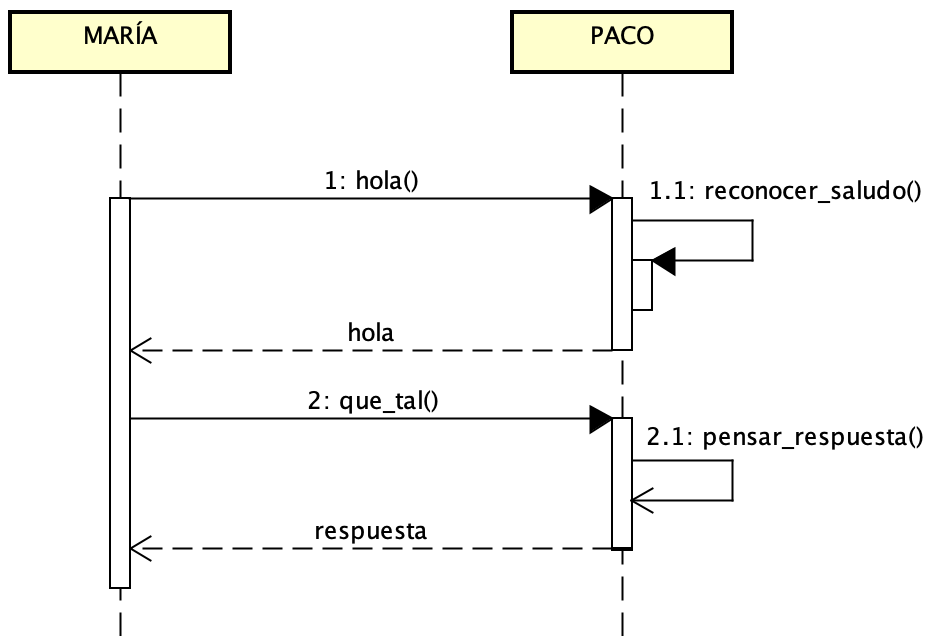
\includegraphics[width=10cm]{./img/sequence/human.png}
    \caption{Secuencia de Comunicación humana}
    \label{fig:humanseq}
\end{figure}

Como se puede ver en la figura \ref{fig:humanseq}, un protocolo de comunicación entre dos personas se basaría en un saludo para entablar conversación, para posteriormente realizar una pregunta.

En el caso de los asistentes, el proceso de conversación se basa en lo mismo: un usuario saluda al asistente mediante el uso de una palabra o conjunto de palabras, al que se llamará \textbf{hotword}, que cuando sea reconocido por el asistente inteligente, devolverá el saludo.
Es entonces cuando el usuario debe realizar la pregunta o solicitar la información que requiera.
Una vez hecha la pregunta, el dispositivo se pondrá a pensar la posible respuesta, entrando en el proceso al que se llamará \textbf{reconocimiento de los hechos}. Una vez identificados los hechos, devolverá la respuesta que más se acerque a lo deseado, gracias a un entrenamiento previo.

\newpage
\subsubsection{Cómo Piensa el Asistente}

El proceso de pensamiento analizado de los principales asistentes del mercado, que se expondrá en el presente capítulo, tiene una estructura similar independientemente del tipo de asistente que se trate, asemejándose a la figura \ref{fig:humasseq}.

\begin{figure}[h!]
    \centering
    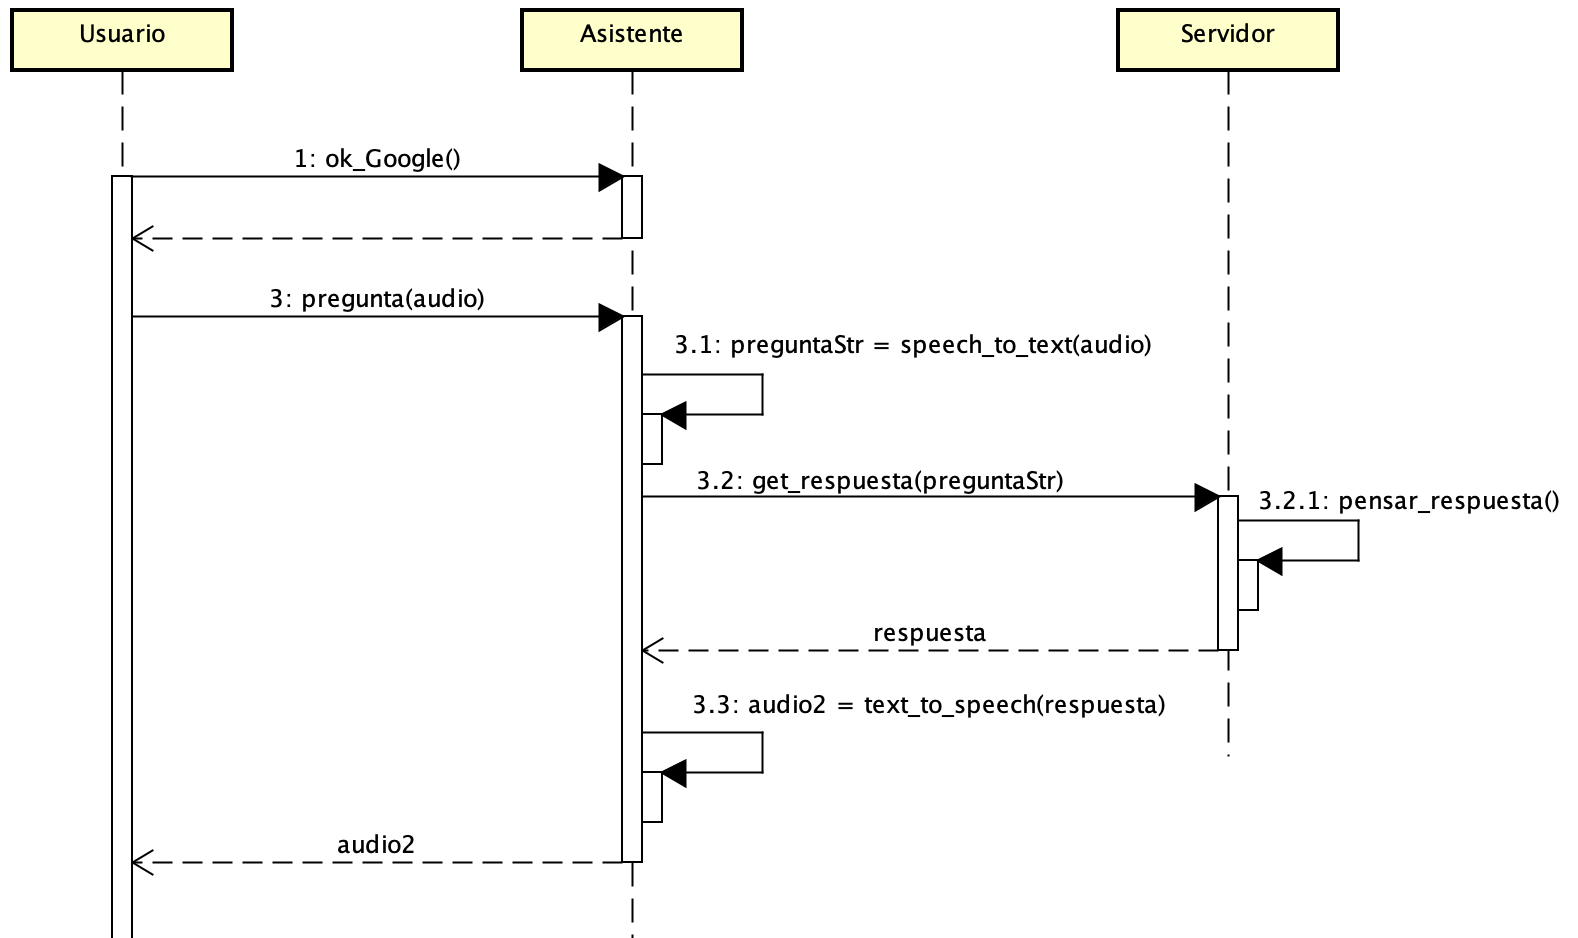
\includegraphics[width=13cm]{./img/sequence/humasseq.png}
    \caption{Secuencia de Comunicación humano-asistente}
    \label{fig:humasseq}
\end{figure}

Lo que diferencia a un asistente de otro, es la manera en la cual piensa la respuesta, dando mayor validez a un asistente que dé una respuesta más aproximada a lo solicitado.
Para lograr dar la respuesta más acertada, la mayoría de los asistentes existentes realizan el procesamiento de la respuesta en la nube debido a la gran cantidad de información que tienen previamente almacenada de otras consulta de otros usuarios para contrastar los hechos capturados, al igual que también pueden realizar en la nube el proceso de speech-to-text enviando los audios a sus servidores y transformándolo ahí a cadenas de texto, o el de text-to-speech, que sería el proceso inverso.


\section{Requisitos mínimos}
Una vez que ya se ha expuesto cual es el funcionamiento base de un asistente virtual inteligente, interesa saber cuál es de todos los existentes que más se adecúa a las necesidades establecidas para este proyecto, de manera que se le exijirá que cumpla el máximo de los siguientes puntos expuestos.

\subsubsection{Despliegue en Dispositivos}

El asistente seleccionado debe poder ser desplegado de manera gratuíta en un dispositivo formado por una placa RasbperryPi, o similar.

Para ello, se requiere que el asistente disponga de una librería o de un modo de uso que se pueda implementar en un dispositivo pequeño y portátil, facilitando el cambio de una ubicación física por otra de los distintos posibles puntos que existen dentro de un hogar, manteniendo una instalación lo más simple y limpia posible, en la que solo sea requerida la localización de un enchufe activo que posea corriente eléctrica.

\subsubsection{Tratamiento de la Información}

El asistente debe seguir la Ley Orgánica de Protección de Datos~\cite{lopd}, y no debe tener acceso a escuchar conversaciones ajenas violando la intimidad de los usuarios.

Cualquier vacío legal o conjunto de cláusulas de extensa longitud no podrá será aceptado, para poder asegurar la protección de los datos de los usuarios.

En caso de almacenar algún tipo de dato, debe poder ser público para el usuario en cuestión, o haber sido aceptado expresamente por el usuario a favor de un control de su seguridad.

\subsubsection{Conexión a Internet}

La orientación de un dispositivo asistente inteligente como este a personas de una edad avanzada debe tener en cuenta que es posible que la mayoría de sus usuarios potenciales no tengan una conexión a internet en sus respectivos hogares.

Esto provoca que la conexión del dispositivo a la red tiene que ser lo mínima posible, favoreciendo los asistentes en los cuales el proceso de pensamiento sea ejecutado dentro del propio dispositivo, evitando tener que hacer el cálculo e identificación en servidores de alojados en la nube.

Es decir, el dispositivo debe ser capaz de funcionar en el lugar más remoto posible y sin ninguna conexión a internet, simplemente tras ser conectado a una red eléctrica.

\subsubsection{Adicción de Nuevas Tareas}

El software del asistente inteligente debe tener la capacidad de añadir nuevas tareas fácilmente, de modo que se puedan añadir nuevas funciones tanto propias, como desarrolladas por la comunidad de Internet.

\section{Mercado}
\label{mercato}
En los siguientes apartados se mostrarán las diferentes opciones que ofrece ya el mercado para el uso de asistentes inteligentes, con el fin de comprobar la existencia de alguno que ya tenga establecidos los requisitos base ya descritos, o que permita la opción de poder establecerlos.

    \subsection{Google Assistant}
    El asistente inteligente de Google es el que está en el año 2020 a la cabeza de los asistentes virtuales~\cite{top-asistentes}, y esto es debido a que viene instalado en todos los dispositivos Android, ocupando estos dispositivos la mayor parte del mercado de la telefonía móvil. Esta posición privilegiada le proporciona un mayor entrenamiento, dando por resultado una elevada tasa de acierto que como consecuencia le atribuye mayor usabilidad.

Esta creación de Google tiene una gran aceptación con los diferentes aparatos existentes para la domótica del hogar, facilitando la implementación y realización de tareas:

- Una tarea es un conjunto de acciones que se llevan a cabo tras accionarse un evento que hace de interruptor, pudiendo ser el evento tanto un comando de voz, la pulsación de un interruptor o la activación de un sensor, entre otras opciones.

De esta manera, Google permite el control de la domótica del hogar, o la realización de diferentes acciones en nuestro día a día, pero requiere ser configurado por cada usuario, evitando por tanto la posibilidad de un despliegue común.

\subsubsection{Cómo Funciona}

El proceso de pensamiento que hace el asistente de Google está basado en la nube, pero no solo eso sino que Google hace en sus servidores también el proceso de Speech-to-Text.

De este modo, Google almacena todos los audios\cite{google-almacena} que se le mandan a través de su asistente, estudiándolos uno a uno y asegurando o corrigiendo sobre la respuesta que envió el asistente.

Este proceso de corregir o confirmar es el método que tiene Google de entrenamiento, de manera que en la próxima consulta sobre el mismo tema, el asistente pueda responder con mayor exactitud.

Queda claro que sobre la teoría es un buen plan de entrenamiento, y en un mundo ideal esto sería perfecto, pero esos audios también pueden contener parte de información privada, o pueden servir para espiar conversaciones privadas que un usuario puede no querer que estén almacenadas, ni que sean escuchadas por otra persona, aunque sea un propio trabajador.

En cuanto a la posibilidad de ser desplegado en otro dispositivo que no sea un smartphone o una tablet, Google nos lo pone fácil, ya que otorga una librería con la cuál facilita la instalación y uso en una gran variedad de dispositivos, cuyo requisito es que dispongan de conexión a Internet.


    
    \subsection{Amazon Echo}
    ~También conocido como Alexa, es la opción creada por Amazon que más fuerza está tomando en la sociedad para ser elegida como el asistente de voz inteligente que nos acompañe en nuestro día a día.

A pesar de todas las ventajas posibles similares a las que se han descrito para el asistente de Google, también comparte sus contras, como las referentes a la localización donde se procesan los audios y donde se efectúa el entrenamiento, por lo que es otra opción que va a ser rechazada.

Sin tener en cuenta la ubicación del proceso de pensamiento, Amazon asegura\cite{escandalo-amazon} que almacena todos los audios hasta que es el propio usuario quien decide borrarlos, pero aún con la solicitud expresa del usuario no pueden ser borrados completamente ya que han sido compartidos con terceros, que son quienes han desarrollado funciones específicas, llamadas Skills. Estos desarrolladores no solo tienen acceso a los audios sino que los poseen, pudiendo hacer una mala práctica con ellos.

Por tanto, aunque el usuario en cuestión pida a Amazon el borrado de estos ficheros, la compañía únicamente podría borrar los archivos que posee, permaneciendo todos los cuales un desarrollador de estas skills haya almacenado, sin permitir que el propio Amazon sea capaz de eliminarlos aunque tratase de hacerlo.
    
    \subsection{Mycroft}\label{Microft}
    Ante la falta de privacidad por parte de Google y Amazon, se abre la puerta a Mycroft, proyecto Open Source que busca como pilar la seguridad de los datos y la protección de la privacidad, de manera que asegura no almacenar ningún dato o información del usuario potencial.~\cite{mycroft-doc}

Mycroft tiene una de las mayores comunidades OpenSource activa para el desarrollo e implementación de asistentes~\cite{mycroft-com}, de modo que dispone de una gran cantidad de skills que añadir a nuestro dispositivo, posicionándose como opción principal para la elaboración del proyecto.

Este asistente virtual puede ser fácilmente implementado en dispositivos tales como Raspberry, cumpliendo los propósitos y requisitos de este proyecto.

En cuanto a la conexión a Internet, el equipo de Mycroft informa acerca de estar trabajando en una herramienta que permita desplegar el asistente ya entrenado dentro del dispositivo, evitando la conexión, pero de momento esa herramienta no está finalizada, por lo que cojea en ese aspecto y de momento, debería tener una conexión permanente.

En caso de que estén en lo cierto y estén trabajando en esa herramienta, este asistente ocuparía la primera opción como asistente a desplegar, pero en el momento actual en el cual este proyecto cobra vida, no es viable su implementación.


    
    \subsection{Snips AI}
    Snips Seeed es una  plataforma de inteligencia artificial para el desarrollo de dispositivos asistentes.

Esta plataforma nos permite crear nuestro propio asistente basándose en un entrenamiento previo con unos hechos predefinidos por el desarrollador.

En ese entrenamiento previo, se permite al asistente tomar lo aprendido de otros skills, que son fáciles de añadir.

Tras la implementación en el dispositivo físico, el asistente ya ha sido entrenado, por lo cual no necesitaría volver a estar conectado a internet, siendo este el mayor argumento a favor ya que es la carencia del resto de asistentes.

En cuanto a su uso, el dispositivo solamente se mantiene a la espera de poder recibir el \textit{hotword}. Este hotword puede ser modificado por cualquier otra palabra que se desee, lo cual beneficia al proyecto actual con la posibilidad de asignar una palabra más acorde y familiar a las personas a quienes va orientado.

El asistente, en cuanto a su configuración interna, sigue el protocolo de comunicación descrito en la figura \ref{fig:humasseq}, con una pequeña modificación:
Cuando el servidor ya ha entendido la pregunta o solicitud, genera unos hechos definidos en su entrenamiento en forma de objeto que envía a través de un puerto MQTT, y se queda a la espera de una respuesta.

Los otros skills, que han sido añadidos previamente en el entrenamiento, están levantados escuchando por el puerto, de manera que identifican los objetos que circulan por él y comprueban si ese hecho le corresponde, que de no ser así, simplemente lo ignoran.
Una vez que un skill captura un hecho que sí que le corresponde, comprueba los \textit{slots} que contiene dicho hecho para ver qué es lo que se está solicitando. Tras esto, genera una respuesta en forma de cadena de texto, y la envía por el puerto MQTT para que la recoja el \textit{skill-server}.

Una vez capturada por este, simplemente transcribe el mensaje a audio con su skill de text-to-speech, y se lo transmite al usuario a través del altavoz, finalizando la comunicación.

Como se puede ver, el tratamiento de la información que se le otorga al dispositivo es el que nosotros deseemos, ya que el asistente no envía nada al exterior. De esta manera, nosotros controlamos qué sucede con la información, siendo el otro punto requerido en la búsqueda de un asistente ideal.

Como extra, Snips Seeed es una plataforma gratuita que se basa en una colaboración de una gran comunidad de desarrolladores. Pese a ser esta comunidad de menor tamaño que la conseguida por la opción de Mycroft, hay una gran cantidad de aplicaciones disponibles como juegos, la consulta del tiempo o la consulta de noticias, preparadas para ser asignadas directamente a nuestro dispositivo.

Como se puede ver, SnipsSeeed otorga las herramientas necesarias para cumplir todos los requisitos estipulados anteriormente, siendo la plataforma que se pone a la cabeza como posible elección.

    
    \subsection{Elección Final}

La elección más acorde de entre todas las propuestas es el uso Snips AI, ya que se adapta a todos nuestros requisitos.

En cuanto al proyecto, va a ser necesario el desarrollo de un dispositivo que contenga este asistente, al igual que el diseño y desarrollo de un backend capaz de albergar la información relativa a cada dispositivo.

Para la gestión de estos dispositivos también será necesaria la implementación de una página web, desde la cual puedan ser los dispositivos configurados, manejados y controlados.

La implementación operativa de todo este sistema formaría un proyecto de gran envergadura, por lo que en los siguientes capítulos se documentará el diseño y desarrollo del backend y del frontend, mostrando el control y gestión real de un dispositivo el cual su rango de funciones será breve, de modo que se establezca la base y se explique como puedan ser añadidas nuevas funciones de una manera simple y sencilla.


\chapter{Plan de Desarrollo}\label{cap.desarrollo}
\section{Introducción}
En el siguiente capítulo se mostrará cual ha sido el método por el cual se ha desarrollado el proyecto, al igual que se definirán las fases del plan de desarrollo a seguir.

También se mostrará y explicará cuales han sido tanto las herramientas utilizas, como las librerías necesarias para una correcta implementación y desarrollo del proyecto con el fin de acercar al lector a entender cómo se ha diseñado, y qué es lo necesario para poder replicar el contenido del mismo en otros proyectos similares.



\section{Metodología}
Para el desarrollo de este proyecto se ha escogido una implementación siguiendo la combinación de un modelo iterativo y un modelo incremental.~\cite{mod-it-inc}

Este método puede describirse de una manera simple y rápida, basada en la repeticion de ciclos en los cuales se van mejorando las funcionalidades implementadas a partir de la experiencia del usuario, y añadiendo nuevas.

Cada ciclo puede describirse como la continuación de los siguientes pasos:

\begin{enumerate}
    \item El desarrollador muestra un prototipo.
    \item El usuario lo prueba.
    \item El usuario muestra su experiencia tanto positiva como negativa, comentando posibles mejoras y proponiendo nuevas funcionalidades.
    \item Se subsanan esas carencias.
    \item Se obtiene una nueva versión del prototipo.
    \item Vuelta al paso inicial.
\end{enumerate}{}

La elección de este modelo se debe, por tanto, a la naturaleza del proyecto del cual se trata: al estar trabajando con unas nuevas tecnologías, y no tener muy claras las capacidades de las cuales los posibles asistentes están dotados, es preferible realizar un desarrollo basado en la entrega de pequeños prototipos que nos vayan ampliando el conocimiento de todas las posibilidades que van a poder ser implementadas, al igual que produce una retroalimentación a partir de la experiencia del usuario, siendo bastante útil tanto para mejorar, como para eliminar o para añadir nuevas funcionalidades.

En el caso del presente proyecto, el usuario el cual realiza las pruebas del prototipo se trata del propio tutor del proyecto, el cual otorga su experiencia, experiencia que está curtida a través de años de trabajo y perfeccionamiento, siendo más sabia que la del propio desarrollador, ayudando a elaborar un rediseño de las características que aumente la usabilidad. 

\section{Planificacion}
\label{planificacion}

Una vez conocido el método de trabajo que se seguirá para el desarrollo del proyecto, se deben conocer los plazos en los cuales el proyecto debe ser finalizado y entregado.

La fecha de inicio del proyecto es, por tanto, \textit{el 15 de Octubre de 2019}, y la fecha límite en la cual el proyecto debe ser entregado data del \textit{29 de Febrero de 2020}.

\subsubsection{Disponibilidad del desarrollador}

El proyecto se debe ajustar a una extensión de 300 horas, como fué especificado en el cálculo de costes en el apartado \ref{duracion_proyecto} del presente documento.

En cuanto a la disponibilidad del proyecto, el desarrollador carece de suficiente tiempo  al día como para elaborar 8 horas díarias, asemejándose a un trabajo real, debido a tener que compaginar las 7 horas diarias de un trabajo externo, con las necesarias para la completitud de dos asignaturas de la Universidad, y el presente proyecto.

Tras una planificación semanal, el desarrollador es capaz de asignar una media de 24 horas semanales, lo que supondría poder finalizar el proyecto en:

\begin{center}
    \textit{24horas/semana / 6 dias laborables/semana = 4horas/dia }
    
    \textit{300horas / 4 horas/dia = 75 días }  

\end{center}

\newpage
\section{Diagramas de Gantt}

Al datarse de un proyecto basado en prototipos y dada la amplitud posible del mismo, se va a proceder a organizar el plan de trabajo en la secuencia del siguiente ciclo:
\begin{enumerate}
    \item \textit{Elicitación de requisitos} \newline
    Periodo en el cual se razona cuáles son los requisitos necesarios que se van a llevar a cabo en el protototipo a desarrollar. En es este periodo en el cual se realiza el diagrama de Gantt del prototipo indicado, planeando y estipulando los tiempos necesarios para llevar a cabo cada tarea.
    
    \item \textit{Desarrollo} \newline
    Esta etapa es en la cual se lleva a cabo la elaboración del prototipo siguiendo el plan de desarrollo estipulado en el punto anterior.
    
    \item \textit{Presentación del prototipo} \newline
    Reunión con el tutor para mostrar el prototipo y sus funcionalidades, con el fin de ver si se ha alcanzado lo esperado, al igual que para realizar un brainstorm conjunto con el fin de poder elicitar los requisitos del prototipo siguiente.
\end{enumerate}

La cuantía de prototipos elaborados será tanta como permitan las 300 horas de duración máxima del proyecto, enfocando cada prototipo en la completitud de un mínimo de requisitos con los cuales se busca un acercamiento a un prototipo final lo más aproximado posible a un producto final.

Debido a la condición del desarrollador que va a llevar a cabo el proyecto, se considera que cada día marcado en los siguientes diagramas corresponde con 4 horas de trabajo.

Para llevar a cabo la organización, se ha respetado un día libre a la semana, el cual coincide con el Domingo, al igual que se respetan los días festivos nacionales.

\textit{NOTA: Finalmente, tras la elaboración iterativa y ajuste de prototipos a las horas máximas marcadas se ha conseguido elaborar la cuantía de 4 prototipos, de los cuales se mostrarán sus diagramas de Gantt a continuación.}

\begin{sidewaysfigure}
\begin{figure}[H]
    \centering
    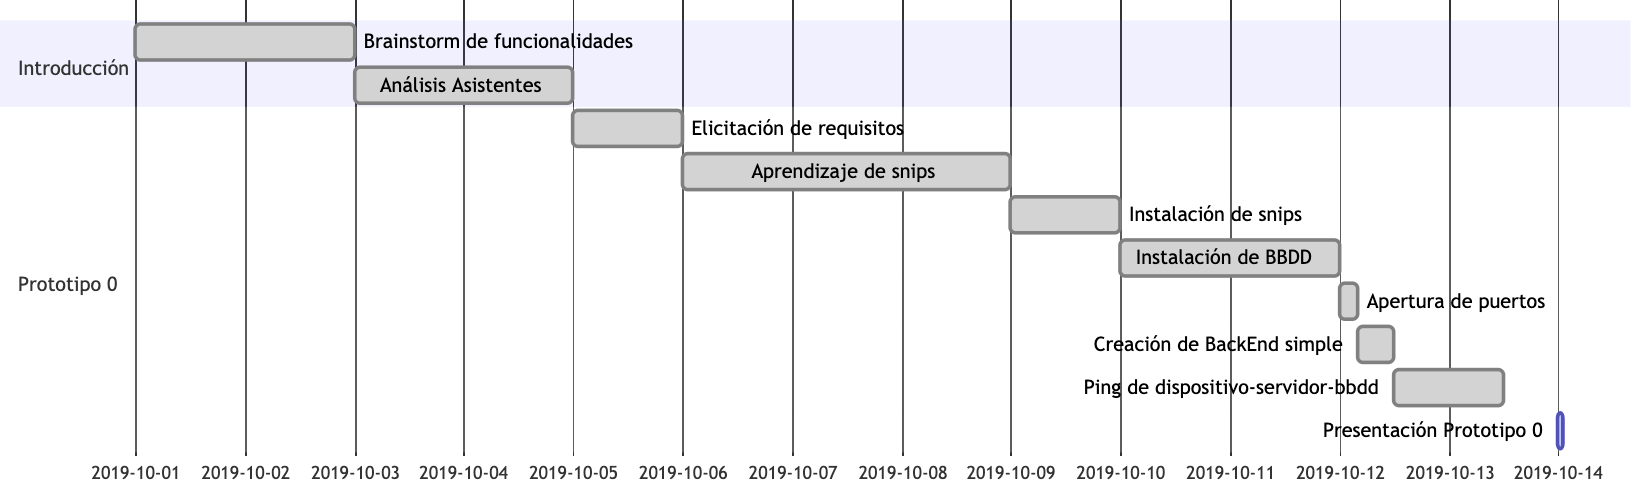
\includegraphics[width=19cm]{./img/grantt/p0.png}
    \caption{Diagrama de Gantt - Prototipo 0}
    \label{fig:grant.p0}
\end{figure}
\end{sidewaysfigure}

\begin{sidewaysfigure}
\begin{figure}[H]
    \centering
    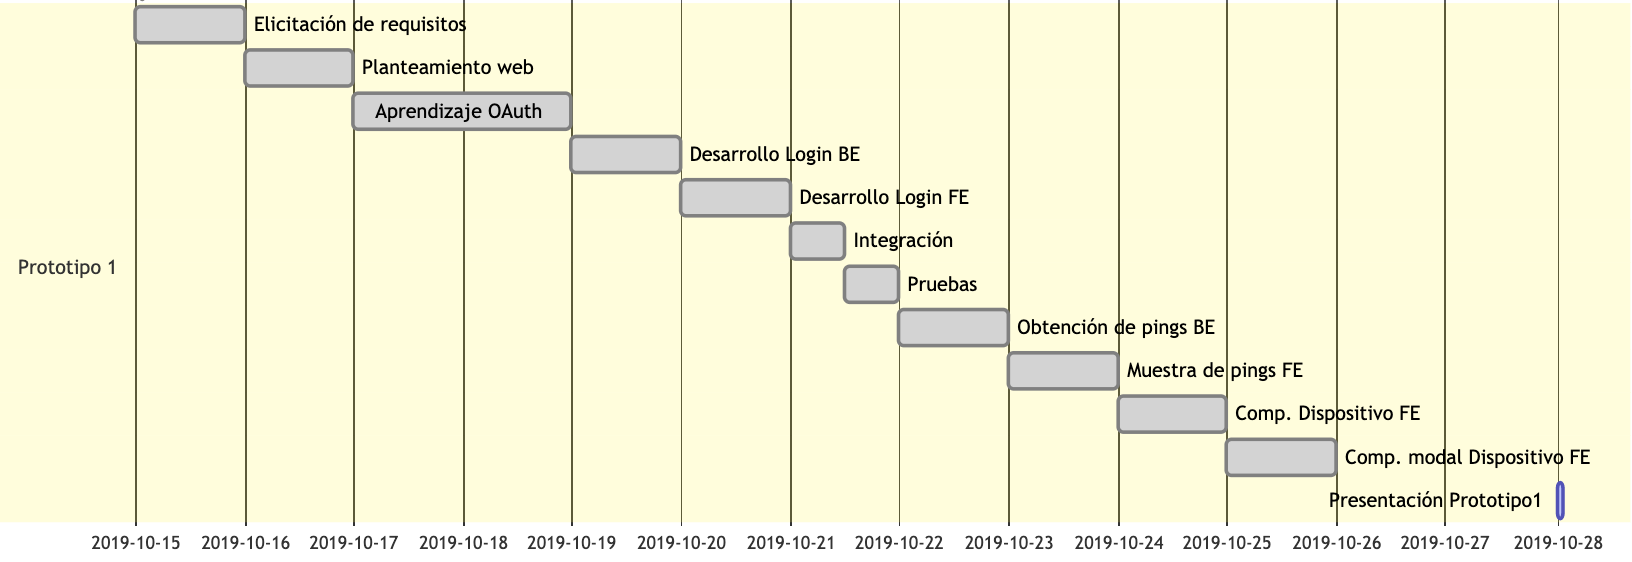
\includegraphics[width=19cm]{./img/grantt/p1.png}
    \caption{Diagrama de Gantt - Prototipo 1}
    \label{fig:grant.p1}
\end{figure}
\end{sidewaysfigure}

\begin{sidewaysfigure}
\begin{figure}[H]
    \centering
    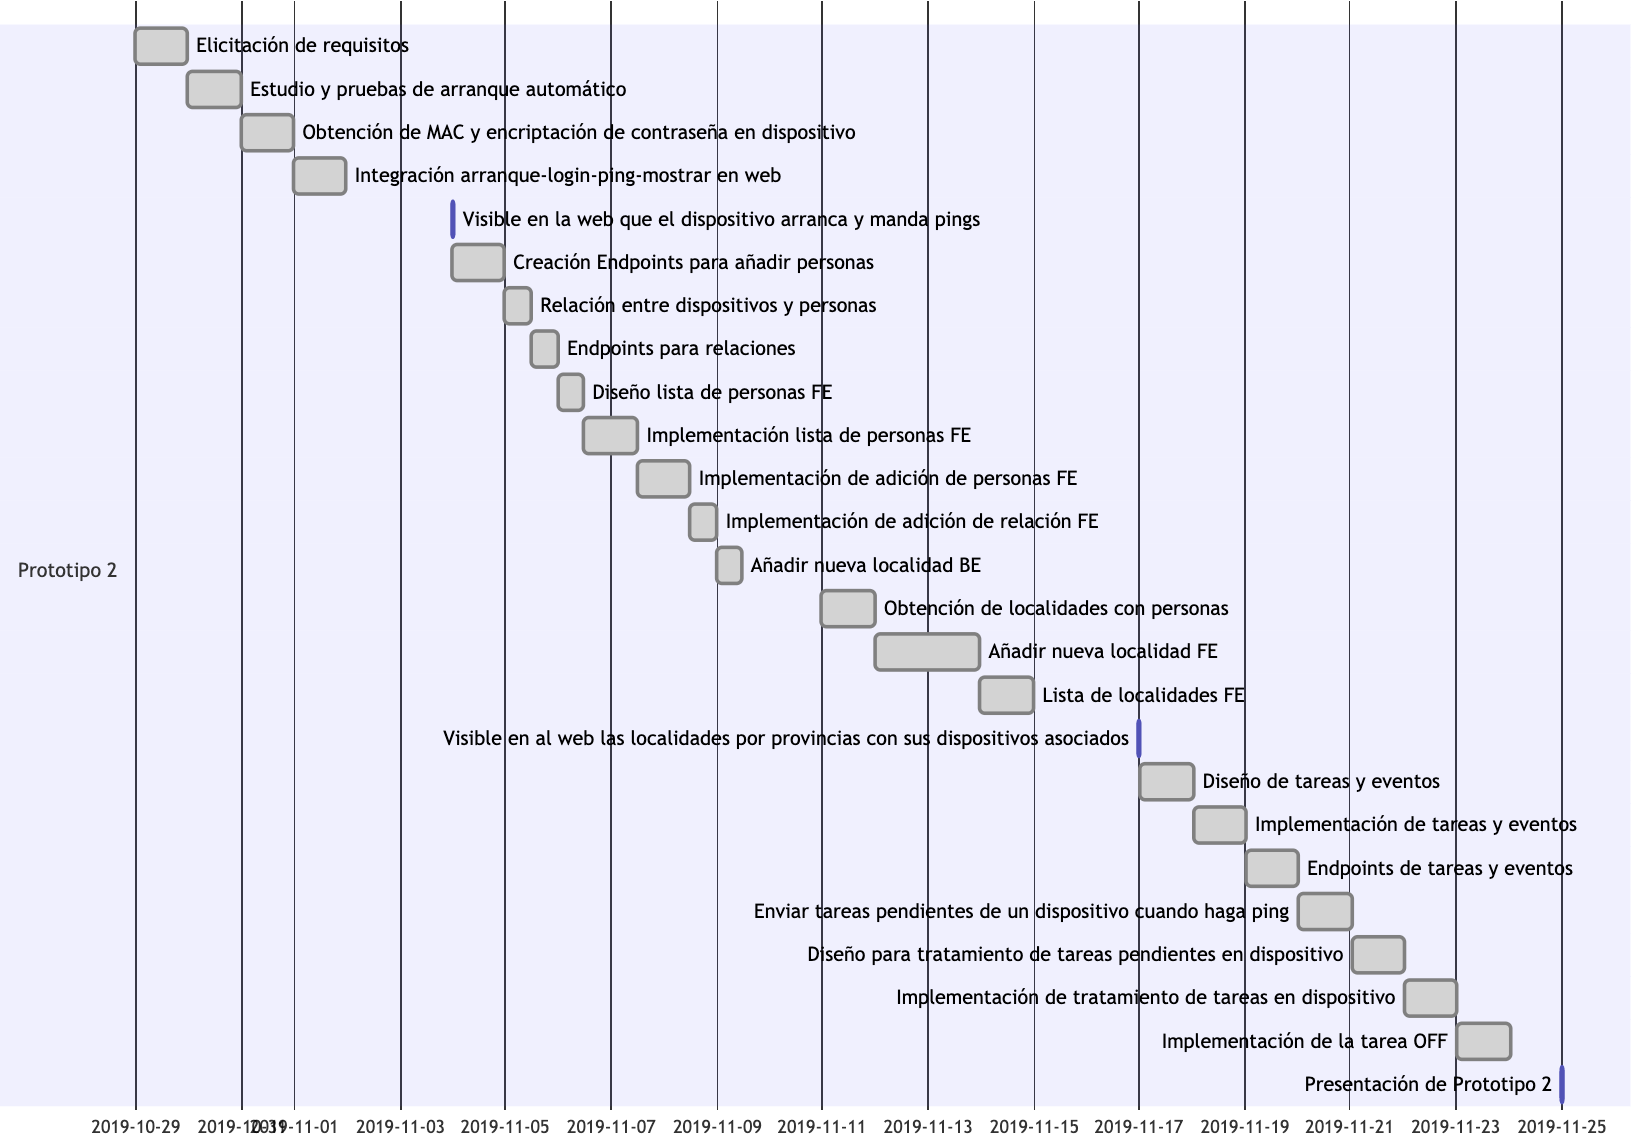
\includegraphics[width=19cm]{./img/grantt/p2.png}
    \caption{Diagrama de Gantt - Prototipo 2}
    \label{fig:grant.p2}
\end{figure}
\end{sidewaysfigure}

\begin{sidewaysfigure}
\begin{figure}[H]
    \centering
    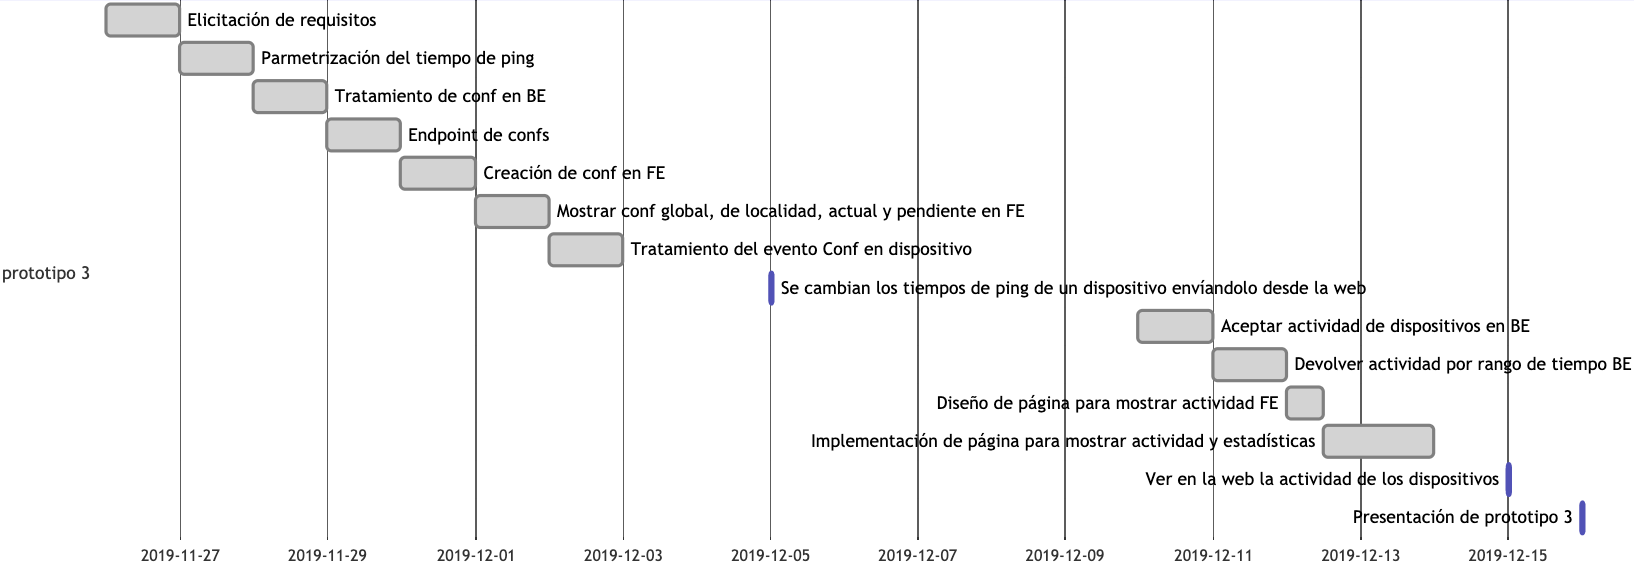
\includegraphics[width=19cm]{./img/grantt/p3.png}
    \caption{Diagrama de Gantt - Prototipo 3}
    \label{fig:grant.p3}
\end{figure}
\end{sidewaysfigure}

\begin{sidewaysfigure}
\begin{figure}[H]
    \centering
    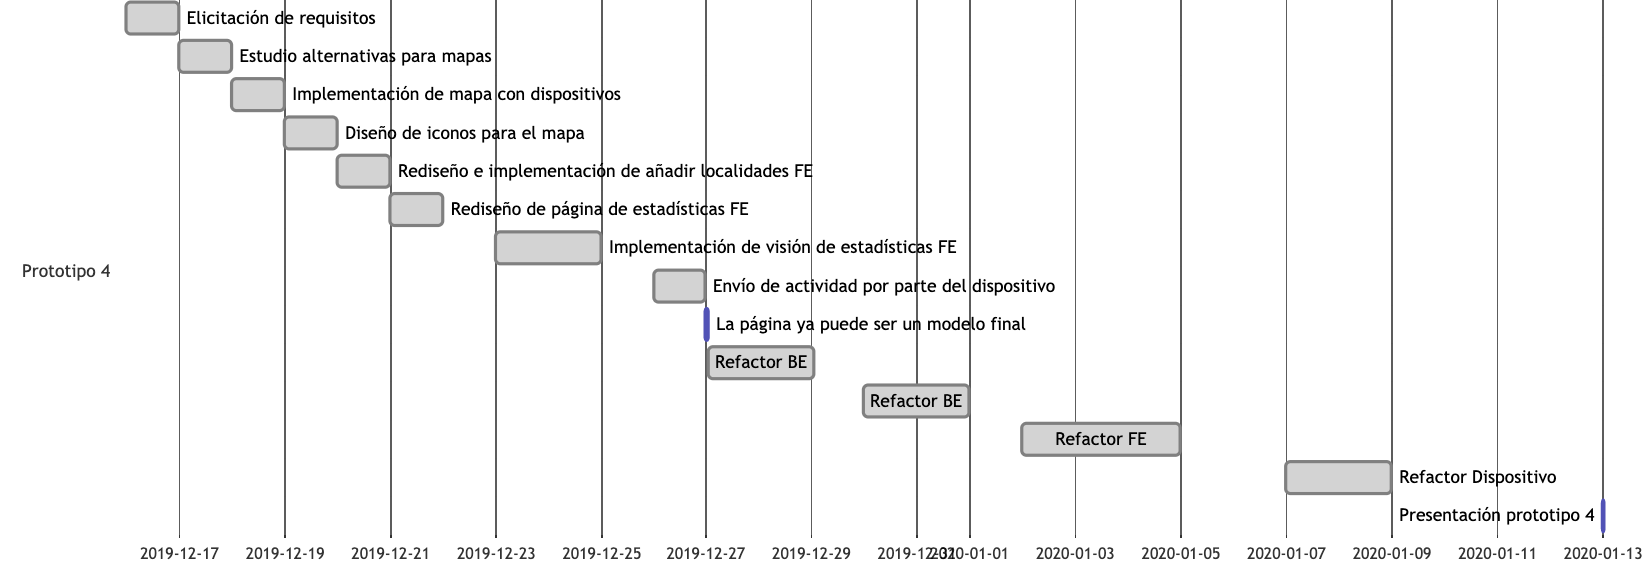
\includegraphics[width=19cm]{./img/grantt/p4.png}
    \caption{Diagrama de Gantt: Prototipo 4}
    \label{fig:grant.p3s}
\end{figure}
\end{sidewaysfigure}

\newpage
\section{Recursos y herramientas}
Para una correcta implementación que se adecúe a los requisitos, al igual que para un futuro mantenimiento del proyecto, enumerarán a continuación las herramientas que han sido utilizadas durante su desarrollo, con el fin de poder replicar en un futuro el entorno de trabajo en un futuro, o poder entender mejor cómo ha sido implementado.

    \subsection{Kotlin}

Kotlin es un lenguaje de programación funcional desarrollado por el equipo ruso de JetBrains como una evolución a Java por excelencia, permitiendo una interoperabilidad entre ambos, utilizándose bajo la JVM.

La sintaxis de Kotlin lo hace más intuitivo y simple, llegando al mismo resultado que en Java pero en un menor número de líneas, ahorrando tiempo y espacio.

Pese a que su gran popularidad es por el desarrollo Android, ahora está creciendo en su utilización en el lado del servidor gracias al framework de Ktor.~\cite{ktor}

    \subsection{Ktor}

Es un framework que se aprovecha de la usabilidad de Kotlin para el desarrollo de clientes y servidores asíncronos en la implementación de sistemas conectados.

Este framework será añadido al proyecto a través de la instalación de sus dependencias en gradle a través del fichero \textit{./build.gradle}.

    \subsection{Koin DI}
    \label{Koin}

Koin es un inyector de dependencias compatible con Kotlin, siendo bastante útil para poder aplicar el principio de inversión de dependencias en el desarrollo del backend.~\cite{koin}

La configuración de este inyector de dependencias es bastante simple, teniendo una sintaxis sencilla y útil en la que únicamente hay que utilizar Kotlin, evitando así los ficheros de configuración en XML que obligan a usar otros tipos de inyectores.

La utilización de este framework será útil para poder aislar los casos de uso del sistema, de modo que no tengan dependencia de ninguna otra clase u servicio externo a los casos de uso, aumentando la escalabilidad del sistema y permitiendo una extensibilidad de los casos de uso en un futuro.

Para su utilización, se añaden las dependencias al fichero \textit{./build.gradle}.

Se implementará a través de la instalación de su módulo en el main de la aplicación.
\begin{lstlisting}
    // Declare Koin
    install(Koin) {
        modules(myModule)
    }
\end{lstlisting}

y en el módulo de Koin se indicarán los servicios que serán inyectados.
\begin{lstlisting}
// app.di.Module.kt

/**
 * This module has got the Koin configuration with the declarations of the needed instances.
 * This instances could be injected now, applying the dependency inversion principle.
 */
val myModule = module {
    single { ConfRepo() as ConfService }
    single { DeviceRepo() as DeviceService }
    single { LocationRepo() as LocationService }
    single { PeopleRepo() as PeopleService }
    single { TaskRepo() as TaskService }
    single { UserRepo() as UserService }
    single { IntentRepo() as IntentsService }
    single { TokenCtrl() as AuthService }
}
\end{lstlisting}


    \subsection{OAuth 2.0}
    \label{oauth20}
    
OAuth 2.0 es un protocolo que establece las pautas para una conexión segura entre un servidor y un cliente.
Este protocolo se basa en la implementación de un servidor de tokens frente al cual hay que estar identificado.~\cite{oauth2}

La secuencia correcta para la utilización de este protocolo consta de los siguientes pasos:

\begin{enumerate}
        \item El usuario manda sus credenciales al sistema.
        \item El sistema comprueba que sus credenciales son correctas.
        \item El sistema solicita al servidor OAuth un nuevo inicio de sesión para un cierto usuario con las ciertas características.
        \item El servidor OAuth provee al sistema un conjunto de token temporales: uno de acceso que utilizará el usuario para identificarse, y otro de refresco para que recupere el de acceso en caso de que se le caduque.
        \item El sistema devuelve los tokens al usuario
\end{enumerate}
Una vez que el usuario ya dispone de los tokens, simplemente tiene que realizar las peticiones normales a los end-points~\cite{endpoint} del sistema pero introduciendo el token de acceso en la cabecera de autorización en cada llamada, de modo que el sistema lo toma, comprueba contra el servidor OAuth2.0 que sigue siendo un token válido, y en caso de serlo, deja realizar al usuario la petición.

Para la implementación de este protocolo utilizaremos un framework adaptado a la lógica de Ktor.~\cite{myndocs.oauth2}

Este framework será adaptado a las características de uso del sistema, estableciendo el método de comprobación de credenciales que se considere oportuno, pudiendo variar en caso de que las credenciales correspondan con las de un dispositivo, o con las de un administrador del sistema.

\begin{enumerate}
    \item Añadir sus dependencia al fichero \textit{./build.gradle}.
    \item La adaptación de sus clases de identificadores y tienda de tokens con el fin de poder hacer una comprobación de credenciales y autenticar los tokens como requiera el sistema. Para ello, se han modificado dos clases: \textbf{InMemoryTokenStoreCustom} y \textit{InMemoryIdentityCustom}, las cuales se albergan en \textit{./app/oauth}.
    \item Instalación del servidor OAuth2.0 en nuestra aplicación.
    Dentro de \textit{./app/Application.kt}, instalamos el servidor:

    \begin{lstlisting}
        // instance of tokenStore manage tokens
        tokenStore = InMemoryTokenStoreCustom.get()
        
        // Install and configure the OAuth2 server
        install(Oauth2ServerFeature) {
            // set the custom store to have access -> Singleton Pattern
            tokenStore = InMemoryTokenStoreCustom.get()
        }
    \end{lstlisting}
\end{enumerate}

    \subsection{Exposed SQL}

Exposed SQL es un framework que simplifica el acceso a la base de datos evitando las consultas puras de SQL mediante una sintaxis más simple que tiene definida en su \textbr{DSL}.~\cite{exposedsql}

El método por el cual se ha accedido al uso de este framework es por su facilidad para parsear los resultados obtenidos en cada consulta, al igual que para limitar los posibles ataques por \textbr{inyección de SQL}.

    \subsection{JSoup}

JSoup es una librería que permite la obtención del código fuente HTML resultante de sitios web, dando las herramientas necesarias para la captura y parseo de los diferentes valores en función de las etiquetas, clases, y jerarquía de los distintos elementos HTML obtenidos.~\cite{jsoup}
    
    \subsection{PostgreSQL}
    \label{postgresql}
También conocido como postgres, es un sistema de gestión de bases de datos relacionales, por lo que permite una orientación a objetos en las relaciones de los elementos contenidos en sus diferentes tablas.
Postgres es libre y de código abierto, lo que nos permite su uso en el proyecto.

    \subsection{VueJS}
    \label{Vue}

VueJS es un framework JavaScript que permite la creación y desarrollo de diferentes aplicaciones web.
Entre sus ventajas está su reactividad, permitiendo cambiar la información mostrada en la web de manera dinámica, evitando tener que recargar la página. 

Otro aspecto por el cual elegir este framework está en su simplicidad para crear e importar componentes, al igual que para enviar la información entre ellos.

También cabe destacar su modularidad: VueJS parte de cero, de modo que toda función de la que queramos disponer, simplemente tendrá que ser importada, pudiendo adaptar cualquier librería JavaScript fácilmente. Esto permite un mayor acceso a todas las librerías ya existentes, al igual que la creación de un proyecto con un menor peso final, al contener únicamente las librerías que son necesarias.

El aspecto más importante por el cual VueJS está siendo utilizado es su curva de aprendizaje, característica con la que todo el mundo concuerda: es más fácil de aprender a utilizar que sus principales competidores, entre los cuales se encuentran Angular y React.~\cite{vue-curve}

    \subsection{Bootstrap-Vue}

Bootstrap-Vue es una adaptación de la librería de componentes Bootstrap que permite la utilización de sus componentes en VueJS de una manera más simple y rápida.~\cite{bootstrap-vue}

    \subsection{Leaflet}

Leaflet es una biblioteca JavaScript basada en OpenMaps, permitiendo la utilización e implementación de mapas en nuestras páginas web de una manera gratuita gracias a ser de código abierto.~\cite{leaflet}

Leaflet tiene un gran desarrollo por parte de la comunidad, lo que hace a esta librería más interesante para la implementación de diferentes funciones, como puede ser la adición de cualquier tipo de marca en el mapa, la geocodificación a través de los atributos de un punto exacto como puede ser su calle o código postal, y permitiendo también la geocodificación inversa, obteniendo esos datos de un punto exacto a partir de las coordenadas.

    \subsection{Material icons}

Es la librería de iconos gratuita de Google, la cual sigue los estilos de diseño de Material Design, basada en un estilo limpio y simple.

    \subsection{Astah UML}
Es una herramienta cuya función es la creación de diagramas y esquemas UML, que nos será muy útil para realizar el diseño y organizar el desarrollo del sistema.



\chapter{Análisis del Proyecto}\label{cap.analisis}
\section{Introducción}
Una vez elegido el tipo de asistente virtual inteligente en el capítulo previo, en el presente capítulo se procede al análisis tanto de requisitos que debe cumplir el sistema, como de las funcionalidades que debe tener la página de administración, pasando por las operaciones que debe de ser capaz de realizar el dispositivo.

\section{Requisitos}

Para poder identificar qué es lo que se debe implementar, se debe realizar primero una identificación de las necesidades técnicas del proyecto a desarrollar, con el fin de identificar cuales son las implementaciones que se deben desarrollar.

\subsection{Requisitos Funcionales}

Los requisitos funcionales son un conjunto de funciones que debe poder servir el proyecto. Están basados en especificar qué es lo que el sistema debe ser capaz de hacer o permitir, y son los siguientes:

    \label{req.fun}
\begin{enumerate}[label=RF\arabic* -]
    \item Los dispositivos deben ser capaces de identificarse ante el sistema.

    \item El sistema debe permitir obtener un nuevo token de acceso mediante un token de refresco.

    \item El sistema debe ser capaz de registrar nuevos dispositivos.

    \item El sistema debe devolver un par de tokens de autenticación a los dispositivos que se identifiquen.

    \item El dispositivo debe informar al sistema sobre su estado cada un cierto tiempo, que pueda ser configurable, siendo guardado en un fichero de configuración.

    \item El sistema debe poder actualizar remotamente el archivo de configuración tanto de dispositivos particulares, como de dispositivos de una misma localidad, como de todos los dispositivos en conjunto.

    \item El sistema debe poder asignar tareas a un dispositivo, a una localidad, o a todos los dispositivos.

    \item El sistema debe ser capaz de mandar tareas pendientes a realizar a un dispositivo, como puede ser actualizar su archivo de configuración, apagar el dispositivo, o reiniciarlo, cuando el dispositivo informe de que esté conectado.

    \item El dispositivo debe realizar las tareas por fecha de creación.

    \item El dispositivo debe informar al sistema cada vez que proceda a realizar una tarea.

    \item El sistema debe poder marcar tareas de un dispositivo específico como ya realizadas, guardando la fecha de realización.

    \item El sistema debe ser capaz de recibir la información básica sobre una conversación entre el asistente y el usuario, para monitorizar su uso.

    \item El dispositivo debe avisar al sistema sobre conversaciones que haya tenido con el usuario, mandando la información básica que confronte con los hechos.

    \item El sistema tiene que ser capaz devolver información básica sobre una localidad, como el número de teléfono, direcciones de correo, y noticias en función de la ubicación del dispositivo que llame al servicio.
    
    \item Un administrador debe poder iniciar sesión, identificándose a continuación mediante tokens.
    
    \item Un administrador debe ser capaz de ver todos los tipos de tareas disponibles.
    
    \item Un administrador debe poder crear nuevos tipos de tareas.
    
    \item El dispositivo debe tener un protocolo de adicción de nuevas tareas, de manera que al añadir una nueva tarea no haya posibilidad de afectar al resto ya implementadas.
    
    \item Un administrador debe poder asignar tareas a dispositivos específicos, a dispositivos de una localidad específica, o a todos los dispositivos en general.
    
    \item Un administrador debe poder ver las tareas pendientes de un dispositivo específico.
    
    \item Un administrador debe poder cambiar la configuración a dispositivos específicos, a dispositivos de una localidad específica, o a todos los dispositivos en general.
    
    \item Un administrador debe poder obtener una lista de todos los dispositivos, incluyendo estos sus últimos estados, últimas tareas realizadas, tareas pendientes, e información sobre el usuario asignado.
    
    \item Un administrador debe poder ver la actividad ocurrida en un intervalo específico de tiempo de un dispositivo sin asignar.
    
    \item Un administrador no debe poder ver actividad de un usuario que ya no tenga un dispositivo asociado.
    
    \item Un administrador debe poder ver la actividad de un dispositivo asignado ocurrida en un intervalo específico de tiempo cuya fecha mínima sea la fecha en que se estableció la asignación.
    
    \item Un administrador debe poder añadir nuevas localidades al sistema, incluyendo su nombre, coordenadas, y código postal.
    
    \item Un administrador debe poder obtener la lista de localidades almacenadas en el sistema, teniendo cada localidad información sobre los dispositivos asignados a clientes.
    
    \item Un administrador debe poder añadir nuevos clientes, que representarán a los poseedores del dispositivo. 
    
    \item Un administrador debe poder obtener la lista de clientes.
    
    \item Un administrador debe poder asignar un dispositivo a un cliente específico.
    
    \item Un administrador debe poder desasignar un cliente de un dispositivo.
    
    \item Un administrador debe ser capaz de poder ver cuales son las acciones que más se le han solicitado a un dispositivo, y las estadísticas de a qué horas ha sido más veces consultado.

\end{enumerate}




\subsection{Requisitos No Funcionales}

Los requisitos no funcionales, al contrario de los descritos en el apartado anterior, se basan en la descripción de cómo esta implementado el sistema y sobre cómo debe interacturar.

    \begin{enumerate}[label=NF\arabic* -]

    \item La base de datos debe ser una base de datos de tipo relacional, preferiblemente usando PostgreSQL.
    
    \item El backend debe estar implementado con un lenguaje que pueda ser ejecutado bajo la JVM.
    
    \item Las contraseñas que se almacenen en el sistema deben estar encriptadas mediante una encriptación de tipo SALT.
    
    \item El administrador debe poder ver la ubicación de los dispositivos a través de un mapa implementado con Leaflet y OpenMaps.
    
    \item De un cliente se debe almacenar su código postal, nombre, apellidos y número de documento nacional de identidad.
    
    \item En la web administrativa, un dispositivo SIN cliente asignado debe aparecer en el mapa ubicado en la costa atlántica, con el icono en color amarillo.
    
    \item En la web administrativa, un dispositivo CON cliente asignado debe aparecer en el mapa ubicado en la posición de su localidad, con el icono en color verde.
    
    \item En la web administrativa, todos los dispositivos de una localidad deben aparecer en el mapa agrupados, ocultando sus iconos y mostrando el número de ellos que hay en ese grupo.
    
    \item En la web administrativa, al hacer clic en un grupo de dispositivos del mapa, se debe mostrar el icono de cada dispositivo en color verde.
    
    \item En la web administrativa, al hacer clic en un icono del mapa, debe salir información sobre el cliente asignado, y un enlace a para ver sus estadísticas.
    
    \item El periodo de filtración de las estadísticas en la web administrativa debe ser de un día específico, o de un mes específico, o de un año específico.
    
    \item Las estadísticas de acciones de un dispositivo deben ser mostradas en la web administrativa en un diagrama de tipo Doughnut, y las horas de uso en un diagrama de barras.
    
    \item La web administrativa debe tener un panel donde se vean los dispositivos mediante tarjetas, que cambien de color en función de tiempo que lleve el dispositivo sin ser usado.
    
    \item La web administrativa debe permitir filtrar las tarjetas en función de si los dispositivos están asignados, de su última fecha de uso, y de la última fecha de tarea realizada, mostrando cuánto tiempo hace de su último uso.
    
    \item La web administrativa debe permitir asignar tareas a los dispositivos de una manera rápida dando clic a una tarjeta, al igual que dar acceso rápido al apartado de estadísticas y configuraciones, y mostrar información del usuario asignado.
    
\end{enumerate}

\newpage
\section{Riesgos}

        \subsection{Introducción}
        A continuación, se analizarán los posibles riesgos, siendo estos los posibles problemas futuros que puedan tener un efecto positivo o negativo en los objetivos del proyecto, incluyendo cada uno de ellos un conjunto de causa-efectos.
        
        Para tratar mejor un riesgo, hay que tener en cuenta dos aspectos: cuál es la probabilidad de que ocurra, y cuál es el impacto que tendría en el proyecto en caso de que ocurriese.
        Una vez estimadas estas dos variables, se puede asignar una posición de ese riesgo dentro de la matriz de la figura \ref{fig:riskmatrix}.
        
        Una vez asignada su posición, se deberá priorizar todo riesgo que ocupe una posición superior a la línea de tolerancia, posiciones que poseen un color mas oscuro en la Figura \ref{fig:riskmatrix}.
        
        La matriz de la figura \ref{fig:riskmatrix} ha sido rellenada con los riesgos identificados en el Apartado \ref{sec:riesgos.identificados}, mostrando por tanto, que en este proyecto no se ha detectado ningún riesgo con el que haya que tomar una priorización sobre el resto.
        
        
        \begin{figure}[H]
            \centering
            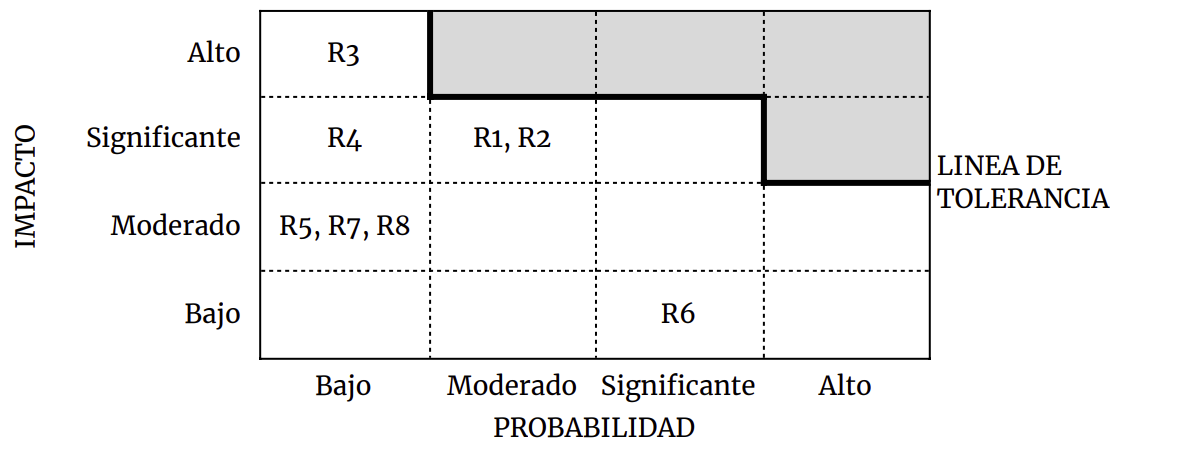
\includegraphics[width=12cm]{./img/spm/risk.matrix.png}
            \caption{Matriz de priorización de riesgos}
            \label{fig:riskmatrix}
        \end{figure}

\newpage
    \subsection{Riesgos identificados}
    \label{sec:riesgos.identificados}
        A continuación se clasifican los riesgos que pueden tener un impacto sobre el proyecto:
        %t1
        \begin{table}[H]
        \centering
        \begin{tabular}{|l|c}
        \hline
        \textbf{Riesgo}               & \multicolumn{1}{r|}{R-01}                                             \\ \hline
        \textbf{Descripción}          & \multicolumn{1}{X|}{El desarrollador puede enfermar debido a las  condiciones externas.}
        \\ \hline
        \textbf{Impacto}              & \multicolumn{1}{r|}{SIGNIFICANTE}                                             \\ \hline
        \textbf{Probabilidad}         & \multicolumn{1}{r|}{MODERADA}                                         \\ \hline
        \textbf{Plan de mitigación}   & \multicolumn{1}{X|}{Evitar acciones que atenten contra la salud. }
        \\ \hline
        \textbf{Plan de contingencia} & \multicolumn{1}{X|}{Trabajo desde casa.}
        \\ \hline
        \end{tabular}
        \caption{Riesgo 01 - Enfermedad}
        \label{table:riskill}
        \end{table}
        % t2
        \begin{table}[H]
        \centering
        \begin{tabular}{|l|c}
        \hline
        \textbf{Riesgo}               & \multicolumn{1}{r|}{R-02}                                             \\ \hline
        \textbf{Descripción}          & \multicolumn{1}{X|}{Mala planificación del proyecto.}
        \\ \hline
        \textbf{Impacto}              & \multicolumn{1}{r|}{SIGNIFICANTE}                                             \\ \hline
        \textbf{Probabilidad}         & \multicolumn{1}{r|}{MODERADA}                                         \\ \hline
        \textbf{Plan de mitigación}   & \multicolumn{1}{X|}{Reuniones cada dos semanas de seguimiento }
        \\ \hline
        \textbf{Plan de contingencia} & \multicolumn{1}{X|}{Aumentar el tiempo de trabajo hasta alcanzar lo planeado.}
        \\ \hline
        \end{tabular}
        \caption{Riesgo 02 - Planificación incorrecta}
        \label{table:malaplanif}
        \end{table}
        % t3
        \begin{table}[H]
        \centering
        \begin{tabular}{|l|c}
        \hline
        \textbf{Riesgo}               & \multicolumn{1}{r|}{R-03}                                             \\ \hline
        \textbf{Descripción}          & \multicolumn{1}{X|}{Pérdida del trabajo elaborado.}
        \\ \hline
        \textbf{Impacto}              & \multicolumn{1}{r|}{ALTO}                                             \\ \hline
        \textbf{Probabilidad}         & \multicolumn{1}{r|}{BAJA}                                         \\ \hline
        \textbf{Plan de mitigación}   & \multicolumn{1}{X|}{Utilización de varios servicios de control de versiones. }
        \\ \hline
        \textbf{Plan de contingencia} & \multicolumn{1}{X|}{Recuperar versiones más recientes.}
        \\ \hline
        \end{tabular}
        \caption{Riesgo 03 - Pérdida del trabajo}
        \label{table:riskperdida}
        \end{table}
        % t4
        \begin{table}[H]
        \centering
        \begin{tabular}{|l|c}
        \hline
        \textbf{Riesgo}               & \multicolumn{1}{r|}{R-04}                                             \\ \hline
        \textbf{Descripción}          & \multicolumn{1}{X|}{Caída de los servidores que alojan el servicio.}
        \\ \hline
        \textbf{Impacto}              & \multicolumn{1}{r|}{SIGNIFICANTE}
        \\ \hline
        \textbf{Probabilidad}         & \multicolumn{1}{r|}{BAJA}                                         \\ \hline
        \textbf{Plan de mitigación}   & \multicolumn{1}{X|}{ Usar servidores que aseguren un mínimo de disponibilidad. }
        \\ \hline
        \textbf{Plan de contingencia} & \multicolumn{1}{X|}{ Despliegue automático cuando el servidor arranque }
        \\ \hline
        \end{tabular}
        \caption{Riesgo 04 - Caída de los servidores}
        \label{table:riskperdida}
        \end{table}
        % t5
        \begin{table}[H]
        \centering
        \begin{tabular}{|l|c}
        \hline
        \textbf{Riesgo}               & \multicolumn{1}{r|}{R-05}                                             \\ \hline
        \textbf{Descripción}          & \multicolumn{1}{X|}{Rotura del equipo del dispositivo}
        \\ \hline
        \textbf{Impacto}              & \multicolumn{1}{r|}{MODERADO}                                             \\ \hline
        \textbf{Probabilidad}         & \multicolumn{1}{r|}{BAJA}                                         \\ \hline
        \textbf{Plan de mitigación}   & \multicolumn{1}{X|}{ Disponer de un mínimo de dos dispositivos. }
        \\ \hline
        \textbf{Plan de contingencia} & \multicolumn{1}{X|}{Comprar otro dispositivo.}
        \\ \hline
        \end{tabular}
        \caption{Riesgo 05 - Rotura de dispositivo}
        \label{table:riskrotura}
        \end{table}
        % t6
        \begin{table}[H]
        \centering
        \begin{tabular}{|l|c}
        \hline
        \textbf{Riesgo}               & \multicolumn{1}{r|}{R-06}                                             \\ \hline
        \textbf{Descripción}          & \multicolumn{1}{X|}{ Desconexión de la red WIFI del hogar. }
        \\ \hline
        \textbf{Impacto}              & \multicolumn{1}{r|}{BAJO}                                             \\ \hline
        \textbf{Probabilidad}         & \multicolumn{1}{r|}{SIGNIFICANTE}                                         \\ \hline
        \textbf{Plan de mitigación}   & \multicolumn{1}{X|}{ Conexión a la red a través de tarjeta SIM. }
        \\ \hline
        \textbf{Plan de contingencia} & \multicolumn{1}{X|}{ Recarga del saldo de la tarjeta SIM a través de Internet. }
        \\ \hline
        \end{tabular}
        \caption{Riesgo 06 - Desconexión de la red. }
        \label{table:riskdisconn}
        \end{table}
        % t7
        \begin{table}[H]
        \centering
        \begin{tabular}{|l|c}
        \hline
        \textbf{Riesgo}               & \multicolumn{1}{r|}{R-07}                                             \\ \hline
        \textbf{Descripción}          & \multicolumn{1}{X|}{Privatización de algún servicio.}
        \\ \hline
        \textbf{Impacto}              & \multicolumn{1}{r|}{MODERADO}                                             \\ \hline
        \textbf{Probabilidad}         & \multicolumn{1}{r|}{BAJA}                                         \\ \hline
        \textbf{Plan de mitigación}   & \multicolumn{1}{X|}{ Implementación del software adaptativa a cualquier servicio, para poder ser sustituído.
        
        Conocimiento del funcionamiento de otros servicios alternativos. }
        \\ \hline
        \textbf{Plan de contingencia} & \multicolumn{1}{X|}{ Sustitución del servicio.}
        \\ \hline
        \end{tabular}
        \caption{Riesgo 07 - Privatización de algún servicio. }
        \label{table:riskpriv}
        \end{table}


    \newpage
    \subsection{Riesgos acontecidos}
    
        Durante el transcurso del proyecto se pudo observar la aparición de ciertos riesgos:
        
        \begin{enumerate}
        
        \item \textbf{Riesgo 01 - Enfermedad}
        
        Descrito en la tabla \ref{table:riskill}, el desarrollador del sistema enfermó durante el último tramo del año.
        
        Este riesgo produjo un retraso de dos semanas en la elaboración del proyecto que el desarrollador tuvo que recuperar quitándose horas de sueño, ya que compartía este proyecto con otro trabajo externo.
        
        \item \textbf{Riesgo 02 - Mala planificación del proyecto}
        
        Descrito en la tabla \ref{table:malaplanif}, al utilizarse una planificación del proyecto mediante un modelo incremental, no se tuvo en cuenta el tiempo necesario para la escritura de la documentación formal, manteniendo una documentación informal a modo de cuaderno de bitácora donde se iban narrando los hechos.
        Este modelaje incremental hizo que se desarollasen más funciones de las que se esperaban en un principio, por lo que el periodo de escritura de la documentación aumentó notablemente, retrasando como consecuencia la finalización total del proyecto.
        
            \item \textbf{Riesgo 07 - Privatización de servicios}
            
        Descrito en la tabla \ref{table:riskpriv}, ocurrió cuando la plataforma de nuestro asistente inteligente fue comprada por Sonos. 
        
        A fecha de 31 de Enero de 2020, Snips Seeed privatizó sus servicios, bloqueando las funciones y el acceso a entrenamientos de nuestro asistente. Pese a tener analizado como posible riesgo la privatización de algún servicio, no se esperaba que la privatización fuese del asistente en general, ya que se analizó su modelo de negocio, donde se podía observar que tenía una fuerza para posicionarse como una de las primeras potencias en el mundo de los asistentes virtuales en los años venideros, ya que era el único asistente virtual capaz de trabajar sin una conexión fija a Internet. 
        
        Sonos vió también ese potencial y quiso hacerlo suyo, comprando la compañía para poseer la mejor baza de entre todos los asistentes con el fin de convertirse en los próximos años en uno de los líderes de este sector tecnológico.
        
        Gracias al plan de contingencia, y a la elaboración de un sistema que no dependa de ningun servicio específico, sino que todos los servicios implementen las funciones que el sistema requiera, el asistente podrá ser sustituido por otro de los nombrados anteriormente, posicionándose como mejor opción el asistente de Mycroft, descrito en el apartado \ref{Microft} del documento.
        
        
        \end{enumerate}

\newpage
\section{Costes}

    Para poder dar un valor monetario al proyecto hay que tener en cuenta sus costes, siendo tanto costes económicos como costes de desarrollo para poder ser realizado.

\begin{enumerate}
    \item \textbf{Duración estimada del proyecto} \label{duracion_proyecto}
    
El proyecto descrito en el presente documento es un proyecto relativo a un Trabajo de Fin de Grado (TFG), por lo tanto su estimación de horas de elaboración deberán corresponder con el coste de horas estimadas en cuanto al valor hora-credito de la carrera.

Según la documentación proporcionada por la Universidad de Valladolid~\cite{hxc}, cada crédito tiene una estimación de trabajo de 25 horas, y un TFG tiene asignado una cuantía de 12 créditos.

Por tanto, el trabajo estimado para la elaboración de un TFG es:

\begin{center}
    \textit{12 créditos * 25horas/crédito = 300 horas}
\end{center}

    \item\textbf{ Coste de personal:}
    
El salario medio para un desarrollador junior en España que todavía no tiene el título está, en el momento en el cual se está escribiendo el presente documento, en \textit{18966euros/año}~\cite{salario-junior}, y calculando que al año se hacen unas 1826 horas de trabajo de media, este desarrollador junior debería cobrar aproximadamente:

\begin{center}
    \textit{18966euros/1año * 1año/1826horas = 10,38euros/hora}
\end{center}

Teniendo en cuenta que la elaboración del proyecto tiene una estimación de 300 horas, el coste de personal será de:

\begin{center}
    \textit{10,38 euros/hora * 300 horas = 3116 euros}
\end{center}

    \item \textbf{ Coste del equipo: }
    
Para el desarrollo del proyecto se necesita la adquisición de dos dispositivos completos.

El coste del kit que proporciona la plataforma de Snips Seeed es de 115 euros por cada dispositivo, por lo que sería necesaria la inversión de:

\begin{center}
    \textit{115 euros/dispositivo * 2 dispositivos = 230 euros}
\end{center}

    \item \textbf{Coste de suministros}
    
    La duración del proyecto a desarrollar por el desarrollador, teniendo en cuenta que realice una jornada de 8 horas al día, será:
    
\begin{center}
    \textit{1826 horas/año / 12 meses/año = 154 horas/mes}
    
    \textit{300 horas/tfg / 154 horas/mes = 1,9480 meses/TFG}
\end{center}

    Como el gasto en suministros son cuotas mensuales, se aproxima a 2 meses de trabajo completo la resolución del TFG.
    
    El coste medio de consumo de suministros contando el acceso a internet y el consumo de la luz suma una cuantía de 25 euros al mes. Por tanto, el coste de suministros, sería de:
\begin{center}
    \textit{2 meses/TFG * 25 euros/mes = 50 euros/TFG}
\end{center}
    
\end{enumerate}

Teniendo en cuenta, que todo proyecto tiende a retrasarse, como indica el libro estandarte de la gestión de poyectos software~\cite{spm}, entre un 8\% y un 10\%, el coste total deberá ser recalculado, siendo la suma de todos los costes:

\begin{center}
    \textit{3116 + 230 + 50 = 3396 euros}
    
    \textit{3396 euros * 10\%  = 3735 euros}
\end{center}

El coste para la elaboración del proyecto, será por tanto la cuantía de \textbf{3608 euros}.



\chapter{Diseño}
\label{cap.diseño}
\subsection{Diagrama de casos de uso}

\subsection{Definición de casos de uso}

\subsection{Matriz de aproximación con requisitos}

\chapter{Implementación}\label{cap.implementation}
\section{Planteamiento}
Una buena realización de un proyecto comienza con un buen diseño inicial en el que se establecen las bases para un desarrollo correcto.

Este proyecto puede ser dividido en 3 subproyectos, donde cada subproyecto tendrá una arquitectura diferente debido a las necesidades que requiere su implementación.

El primer subproyecto es el asignado a la implementación de un software que será desplegado en el dispositivo y que permita la conexión con el servidor, aceptando la manipulación del propio dispositivo de manera remota.

El segundo subproyecto corresponderá con el propio sistema alojado en el servidor, al que llamaremos backend, el cual tendrá acceso a una base de datos y servirá una API REST para permitir una comunicación entre los dispositivos y los administradores.

El tercer subproyecto corresponde con el desarrollo de un sitio web, al que se llamará frontend, el cual permite el acceso a los administradores para el control y gestión de los dispositivos, al igual que para consultar las estadísticas.

\section{Arquitectura}
\subsection{Dispositivo}

En cuanto a la arquitectura final del dispositivo, no va a ser especificada ya que el presente proyecto no se adentra en la implementación del asistente, sino que pone las pautas y los protocolos mediante los cuales el asistente podrá comunicarse con el servidor.

Para poder mostrar estas pautas se ha implementado un controlador de pruebas, que será explicado junto a los casos de uso del dispositivo, pudiendo permitir posteriormente el desarrollo del asistente virtual inteligente con cualquiera de los métodos existentes.

\subsection{BackEnd} \label{arch-be}

Como se ha nombrado anteriormente, el sistema desarrollado en la parte del servidor deberá servir una API REST, de modo que la arquitectura elegida para la implementación del backend es una arquitectura REST, la cual se basa en ofrecer unos end-points desde los cuales se trata la información almacenada en el sistema.

Para una mejor implementación de esta arquitectura, se estructura el sistema bajo la Clean Architecture~\cite{clean-arch-book}, de modo que se permite el desarrollo del sistema en una organización formada por capas, donde el acceso a la siguiente capa es lineal, evitando dependencias cruzadas que perjudiquen la escalabilidad del sistema.

\begin{figure}[h!]
    \centering
    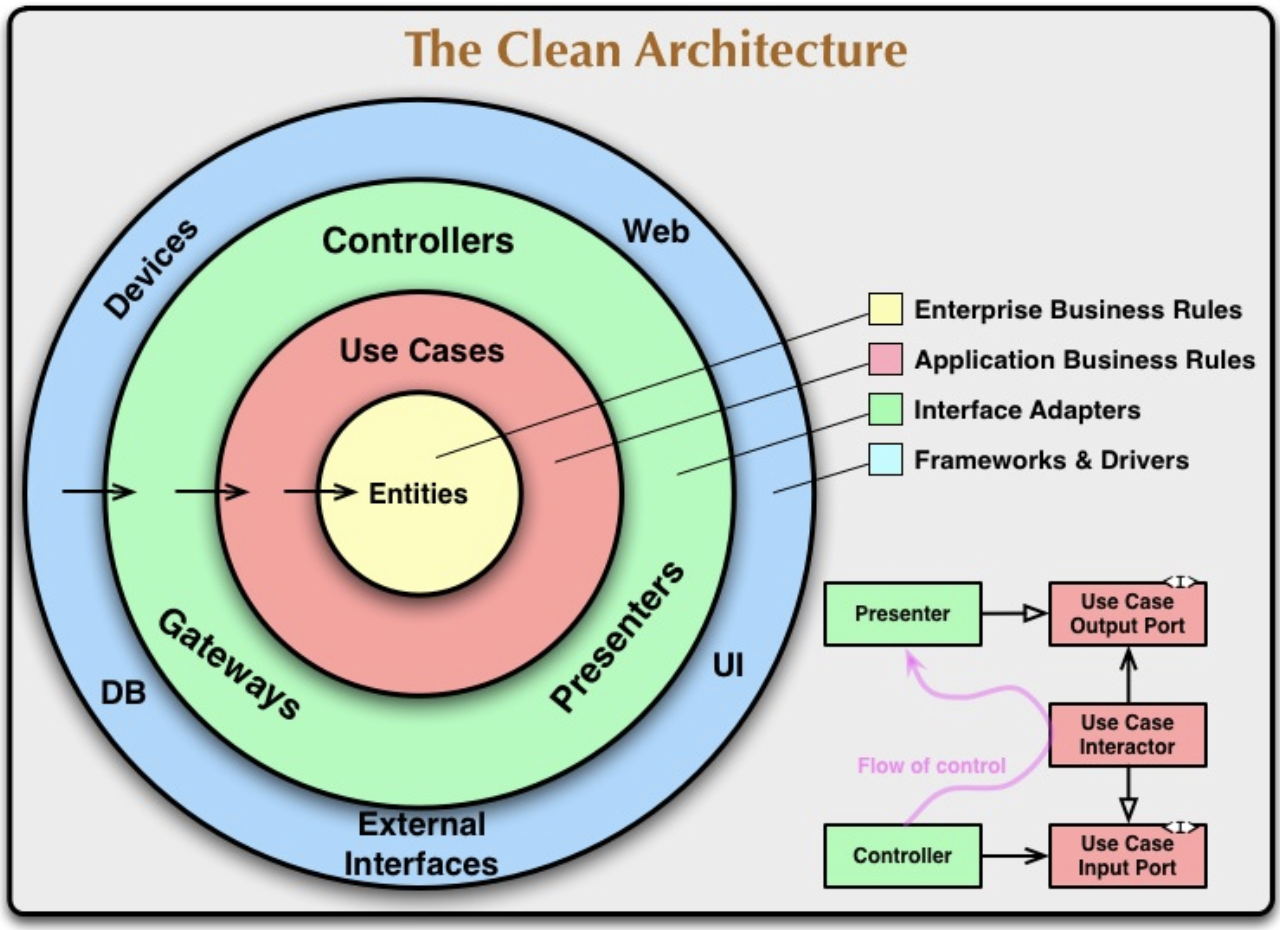
\includegraphics[width=7cm]{./img/arch/cleanarch.png}
    \caption{The Clean Architecture, Robert C. Martin~\cite{clean-arch-book}}
    \label{fig:cleanarch}
\end{figure}

\subsection{FrontEnd}

El sitio web a desarrollar para la administración del sistema se construye a partir del framework javascript de VueJS, como ya se ha mencionado anteriormente en el apartado \ref{Vue}.

VueJS propone una arquitectura MVVM~\cite{mvvm}, en la cual el diseño del sistema se basa en el desarrollo de múltiples componentes: Un componente es una unidad que dispone de su propio sistema de vista-presentador, teniendo una interfaz gráfica implementada en HTML + CSS, que efectúa un comportamiento a través de funciones JavaScript.

Esta modularidad interna basada en componentes debe seguir unas pautas~\cite{vuecomp} para sacar el máximo rendimiento de estos, al igual que para poder en un futuro remplazar o eliminar los componentes creados por otros que se ajusten a los nuevos requisitos sin perjudicar el resto de ellos.

Los datos que se manejan en la web aparecen en la vista de forma dinámica, de manera que es el presentador quien los puede variar.


\section{Implementación}
\subsection{Dispositivo}

El prototipo, al conectarse a una red eléctrica será el que inicie el asistente, al igual que dejará corriendo en segundo plano el subproyecto que hemos desarrollado con el fin de poder controlar y monitorizar el propio dispositivo.

    \subsubsection{Naturaleza del controlador}
    
        El monitoreo y control remoto de un dispositivo plantea el siguiente dilema: cómo invertir los roles para que un cliente haga de servidor recibiendo información, mientras el servidor hace de cliente mandando a este peticiones.
        
        Para resolver esta adversidad se toma una visión general del proyecto:
        \begin{enumerate}
            \item El dispositivo informa cada cierto tiempo de que sigue encendido.
            \item El servidor proporciona una API REST.
        \end{enumerate}
        
        Como bien se sabe, los operaciones básicas de una API REST son \textit{GET, POST, PUT y DELETE}, de modo que si se hace una petición \textit{GET} para informar sobre su conexión activa a la red eléctrica, se puede aprovechar por parte del servidor esta llamada para meter un mensaje específico en el cuerpo de la respuesta: este mensaje específico será el que propicie que se realice una acción en el dispositivo.
        
        De este modo el servidor podría manejar el dispositivo, monitorizándolo o pidiendo que haga acciones de manera remota, pudiendo tratarse por ejemplo de una tarea cuya finalidad sea que el asistente inicie una conversación con el usuario final en caso de que haya habido un accidente, de manera que se le pueda ayudar.
        
        Este planteamiento en cuanto a la naturaleza del controlador y su modo de uso parece factible, pero tiene la pega de la usabilidad, ya que si el dispositivo tiene una configuración de mandar su estado cada 24 horas, el control del dispositivo se demoraría demasiado, y aquí entra en juego la siguiente técnica:
        
        Se puede configurar en el propio dispositivo que las 24 horas que pasa entre aviso y aviso se obtengan a partir de un fichero de configuración, que permita la variación de estas 24 horas.
        También, en segundo plano, se puede configurar que a ciertas horas, el dispositivo disminuya su periodo de aviso, coincidiendo con unas ciertas horas relativas a la jornada laboral del admnistrador del sistema, de modo que este pueda mandarle una primera tarea que sea otra reducción del periodo de aviso, por ejemplo a 10 segundos, permitiendo una comunicación síncrona más pareja a una comunicación real, y permitiendo un envío posterior de tareas al dispositivo que se realizarían en un espectro corto de tiempo.
        
        En la figura \ref{fig:prototype-flow} se puede observar el flujo de estados propuesto e implementado en este proyecto con el fin de poder controlar y monitorizar el dispositivo.
        
        \begin{figure}[h!]
            \centering
            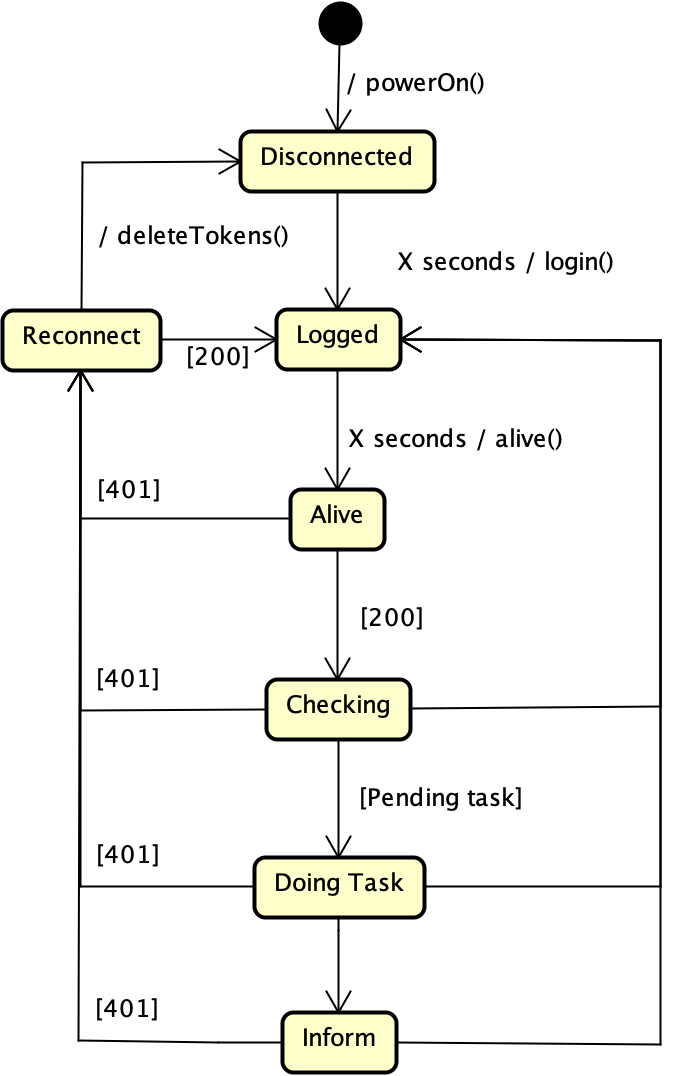
\includegraphics[width=7cm]{./img/state/prototype-flow.png}
            \caption{Flujo de estados del dispositivo}
            \label{fig:prototype-flow}
        \end{figure}
    
    \subsubsection{Desarrollo}
        Una vez planteada al teoría de cómo debe funcionar el asistente, toca ponerse con la práctica y demostrar que se puede formar un sistema que funcione y sea escalable.
        
        Para ello, se establece un espacio de trabajo dentro del dispositivo, el cual se vincula con un proyecto alojado en un servicio de control de versiones.
        De esta manera, se permite la posibilidad de actualizar las acciones del dispositivo con tan solo realizar una acción \textit{pull} del repositorio de origen.
        
        %% Sistema de arranque
        \textit{\textbf{Sistema de arranque}}
        
        El sistema implementado se ejecutará en el momento en el que se ejecute la clase \textit{Main.py}, que intenta iniciar sesión con el servidor a través del método \textit{signin()} de un objeto obtenido a través de la clase \textit{Login.py}.
        En el momento de instanciación del objeto \textit{login}, su constructor obtiene la dirección MAC del dispositivo, almacenándola en: 
        \begin{center}
        \textit{./cache/macfile.txt}
        \end{center}
        
        Esta dirección MAC propia y única para cada dispositivo, será utilizada como identificador en los credenciales a la hora de identificarse contra el servidor.
        La contraseña, será una encriptación de la dirección MAC que se obtiene simultáneamente en el constructor.
        
        Si se consigue iniciar sesión, se almacenan los tokens tanto en el objeto instanciado, como en el siguiente fichero externo:
        \begin{center}
        \textit{./cache/tokens.json}
        \end{center}
        
        Este almacenamiento externo permite su utilización a futuros programas que requieran los tokens para realizar peticiones contra el servidor. Continuando con el método el cual inició sesión, este devuelve un booleano, \textit{true}, desbloqueando un semáforo del \textit{main} que permite el envío al servidor del estado actual del dispositivo, a través de un método perteneciente a un objeto de tipo \textit{Alive.py}, el cual devuelve también otro booleano, que será \textit{false} en caso de que no se lleve la acción correctamente a cabo, cerrando el semáforo.
        
        Tras la implementación de este flujo de estados se ha podido comprobar la perfecta sincronía con el servidor, permitiendo proceder al diseño de un sistema que acepte la implementación de tareas.
        
        %% sistema de tareas
        \textit{\textbf{Sistema de tareas}}
        
        En el momento en el cual se hace la petición de \textit{/alive}, existen tres posibles respuestas por parte del servidor:
        \begin{enumerate}
            \item \textit{HTTP Status Code 200}: indica que la petición ha sido correcta.
            \item \textit{HTTP Status Code 300}: indica que la petición ha sido correcta, pero que hay múltiples respuestas, indicando al sistema del dispositivo que debe extraer la información que contiene el mensaje. En este mensaje, se incluye una lista de tareas pendientes del dispositivo:
            
            \newpage            
        \begin{lstlisting}
        [{
            "id" : "task identifier",
            "device" : "device identifier",
            "event" : "TAREA",
            "by" : "who ordered this",
            "at" : "when it was ordered"
        }]
        \end{lstlisting}
        
        
            \item \textit{HTTP Status Code 401}: indica que el token ha dejado de ser válido, por lo que se debería volver a iniciar sesión, o refrescar el token. Como un token de acceso tiene establecido por razones de seguridad un tiempo de validez de 30 minutos, y el dispositivo en principio realizará la petición de mostrar que sigue activo cada 24 horas, no se ve necesaria la implementación en el dispositivo de un método que refresque el token, ya que produciría un aumento del consumo de datos, al refrescar constantemente un token al que no va dar uso.
            
        \end{enumerate}
        \label{seq:received300}
        
        Una vez recibida una respuesta de tipo \textit{HTTP Status Code 300}, se procede a analizar las tareas pendientes que están en el cuerpo del mensaje. Para ello, se procede a ejecutar siempre la primera de la lista gracias a que han sido devueltas por orden de asignación desde el servidor.
        Analizando los campos de la tarea, vemos que dispone de campo llamado \textbf{event}, el cual indica el nombre de la tarea a realizar.
        
        El nombre de la tarea es único, y debe ser una palabra sin espacios, permitiendo utilizarlo como palabra clave.
        Gracias a esta palabra clave, se puede pedir al dispositivo que ejecute la tarea concreta, y para ello administramos el sistema de ficheros de modo que siga la siguiente estructura:
        
        \begin{center}
            \textit{./task/TAREA/}
        \end{center}
        y dentro de ese directorio, debe haber un script, el cual ejecute la tarea específica:
        
        \begin{center}
            \textit{./task/TAREA/init.sh}
        \end{center}
        
        \begin{figure}[h!]
            \centering
            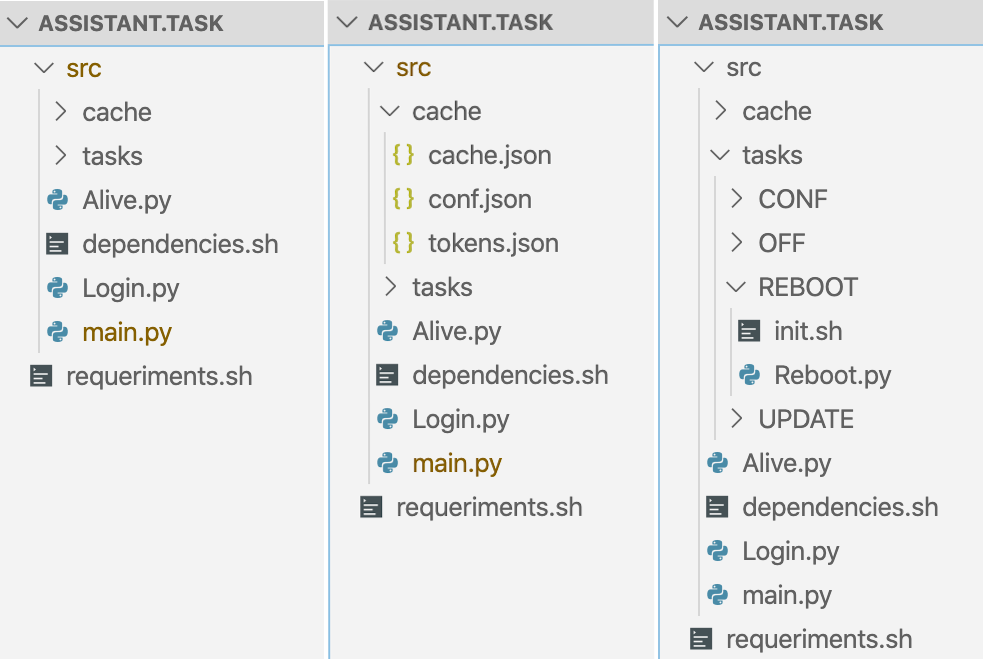
\includegraphics[width=10cm]{./img/arch/device/src.task.png}
            \caption{Contenido global del repositorio}
            \label{fig:src.task}
        \end{figure}
        
        Este script, puede llamar a otros programas o a otros scripts, de modo que se permite la realización de cualquier evento configurado.
        
        Una vez se tiene esta estructura implementada, como se puede observar en la figura \ref{fig:src.task}, tan solo hay configurar que al recibir como respuesta del servidor un código 300, se ejecute el script que está almacenado en la dirección obtenida al sustituir el nombre de la tarea, por ejemplo, \textbf{REBOOT}, en la ruta base:
        
        \begin{lstlisting}
            sh ./task/REBOOT/init.sh
        \end{lstlisting}
        
        Como se puede observar, este método de organización de tareas posibilita la fácil implementación de nuevas tareas sin poner en peligro las ya creadas, ya que únicamente se necesita crear un directorio nuevo por cada nueva tarea, y un script que inicie las acciones a realizar.
        
        %% estructura global
        
        
        
        %% inicio automático
        \textit{\textbf{Inicio automático}}
        
        Ya se tiene una configuración válida para el dispositivo, pero hay que poder asegurar su buen despliegue e inicio al reiniciar el dispositivo, de modo que se pueda tener como un valor seguro que, si un usuario reinicia la máquina físicamente, este dispositivo será capaz de iniciar el sistema ahora creado para poder monitorizarlo y controlarlo.
        
        Entonces, para la configuración del espacio de trabajo se proporciona un script que permite la configuración del dispositivo en caso de ser la primera vez que se utiliza ese dispositivo, por si no se han cargado bien los servicios.
        
        En dicho script, almacenado como \textit{requirements.sh}, se establecen dos pasos claves del proyecto:
        
        \begin{enumerate}
            \item La configuración para el inicio automático del sistema de control remoto del dispositivo a través de la herramienta de \textit{crontab}~\cite{crontab} que proporcionan los sistemas Unix.
            
        \begin{lstlisting}
        # configure scheduled task
        (crontab -l ; echo "@reboot sleep 60; cd /home/pi/assistant.task/src/ ; python /home/pi/assistant.task/src/assistant-alive.py & > home/pi/assistant.task/src/cache/logfile.txt") | crontab -
        \end{lstlisting}
        
        De este modo, se abre el fichero de configuración de \textit{crontab} en el cual se plasma qué es lo que se desea que se ejecute en cada reinicio, como indica la etiqueta \textit{@reboot}.
        Si se presta atención al script, se solicita una espera de 60 segundos a partir del reinicio del dispositivo, y el motivo por el cual se establece ese tiempo es para permitir que el dispositivo pueda configurar su conexión a internet y levantar previamente todos sus servicios antes de que el sistema aquí descrito arranque, evitando posibles interferencias que no permitiese arrancar de la manera correcta, como puede ser una mala obtención de la dirección MAC de la tarjeta de red.
        
        \item El script de lo requisitos ejecuta otro script, el de la instalación de las dependencias, el cual permite la instalación de las librerías de python requeridas para el correcto funcionamiento del dispositivo.
        
        \begin{lstlisting}
        # install python dependencies
        sudo sh ./src/dependencies.sh
        \end{lstlisting}
        
        De esta manera, se establecen las medidas y acciones necesarias, al igual que los scripts requeridos para poder asegurar el cumplimiento y buen funcionamiento del dispositivo aplicando los protocolos de comunicación descritos.
        
        \end{enumerate}


\subsection{BackEnd}

    \subsubsection{Introducción}

        Para el desarrollo del BackEnd se va a seguir la arquitectura descrita en el apartado \ref{arch-be}, de modo que a continuación se describirá cómo esa arquitectura ha sido implementada, con qué herramientas, y cuáles son las dependencias o servicios que posee.

    \subsubsection{Principios de diseño}
    
        Para un buen desarrollo de un sistema software se debe seguir los patrones de diseño, al igual que se deben aplicar los diferentes principios de diseño.
        
        A la hora del desarrollo, se ha considerado respetar los principios de diseño \textbf{SOLID}~\cite{clean-arch-book}:
        
        \begin{enumerate}
            \item Open-Closed Principle:
            
            Partimos de un lenguaje como Kotlin el cual toda clase de datos es cerrada en cuanto a extensión. De este modo, se ha asegurado que toda clase que se requiera como abierta lleva el operador \textit{open} con ella.
            
            \item Single responsability Principle:
            
            Se ha respetado que cada clase tenga únicamente una única función, dividiendo en varias toda clase que requiera más de una responsabilidad. Esto se ha podido asegurar a la hora de la implementación y segregación del sistema en servicios a la hora de acceder a la base de datos, al igual que en los múltiples controladores que posee el sistema con tal de acceder y realizar funciones diferentes.
            
            \item Liskov Substitution Principle:
            
            El principio de sustitución de Liskov nos dice que debemos perservar el funcionamiento de una interfaz o clase en el momento que la heredamos, de modo que una redefinición de un método debe poder cumplir los contratos. Este principio se ha complido a la hora de implementar los servicios, ya que se ha requerido que cumplan todos y cada uno de los requisitos impuestos en las interfaces de la capa de la lógica del sistema.
            
            \item Dependency Inversor Principle:
            
            El sistema ha sido implementado siguiendo el esquema de The Clean Arquitecture, como ya se ha nombrado anteriormente, de modo que los endpoint de la API Rest son quienes solicitan a los controladores la realización de cierto caso de uso.
            Los controladores, para la realización de estos casos de uso pueden requerir el acceso a servicios o repositorios externos. Para ello, cada controlador indica cuales son los servicios que va a necesitar, y si un servicio quiere servir al caso de uso, debe cumplir con los contratos establecidos en la interfaz pública del caso de uso.
            De esta manera, siguiendo todos los principios anteriores, se cumple este principio ya que si el servicio integra la interfaz, el servicio puede ser inyectado en el caso de uso, permitiendo una estanquedad de los controladores a los servicios externos, y con ello facilitanto el cambio de un servicio por otro sin que afecte al sistema, y cumpliendo así el principio de inversión de dependencia.
            Para la inyección de estas dependencias ha sido utilizado el framework de Koin, el cual ha sido explicado anteriormente en el apartado \ref{Koin}.
            
            \item Interface Segregation Principle:
            
            El principio de segregación de interfaces nos indica que una buena práctica se basa en contar con varias interfaces específicas de modo que se pueda utilizar una u otra en función del tipo de cliente.
            Esto se ha llevado a cabo a la hora de comprobación de credenciales, ya que se proporciona una interfaz u otra en función de si el token recibido viene por parte de un dispositivo, o de un administrador, pudiendo ambos iniciar sesión, pero ejecutándolo diferentes controladores.
            
        \end{enumerate}
        
        En cuanto a patrones de diseño, se han seguido en mayor medida los descritos a continuación gracias a haber aplicado los principios SOLID descritos anteriormente:
        
        La elaboración de un sistema por capas con una comunicación de dependencias lineal nos permite la utilización del \textbf{patrón fachada}, ya que para la conexión entre servicios y controladores hay una interfaz pública la cual limita el número y tipo de objetos que se mandan entre ambos, evitando una sobrecomunicación, al igual que una relación de dependencias circulares.
        
        Gracias a la aplicación de este patrón, se da cabida a la posibilidad de aplicación del \textbf{patrón adaptador}, permitiendo la creación de unas nuevas interfaces intermedias que adapten las interfaces públicas de los controladores a posibles futuros servicios que sustituyan a los actuales, sin necesidad de modificar el comportamiento de los controladores los cuales ya realizan los casos de uso, y asegurando entonces un aislamiento escalable.
        
        También, los servicios han servido de punto de acceso a la información de la base de datos gracias al uso del framework \textit{ExposedSQL}, de modo que ha intercambiado la información con los controladores a través de objetos, separando por tanto el acceso a la BBDD de la capa de negocio, aplicando por tanto el \textbf{patrón DAO} y posibilitando cambiar en un futuro el sistema de almacenaje de información sin que requiera un solo cambio en la capa de negocio del sistema.
        
        A la hora de mantener un registro de cómo está funcionando el sistema, se ha utilizado el \textbf{patrón Singleton} con el fin de obtener una instancia del objeto Logger, y con ello poder retransmitir logs desde cualquier punto del sistema sin requerir aumentar los recursos y evitando errores de interferencias por re-declaración. También, se ha aplicado este patrón para el acceso al \textit{TokenStore}, el cual almacena los tokens activos, y de esta manera permitir la comunicación entre el controlador de sesión con el servidor OAuth a través de la misma instancia, ya que al instanciar un nuevo objeto se perderían los tokens activos ya creados.
    
    \subsubsection{Servicios}
    
        Los servicios forman el acceso a la capa más externa según el esquema de \textit{The Clean Architecture}, y han sido implementados aceptando y cumpliendo las condiciones impuestas en las interfaces públicas de la capa de negocio.
        
        De esta manera, los servicios que requiere el sistema son los siguientes:
        \begin{enumerate}
            \item\textit{ConfService:}
            A través de este servicio se puede obtener cualquier configuración existente, ya sea de los dispositivos, de las localidades, o globales. También tiene la opción de marcar ciertas configuraciones como ya instaladas, crear nuevas, o borrarlas en función del identificador o de su estado.
            
            \item\textit{DeviceService:}
            Este servicio proporciona la información relativa a un dispositivo, siendo posible comprobar si un dispositivo existe en el sistema, comprobar las credenciales, crear uno nuevo, obtener todos, obtener el dispositivo asociado a un determinado usuario, asignar un dispositivo a un usuario concreto, o almacenar y recolectar los últimos estados del dispositivo.
            
            En este servicio se puede apreciar la utilidad de segregar el sistema en servicios, al igual que la inversión de dependencias, ya que se podría sustituir facilmente el servicio cambiando por tanto la manera en la que se registran los dispositivos, o cambiando la manera en la que se comprueban las credenciales, que en el caso de este sistema es mediante la encriptación de la dirección MAC, por otro tipo de comprobación sin alterar el funcionamiento de la capa de negocio, que seguiría aislada.
            
            \item\textit{IntentsService:}
            Permite almacenar las actividades realizadas en los dispositivos, es decir, la información relevante obtenida tras una comunicación \textit{máquina-usuario}. También permite obtenerlos, ya sea el último de una máquina, o una lista de los realizados por un dispositivo específico entre dos fechas.
            
            \item\textit{LocationService:}
            Ofrece la posibilidad de almacenar nueva localidades y luego recopilarlas ya sean todas, por código postal, o por provinicias.
            
            \item\textit{PeopleService}
            Relativo a los clientes que tendrán en su poder un dispositivo. Es útil para añadir personas y para obtenerlas después ya sean todas, o por su nif, o por código postal, al igual que poder obtener los datos sobre el dispositivo asignado para una persona en concreto.
            
            \item\textit{TaskService:} Controla la información almacenada sobre los eventos y tareas asignadas a dispositivos, de manera que permite la adición y obtención de eventos, al igual que de dispositivos. También permite la obtención de tareas pendientes de un dispositivo concreto, o la recolección de todas las tareas de un dispositivo concreto ocurridas en un rango de tiempo concreto.
            
            \item\textit{UserService:} Este servicio lleva la gestión de usuarios del sistema, es decir, de administradores del sistema, que son diferentes que los clientes de los dispositivos. Estos usuarios poseen una contraseña y el servicio ofrece la manera de verificar que sus credenciales son correctos.
            
        \end{enumerate}
    \subsubsection{Más a fondo}
    
    Debido a la complejidad del sistema, se ilustrará el diseño del sistema con varias figuras y sus explicaciones correspondientes con el fin de que el lector pueda comprender la implementación y replicarla en un futuro, al igual que pueda modificar lo que requiera, si en un futuro quiere tomar este documento como manual para una reimplementación del sistema.
    
    El backend estará estructurado en 3 capas:
    
    \begin{figure}[H]
    \centering
        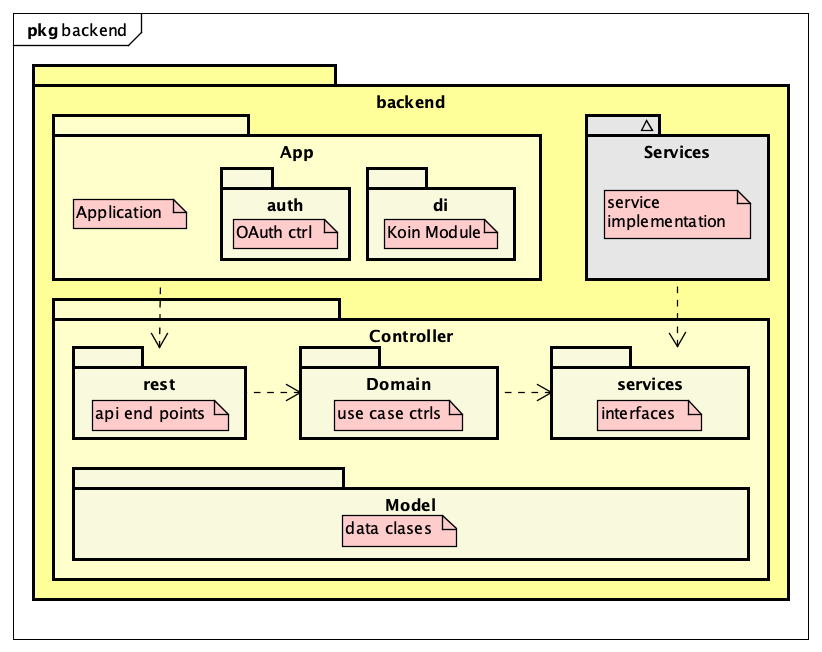
\includegraphics[width=10cm]{./img/arch/back/diagram.design.png}
        \caption{Diagrama de diseño}
        \label{fig:designdiagram}
    \end{figure}

    \begin{enumerate}
        \item \textbf{App:}
        Albergará la aplicación que iniciará el sistema, al igual que tendrá dos subdirectorios. El directorio \textit{auth} manejará la configuración sobre los tokens de acceso, y el directorio \textit{di} será el que contenga la configuración del inyector de dependencias, el cual se configura mediante la implementación de un módulo.
        
        \item \textbf{Controller:}
        Se asocia a la \textit{capa de negocio} del sistema, de modo que se puede considerar el componente aislado principal del sistema, ya que no depende de ninguna clase externa y proporciona modos mediante los cuales se puede acceder a su uso.
        Internamente, se puede observar el directorio \textit{rest}, el cual contiene los end-points del sistema, los cuales se explicarán más adelante. Otro de los directorios es el subdirectorio de \textit{Domain}, el cual contiene los controladores mediante los cuales se realizan los casos de uso. Estos controladores tienen la lógica del sistema, y para acceder a recursos externos como puede ser la base de datos u otros servicios externos, utilizan servicios externos inyectados a través del framework, siempre y cuando esos servicios externos utilicen las interfaces que proporcionan los controladores. El tercer directorio es el de \textit{services}, el cual contiene las interfaces requeridas por los controladores y consiguiendo con esto una inversión de dependencias, ya que de requerir un servicio por parte del controlador, se ha pasado a que el servicio requiera, para poder ser utilizado, la implementación de estas interfaces.
        
        Se puede observar un cuarto directorio, \textit{Model}, el cual contiene clases que serán utilizadas para el envío de datos entre las diferentes capas, evitando la utilización en esta capa de negocio de clases de datos externas que produzcan una dependencia.
        
        \item \textbf{Services:}
        Son los servicios externos que proporcionan información al sistema. Estos servicios deben implementar las interfaces de servicios que proporciona la capa de negocio. De este modo, si las implementan, pueden ser inyectados a través del inyector de dependencias.
    \end{enumerate}
    


    La aplicación que arranca el sistema y maneja toda la configuración es \textit{./src/app/Application.kt}.
    
    En cuanto a los endpoints del sistema, se pueden declarar en la propia aplicación, pero se considera buena-práctica el disgregarlos en diferentes módulos, agrupados por rutas o servicios similares, obteniendo así una mejor visibilidad y permitiendo un acceso intuitivo a la hora del desarrollo.
    
    A cada módulo de ruta se le otorga el acceso a los servicios necesarios que va a requerir los controladores. De este modo, al declarar los end-points se le proporcionan los servicios en su constructor, y se evita una dependencia directa de la capa de negocio con el framework elegido para inyectar esas dependencias, ya que las dependencias se inyectan en el módulo iniciador de la aplicación, el cual es externo a la capa de negocio, siguiendo manteniéndola aislada del exterior.
    
    En el siguiente diagrama se puede observar los 3 subpaquetes ya descritos anteriormente que conforman el sistema, al igual que las dependencias entre ellos: tanto el paquete \textit{App} como el paquete \textit{Services} dependen del paquete \textit{Controller}, el cual no depende de ningun otro y por tanto, está aislado de los cambios del exterior.
    
    \begin{figure}[H]
    \centering
    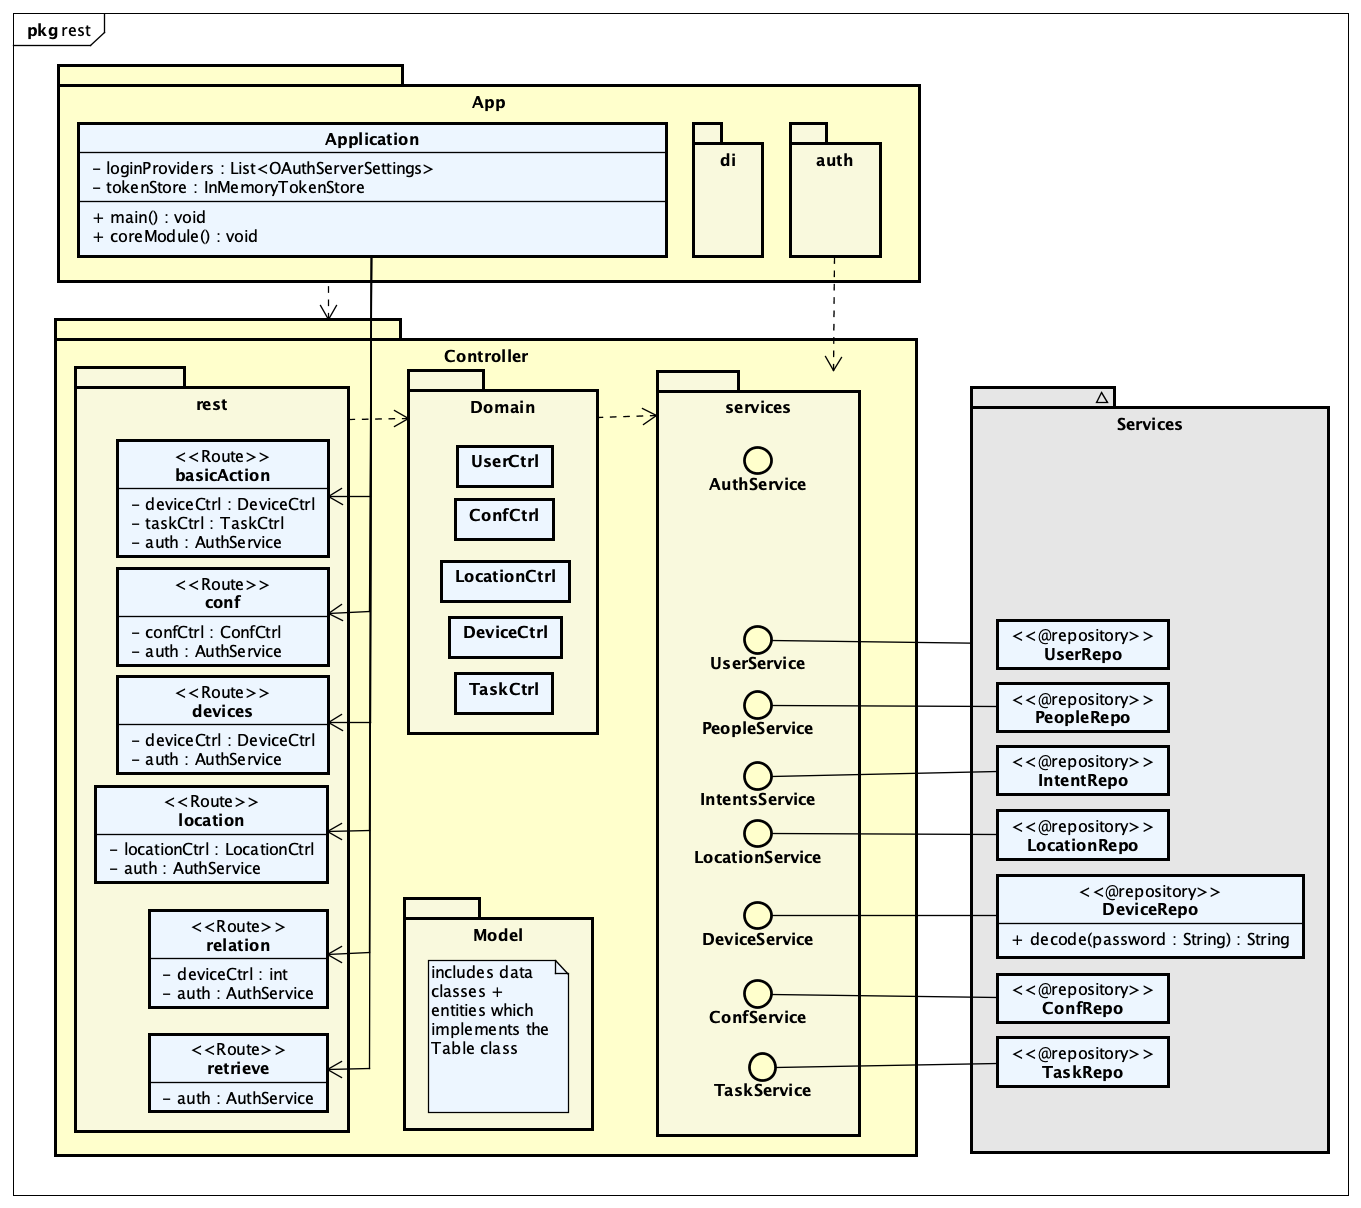
\includegraphics[width=14cm]{./img/arch/back/diag.class.2.png}
    \caption{Diagrama de Clases: General}
    \label{fig:diagram.app}
\end{figure}

    En la figura anterior se ha podido ver la estructura y dependencias de cada subpaquete de manera general.
    Ahora, se particularizará mostrando la estructura interna de cada uno de ellos, explicándo qué es y para qué se utiliza cada parte.
    
    Teniendo en cuenta la figura \ref{fig:dc.app}, podemos observar diferentes partes:
    
    Por un lado, tanto \textit{InMemoryIdentityCustom} como  \textit{InMemoryTokenStore}, que son modificaciones del framework OAuth que permiten la utilización del store de tokens fuera del framework, de modo que los tokens se puedan gestionar a través del sistema. Su instalación ya ha sido explicada en el apartado \ref{oauth20}, de modo que no se va a entrar ahora de nuevo.
    
    Una vez ya obtenido un acceso público de \textit{TokenStore}, este será gestionado únicamente desde el servicio creado para el control de tokens, \textit{TokenCtrl}, el cual implementa la interfaz \textit{AuthService}, permitiendo que este servicio sea inyectado en el sistema.
    
    Esta inyección se produce tras la implementación en \textit{Application} del módulo de dependencias creado con Koin, \textit{app.di.Module.myModule}, el cual también ha sido explicado cómo debe ser instalado en la aplicación en el apartado \ref{Koin}, al igual que el resto de servicios.
    
    La aplicación, por tanto, obtendrá los servicios inyectados y se los proporcionará a cada ruta, como se pueden observar en la figura \ref{fig:dc.app}, de modo que la capa de negocio ya dispondrá de los servicios para su uso, a través de las interfaces que había predefinido.

    \begin{figure}[H]
        \centering
        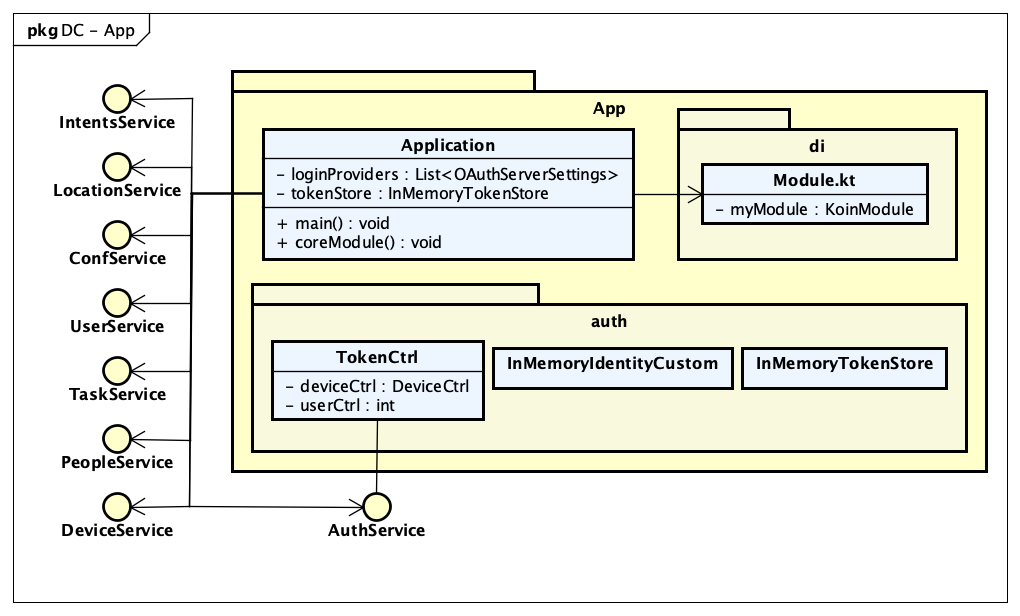
\includegraphics[width=14cm]{./img/arch/back/dc.app.png}
        \caption{Diagrama de Clases: App}
        \label{fig:dc.app}
    \end{figure}

    En cuanto a la capa de negocio expuesta en la \ref{fig:diagram.app} como \textit{Controller}, se puede observar que los paquetes \textit{Domain}, \textit{services}, y \textit{Model} no han sido explicados, por lo que se mostrará en las siguientes figuras su contenido.
    
    Se puede observar en la figura \ref{fig:dc.domain} que \textit{Domain} contiene el dominio de la aplicación, gestionando los controladores que hacen que se cumplan todos los casos de uso descritos anteriormente, almacenando toda la lógica del sistema.
    
    Cada controlador tiene atribuídas unas las dependencias, que están relacionadas con las interfaces descritas por esta capa de negocio, asegurando por tanto que no se va a tener que implementar ninguna operación externa.

    Las interfaces \textit{-descritas en la figura \ref{fig:dc.services}-} muestran las operaciones requeridas por los controladores, sirviendo de contrato para los servicios externos que quieran dar un uso futuro al sistema.
    
    \begin{figure}[H]
        \centering
        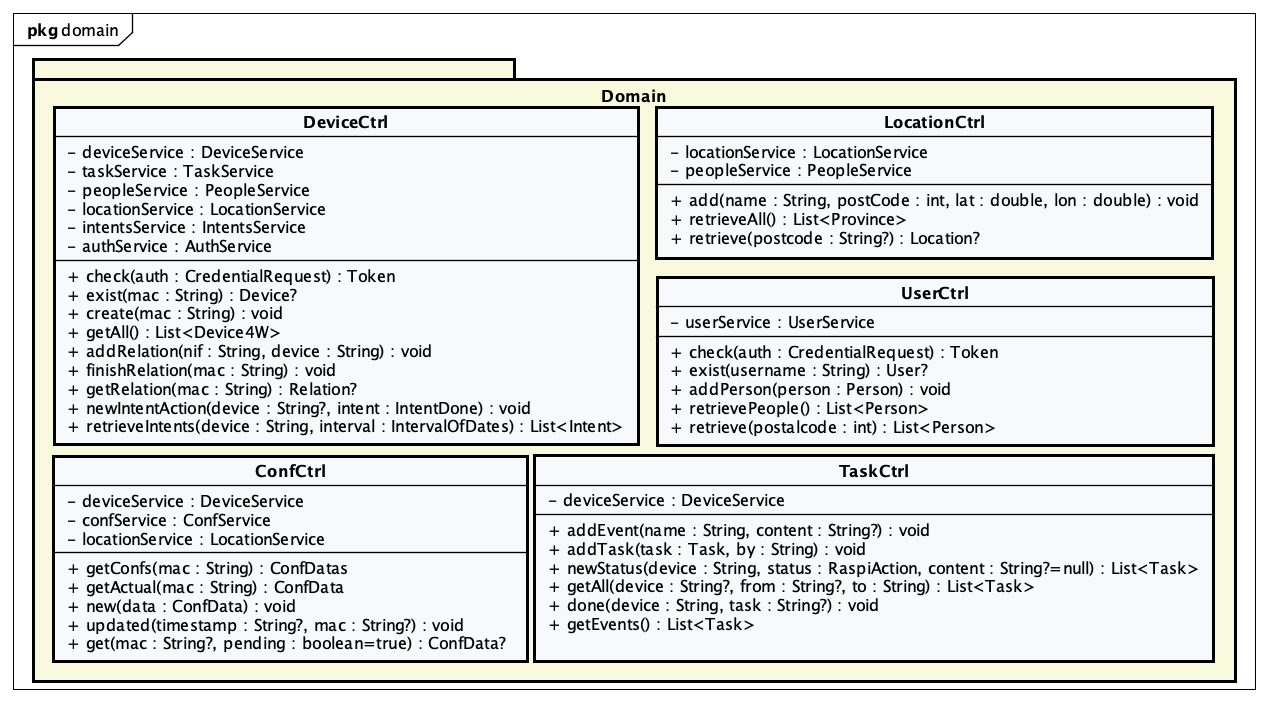
\includegraphics[width=13cm]{./img/arch/back/dc.domain.png}
        \caption{Diagrama de Clases: Domain}
        \label{fig:dc.domain}
    \end{figure}
        
    \begin{figure}[H]
        \centering
        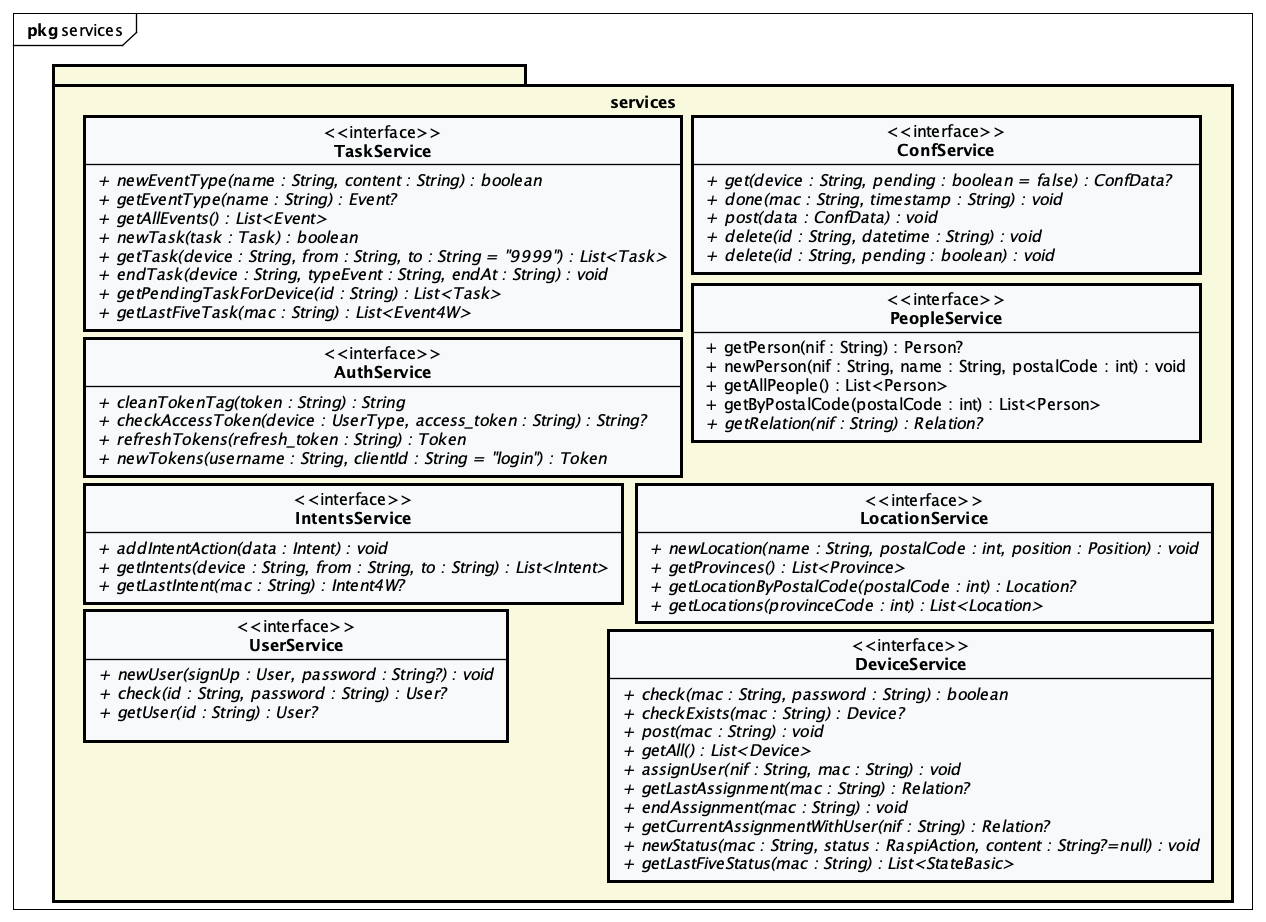
\includegraphics[width=14cm]{./img/arch/back/dc.services.png}
        \caption{Diagrama de Clases: Services}
        \label{fig:dc.services}
    \end{figure}

    Para la comunicación entre la capa de negocio con las otras capas, al igual que para la gestión de la información en comunicaciones internas se necesitan unas clases que sirvan para el envío de datos, favorenciendo y simplificando la comunicación.
    
    Estas clases, llamadas \textit{clases de datos}, son las mostradas a continuación en la figura \ref{fig:dc.model}.

    \begin{figure}[H]
        \centering
        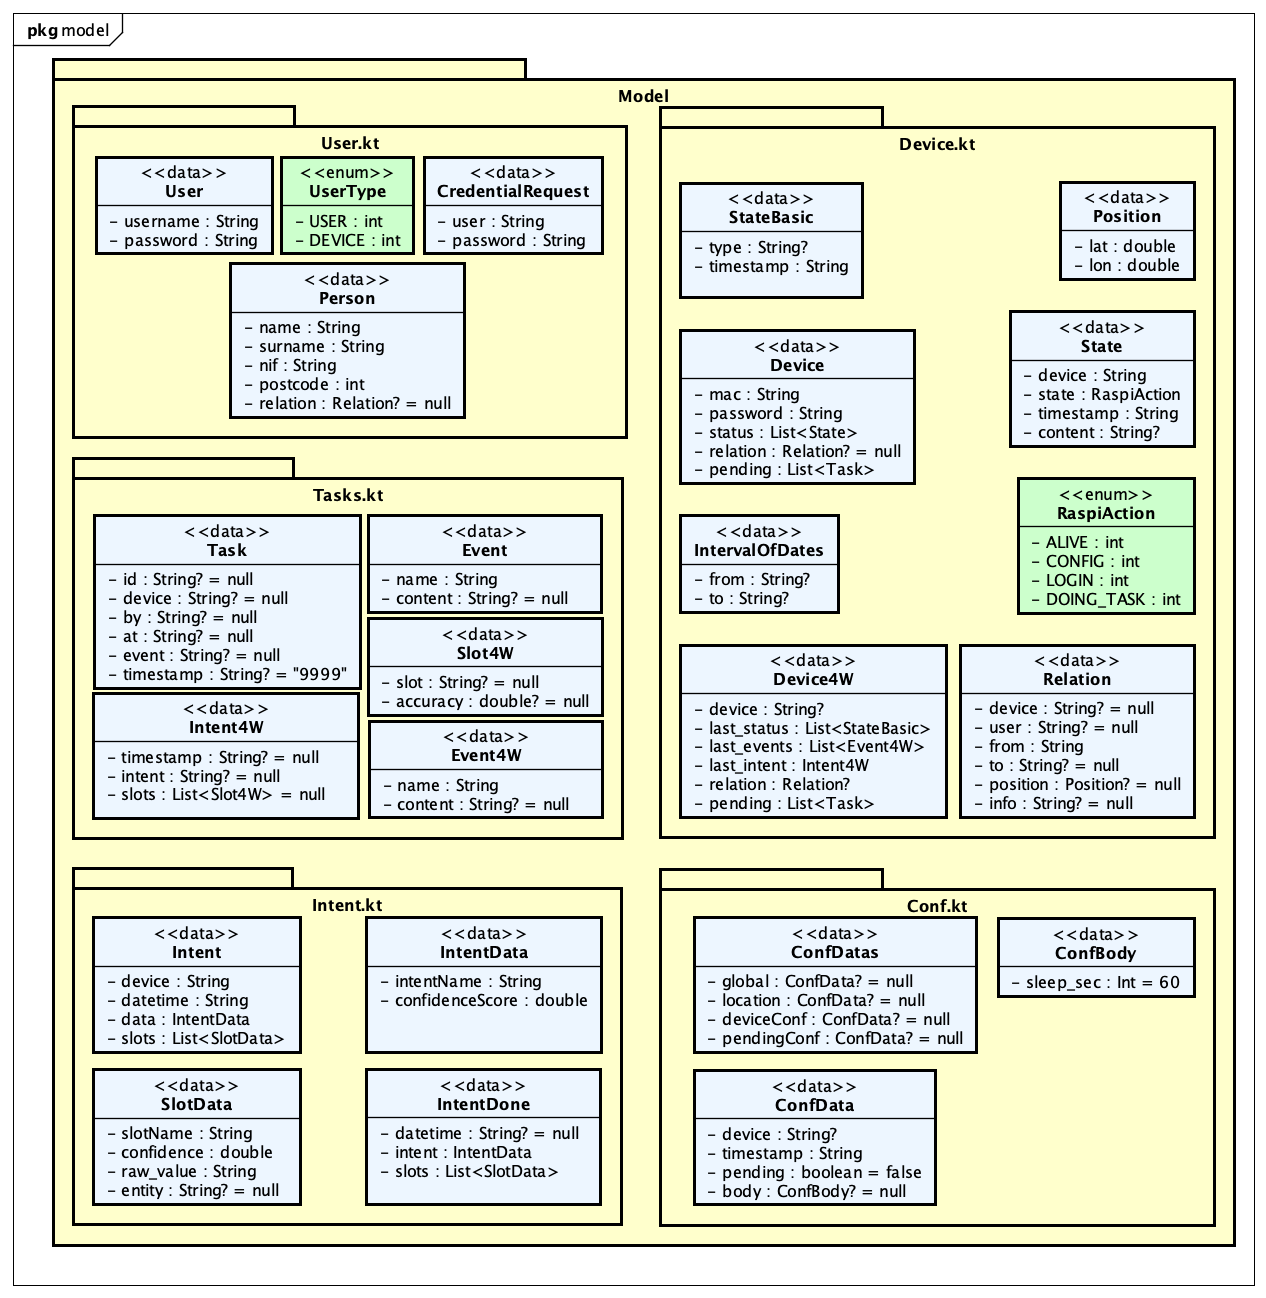
\includegraphics[width=14cm]{./img/arch/back/dc.model.png}
        \caption{Diagrama de Clases: Model}
        \label{fig:dc.model}
    \end{figure}


    \newpage
    \subsubsection{Diagrama Entidad-Relacion}
    
    En el siguiente diagrama, representado con la figura \ref{fig:d.er}, se puede observar cuales son las relaciones entre las distintas tablas que componen la base de datos, de modo que se aprecian las dependencias de claves que comparten entre si.
    
\begin{figure}[H]
    \centering
    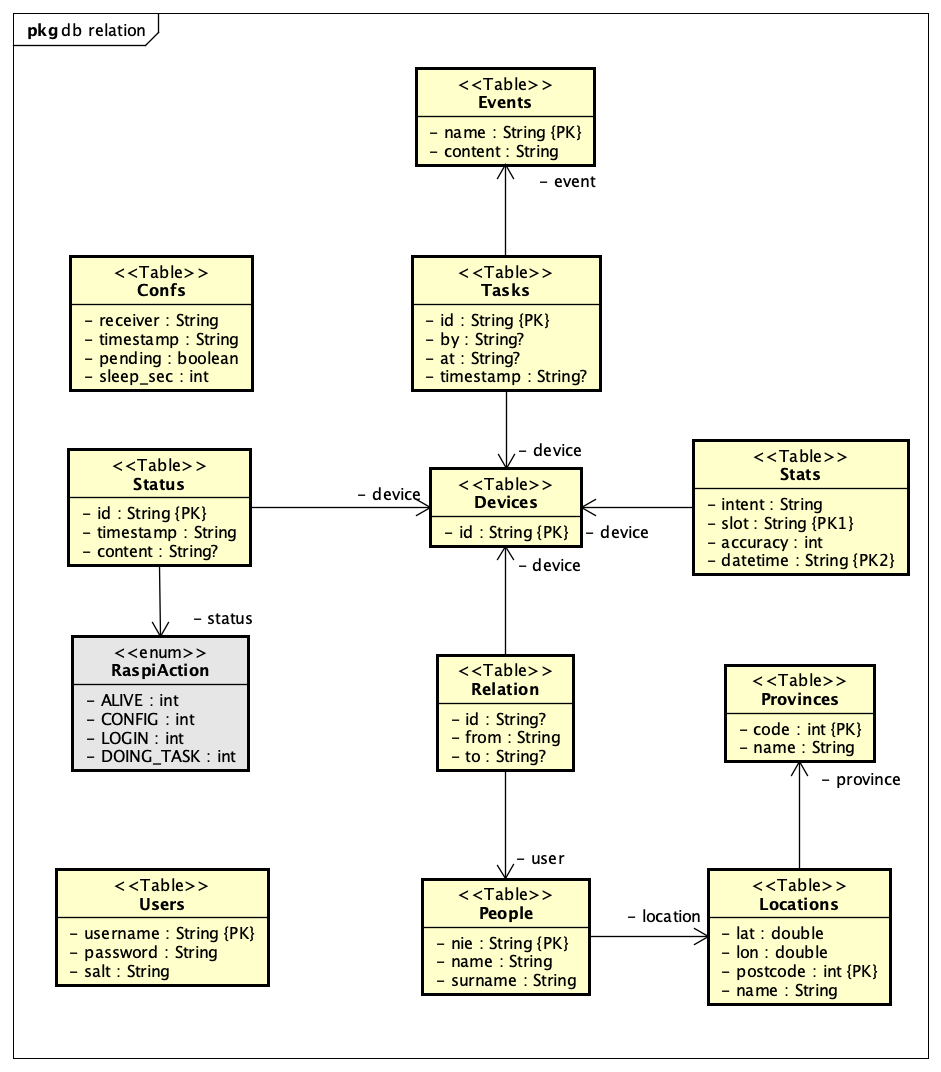
\includegraphics[width=14cm]{./img/arch/back/d.er.png}
    \caption{Diagrama Entidad-Relación}
    \label{fig:d.er}
\end{figure}

    \subsubsection{End-Points}
    \input{secciones/6implementacion/3impl/endpoints}
    
\newpage
\subsection{FrontEnd}

    \subsubsection{Estructura de directorios}
    La parte del sitio web del sistema se ha desarrollado con VueJS a través del instalador de gradle, lo que proporciona un sistema de directorios similar a cualquier otro proyecto de VueJS, de modo que es más simple entender el funcionamiento.

    \begin{figure}[H]
        \centering
        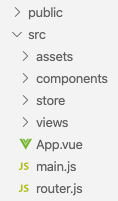
\includegraphics[width=3cm]{./img/web/web.dir.png}
        \caption{Estructura del FrontEnd: Model}
        \label{fig:web.dir}
    \end{figure}

En cuanto a una explicación rápida, el proyecto tendrá dos directorios sobre los que se trabaja, y que pueden observarse en la figura \ref{fig:web.dir}:
\begin{enumerate}
    \item \textbf{/public} el cual almacena el fichero \textit{index.html} del sistema, donde se pueden importar todos los script, al igual que almacena los posibles iconos del sistema, siendo de acceso público. En cuanto a la práctica, no se recomienda almacenar ahí ningún fichero de carácter sensible, ya que es de fácil acceso al público.
    
    \item \textbf{/src} contiene la lógica del sitio web, y funciona del siguiente modo:
    \textit{/src/main.js} carga la aplicación Vue, y al ser el módulo principal llevará el control de todas las peticiones que se realizan a la aplicación. Por ello, se ha instalado dentro un interceptor de peticiones, el cual añade el token de acceso al sistema en todas y cada una de ellas, al igual que lo refresca en caso de que se caduque.
    
    Este módulo por tanto carga la aplicación, \textit{App.vue}, la cual sirve de contenedor para mostrar todas las vistas posibles. Para mostrar estas vistas, se seleccionan a través del enrutador el cual está definido en \textit{/src/router.js}.
    Las vistas que pueden ser cargadas deben almacenarse en \textit{/src/views}, y son las que acceden a los datos de la aplicación. Los datos de la aplicación se pueden almacenar tanto en las propias vistas si solo son necesarios en esa vista, o en el controlador si se va a requerir compartir la información con otras vistas.
    
    Los controladores están en \textit{/src/store} y almacenan tanto la información generada por la aplicación, como la que obtienen de servicios externos.
    Para un desarrollo mejor estructurado de cada vista, el contenido puede ser dividido en componentes, de modo que cada vista sea un conjunto de cada uno de ellos y permitiendo exportar esos componentes una vez estén implementados a otras aplicaciones, al igual que pudiendo traer componentes externos.
    Estos componentes estarán en \textit{/src/components} y toda la información de la que puedan disponer será la generada por ellos mismos, o la información que se les ha introducido a través de atributos, pero nunca accederán al controlador del sistema.
    
    Se considera mala práctica que estos componentes accedan a métodos de sus padres, \textit{siendo el padre la vista que lo carga, o otro componente que lo cargue}, ya que crearía una dependencia que lo convertiría en componente no aislado, produciendo errores si se incluye en un nuevo padre que no implemente esos métodos, por lo que si se requiere llamar a un antecesor, lo recomendable sería la emisión de eventos, los cuales podrían ser recogidos y tratados por el padre.
    
    En cuanto a la inclusión de scripts externos para la mejora del sistema, pueden ser añadidos via instalación por comandos con \textit{npm}, o pueden ser descargados e incluídos en el directorio \textit{/src/assets}.
\end{enumerate}

    
    \subsubsection{ Diseño de interfaz }
    El diseño de la interfaz ha sido basado en la implementación de los requisitos del sistema que han sido definidos en el apartado \ref{req.fun}.

En cuanto a la interfaz de usuario, se ha buscado seguir los patrones de \textit{responsive web design}, permitiendo la adaptación del contenido de la página en función del dispositivo el cual la esté cargando, pudiendo ser tanto monitores de ordenadores, como tablets o smartphones.

\begin{enumerate}

    \item \textbf{Dashboard} %%% DASHBOARD
    
Se prediseñó un panel de dashboard en el cual los dispositivos apareciesen como recuadros de colores, que cambiasen su color en función del estado.
Al pulsar un color, se abriría una tarjeta en la cual aparecería la información relativa al dispositivo.

    \begin{figure}[H]
        \centering
        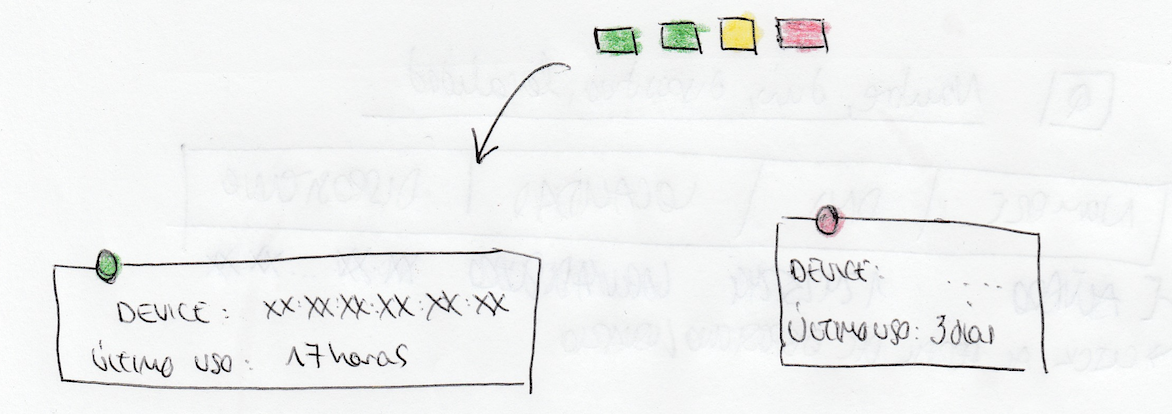
\includegraphics[width=10cm]{./img/web/devices/dev.pre.png}
        \caption{Dashboard: Planteamiento de diseño}
        \label{fig:devices.pre}
    \end{figure}

Finalmente, pese a  que esta opción permitía la visualización de cientos de dispositivos a la vez, no proporcionaba una buena identificación de qué recuadro era un dispositivo concreto, o cuánto tiempo exacto había pasado.
Por ello, se optó por mostrar directamente las tarjetas de los dispositivos, cambiando la forma en que aparecen los colores y haciéndola más fácil de comprender, localizar e identificar un dispositivo concreto.

En las siguientes figuras aparecen las posibles variaciones de las tarjetas.
    
    \begin{figure}[H]
        \centering
        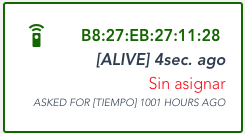
\includegraphics[width=4cm]{./img/web/devices/dev.green.png}
        \caption{Dashboard: Dispositivo en línea}
        \label{fig:web.dir}
    \end{figure}
    
    \begin{figure}[H]
        \centering
        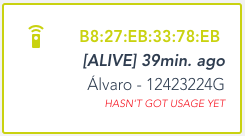
\includegraphics[width=4cm]{./img/web/devices/dev.greellow.png}
        \caption{Dashboard: Dispositivo reciente}
        \label{fig:web.dir}
    \end{figure}
    
    \begin{figure}[H]
        \centering
        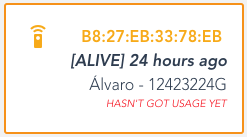
\includegraphics[width=4cm]{./img/web/devices/dev.orange.png}
        \caption{Dashboard: Dispositivo ausente}
        \label{fig:web.dir}
    \end{figure}
    
    \begin{figure}[H]
        \centering
        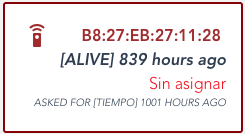
\includegraphics[width=4cm]{./img/web/devices/dev.red.png}
        \caption{Dashboard: Dispositivo posiblemente apagado}
        \label{fig:web.dir}
    \end{figure}
    
    \begin{figure}[H]
        \centering
        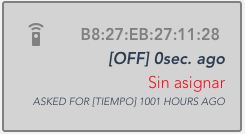
\includegraphics[width=4cm]{./img/web/devices/dev.grey.png}
        \caption{Dashboard: Dispositivo apagado por comando}
        \label{fig:web.dir}
    \end{figure}
    
    \begin{figure}[H]   
        \centering
        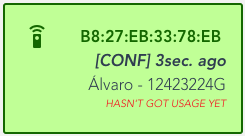
\includegraphics[width=4cm]{./img/web/devices/dev.doing.png}
        \caption{Dashboard: Dispositivo realizando tarea enviada}
        \label{fig:web.dir}
    \end{figure}
    
    En el dashboard, con el fin de poder localizar más rápidos los dispositivos que cumplan una serie de condiciones, se debe permitir un filtrado de ellos:
    \begin{enumerate}
        \item El dispositivo tiene un usuario asignado o no.
        \item Se ordenan por fecha de su última actividad, o por fecha de su última tarea.
        \item Ese orden es realizado de manera ascendente, o descendente.
    \end{enumerate}
    
    El panel que permitiese este filtrado fue prediseñado de manera simple en una ventana emergente que recibe el nombre de \textit{modal} en el mundo del desarrollo web, facilitando de manera simple y efectiva la realización, como se puede ver a continuación.
    
    \begin{figure}[H]   
        \centering
        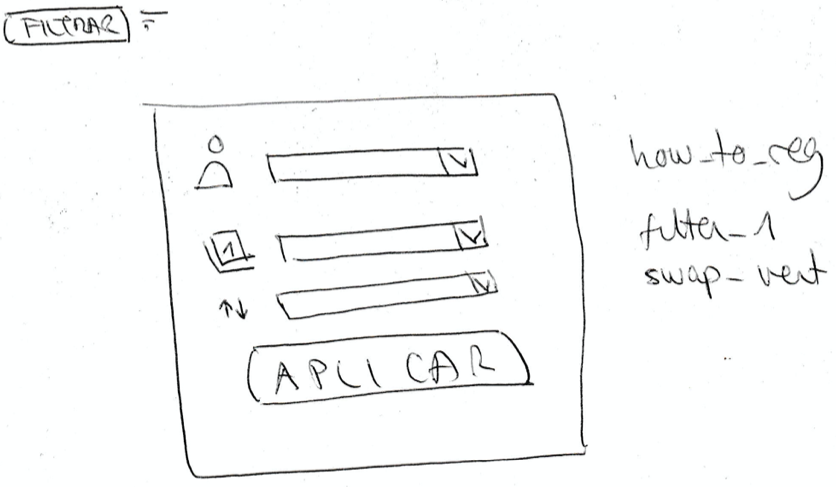
\includegraphics[width=7cm]{./img/web/devices/dev.filter.pre.png}
        \caption{Dashboard - Planteamiento del filtro de dispositivos}
        \label{fig:web.dir}
    \end{figure}
    
    El diseño final implementado no tuvo ningún cambio ya que el plantemiento del diseño cumplía con las expectativas, ofreciendo una satisfactoria experiencia de usuario.
    
    \begin{figure}[H]   
        \centering
        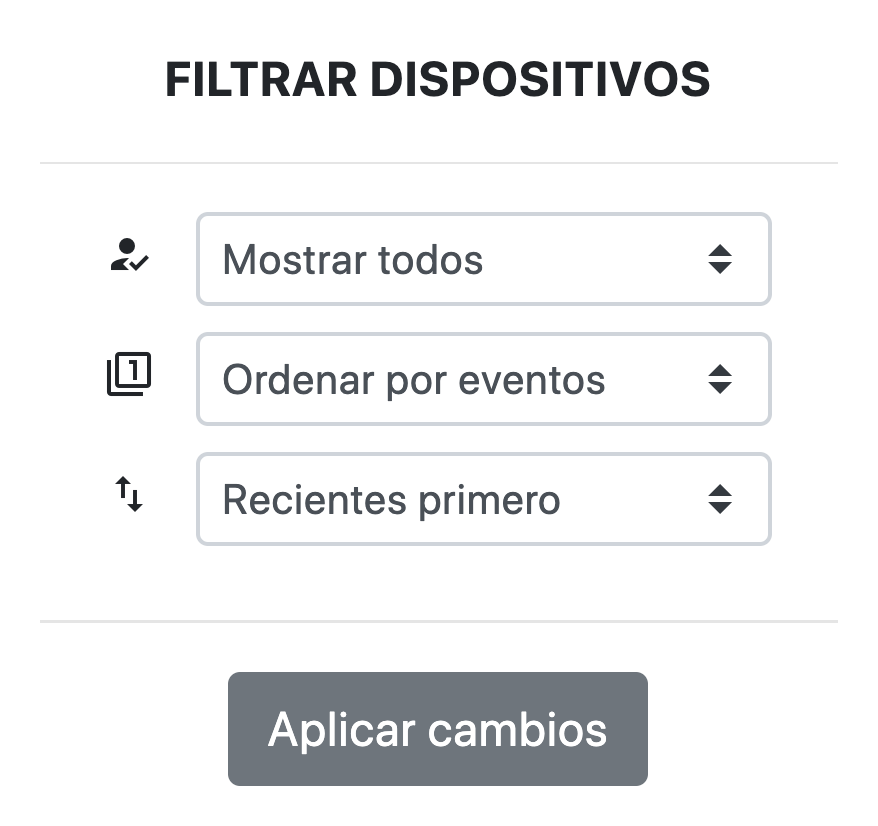
\includegraphics[width=8cm]{./img/web2/home.device.filter.png}
        \caption{Dashboard - Diseño final del filtro de dispositivos}
        \label{fig:web.dir}
    \end{figure}
    
    En cuanto a las tarjetas en las cuales aparece la información del dispositivo, deben permitir un acceso a la visualización de estadísticas, o a la selección rápida de tareas. También, debe permitir servir de punto base para acceder a otros servicios del sistema como puede ser la configuración de los parámetros del dispositivo.
    
    \begin{figure}[H]   
        \centering
        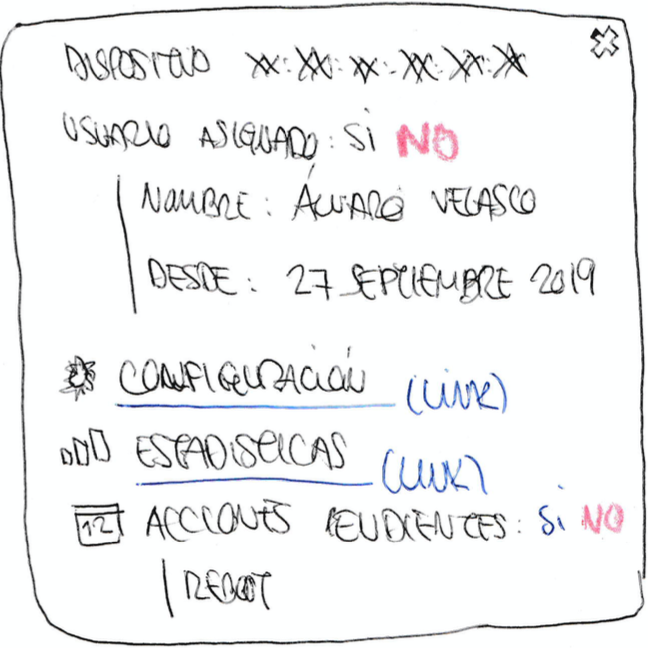
\includegraphics[width=7cm]{./img/web/devices/dev.quick.pre.png}
        \caption{Dashboard - Planteamiento de diseño de acciones rápidas.}
        \label{fig:web.dir}
    \end{figure}    
    
    \begin{figure}[H]   
        \centering
        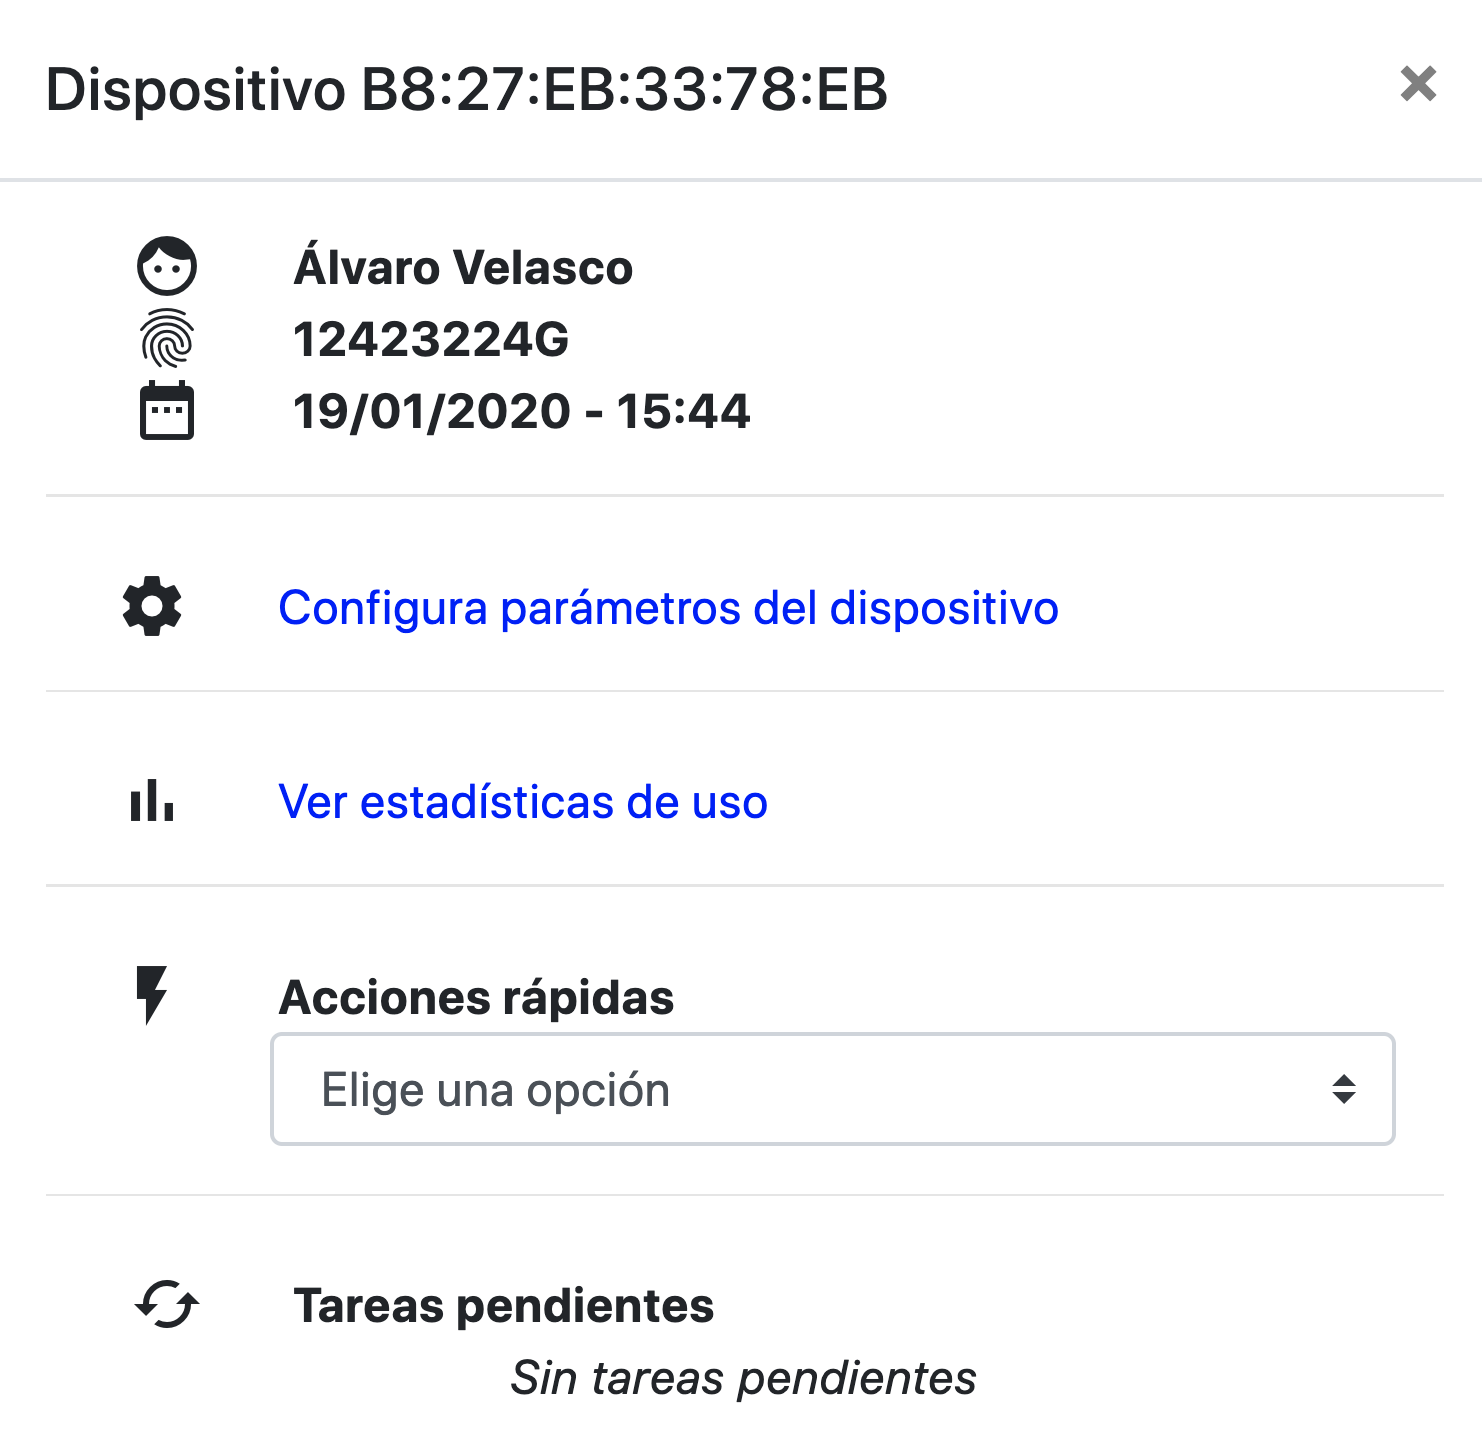
\includegraphics[width=9cm]{./img/web2/home.device.info.user}
        \caption{Dashboard - Diseño final de acciones rápidas: dispositivo asignado.}
        \label{fig:web.dir}
    \end{figure}
    
    \begin{figure}[H]   
        \centering
        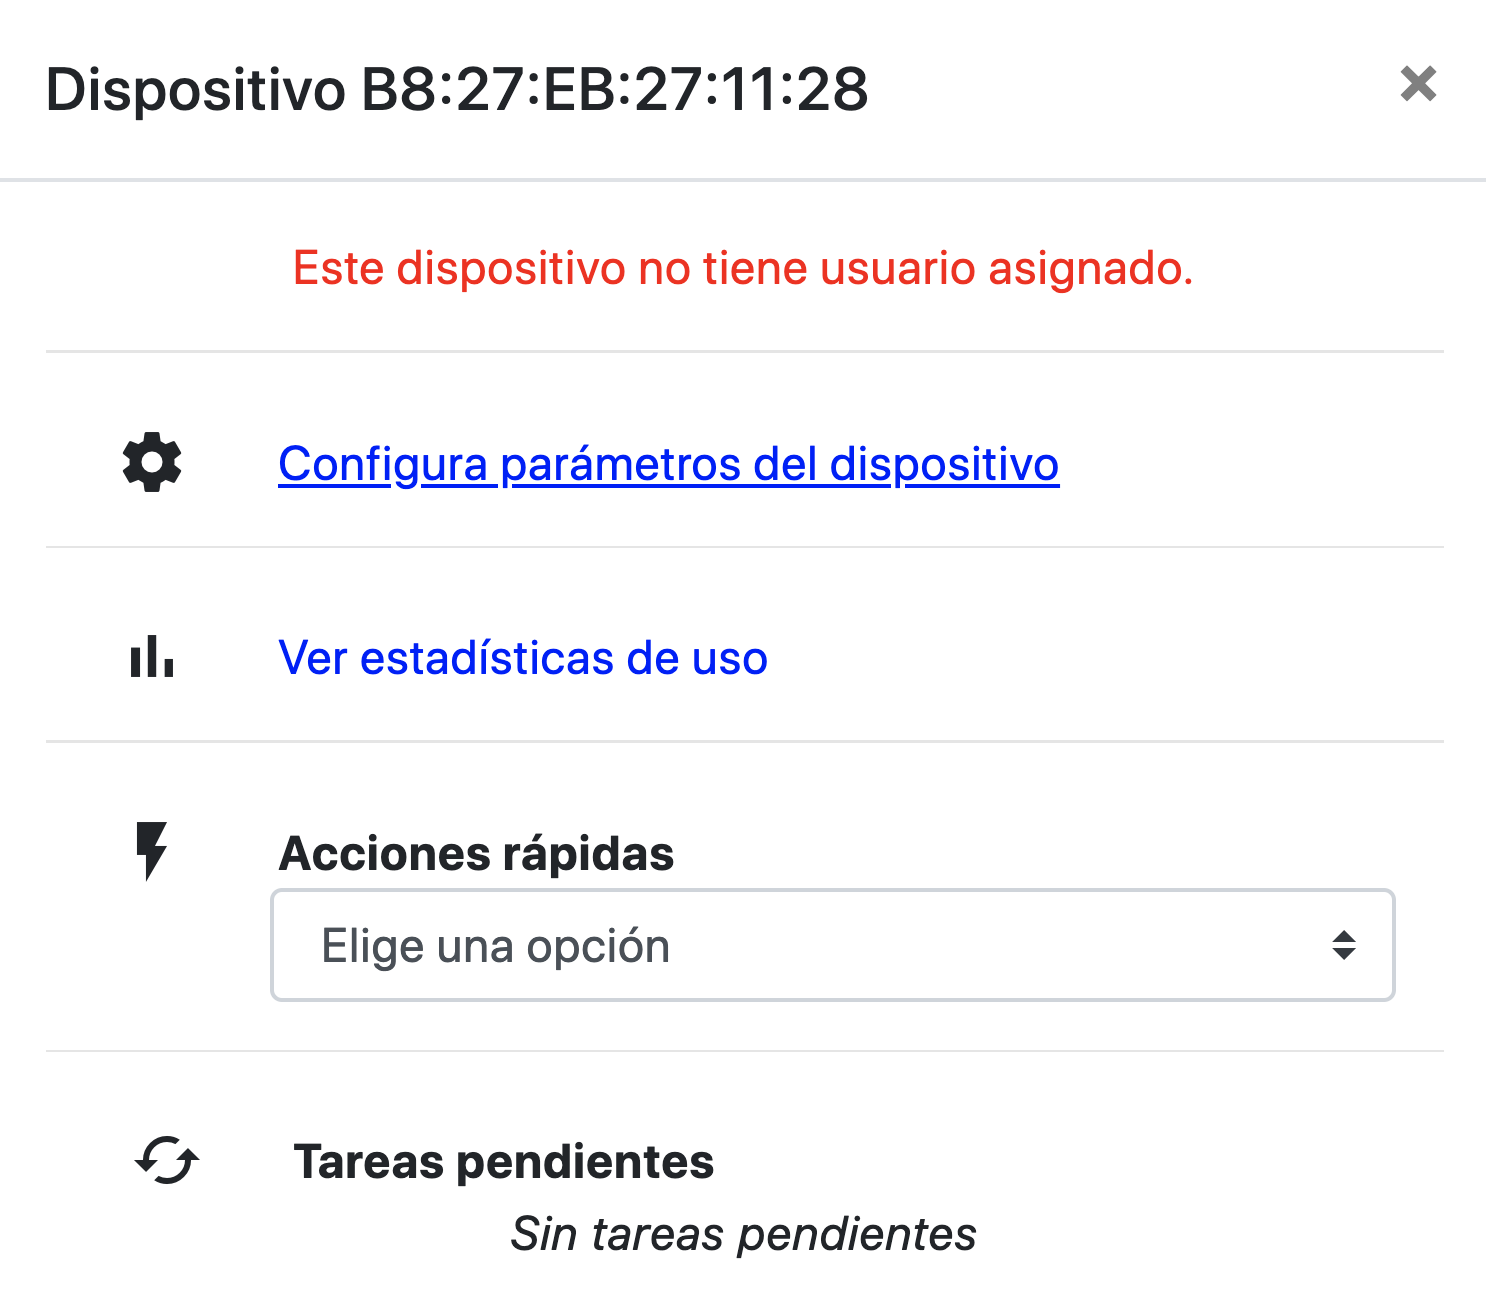
\includegraphics[width=9cm]{./img/web2/home.device.info}
        \caption{Dashboard - Diseño final de acciones rápidas: dispositivo sin asignar.}
        \label{fig:web.dir}
    \end{figure}
    
    
    \item \textbf{Localidades} %%% LOCALIDADES
    
    En esta sección se buscaba la posibilidad de ver una lista detallada de qué localidades estaban registradas en el sistema, al igual que cuántos dispositivos o personas estaban asocidados a cada localidad.
    
    Se contempló como buena idea en los diseños previos la posibilidad de una lista de provincias que contengan alguna localidad registrada mostrando las estadisticas generales, y que pulsando en ellas, se abriese la lista de localidades asociadas, con sus datos particulares.
    
    \begin{figure}[H]   
        \centering
        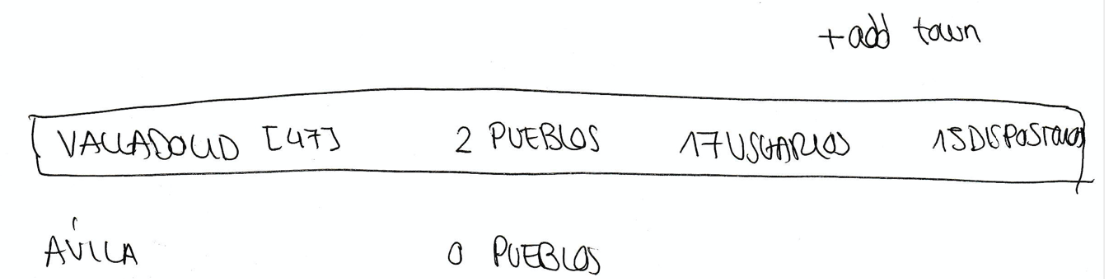
\includegraphics[width=11cm]{./img/web/locations/locations.closed.pre.png}
        \caption{Localidades - Planteamiento de lista: agrupado por provincias.}
        \label{fig:web.dir}
    \end{figure}
    
    \begin{figure}[H]   
        \centering
        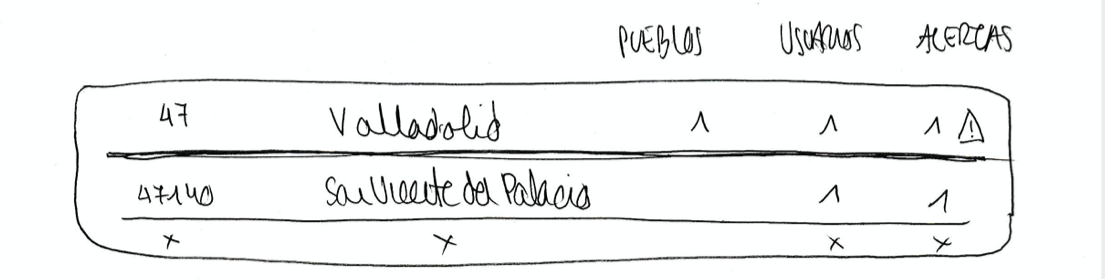
\includegraphics[width=11cm]{./img/web/locations/locations.opened.pre.png}
        \caption{Localidades - Planteamiento de lista: despliegue de provincia.}
        \label{fig:web.dir}
    \end{figure}
    
    \begin{figure}[H]   
        \centering
        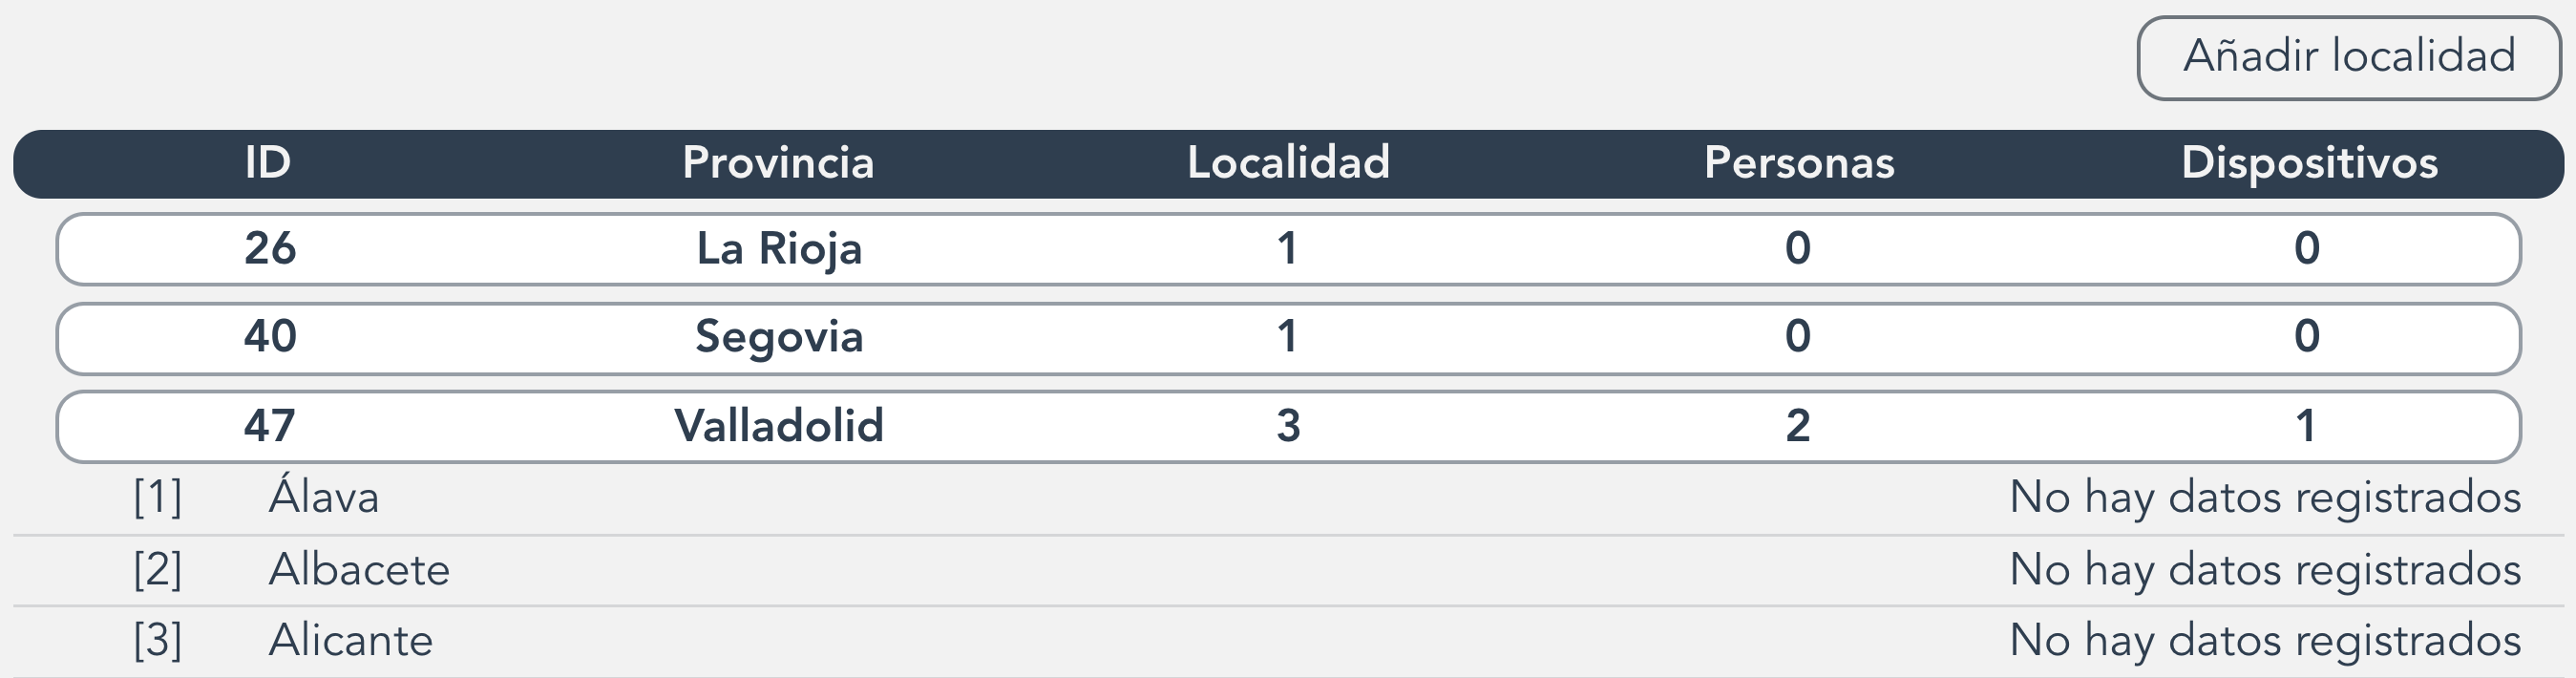
\includegraphics[width=11cm]{./img/web2/locations.table.png}
        \caption{Localidades - Diseño final de lista: agrupado por provincias.}
        \label{fig:web.dir}
    \end{figure}
    
    \begin{figure}[H]   
        \centering
        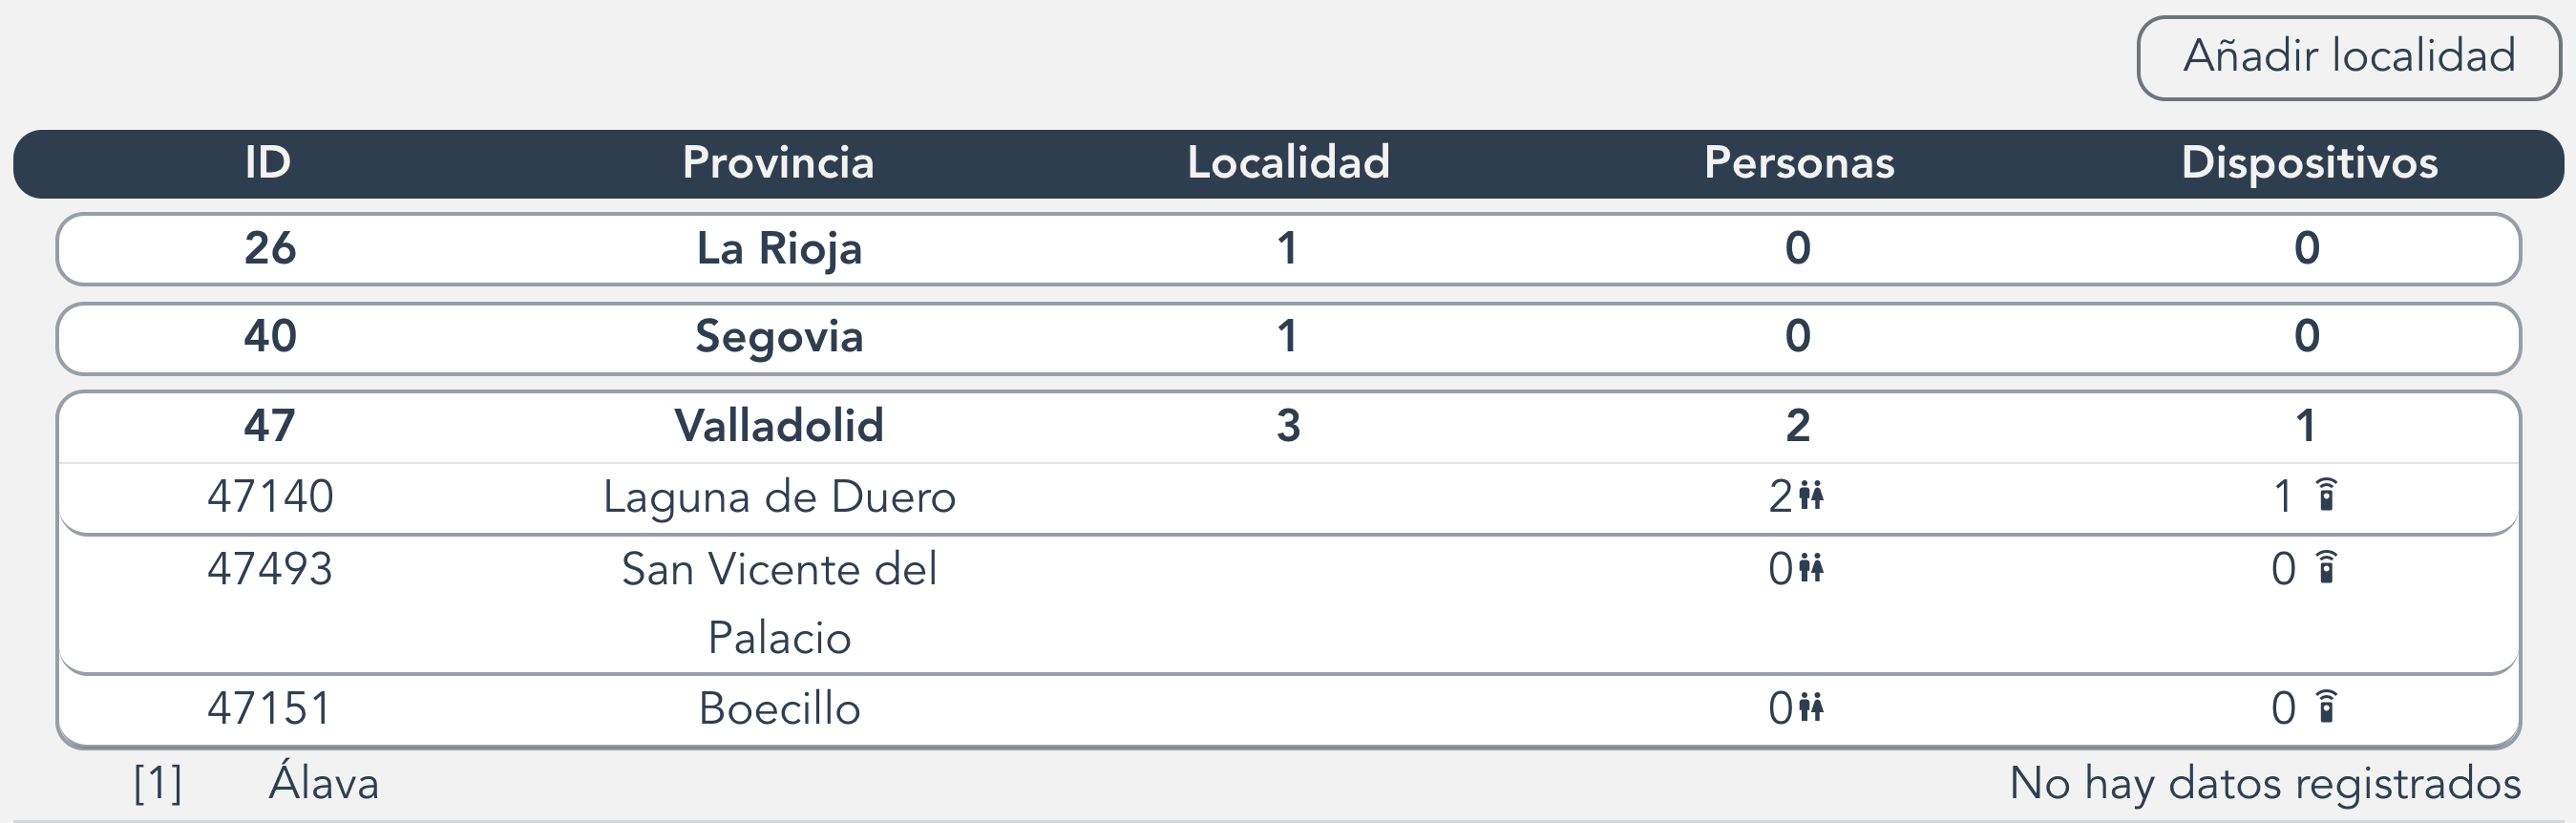
\includegraphics[width=11cm]{./img/web2/locations.table.opened.png}
        \caption{Localidades - Diseño final de lista: despliegue de provincia.}
        \label{fig:web.dir}
    \end{figure}
    
    En cuanto al diseño final se puede apreciar la posibilidad de añadir nuevas localidades. Para ello se planteó la posibilidad de añadirlo vía formulario: nombre de la localidad, código postal, provincia, y posición geográfica.
    
    \begin{figure}[H]   
        \centering
        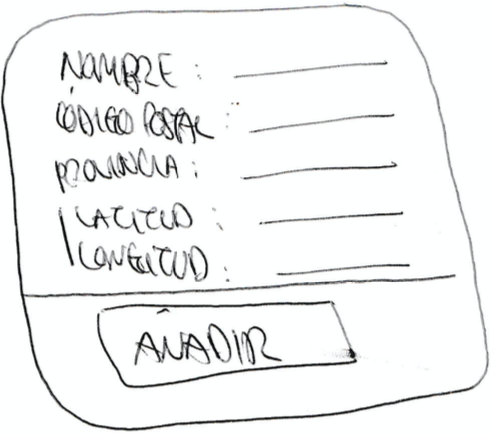
\includegraphics[width=6cm]{./img/web/locations/locations.add.pre.png}
        \caption{Localidades - Planteamiento de diseño para añadir nueva localidad.}
        \label{fig:location.add.post}
    \end{figure}
    
    Este prediseño, se ve que no es muy útil ya que la posición geográfica tendríamos que buscarla en otros servicios de mapas, o por que se debería introducir demasiados datos. 
    
    Finalmente se rediseñó, cambiando este prediseño por la implementación de un mapa que permitiese la búsqueda de la localidad, y añadirla seleccionándola en el mapa, de tal manera que se guarden todos los datos del formulario automáticamente sin necesidad de rellenarlos a mano, mejorando la experiencia de usuario.
    
    \begin{figure}[H]   
        \centering
        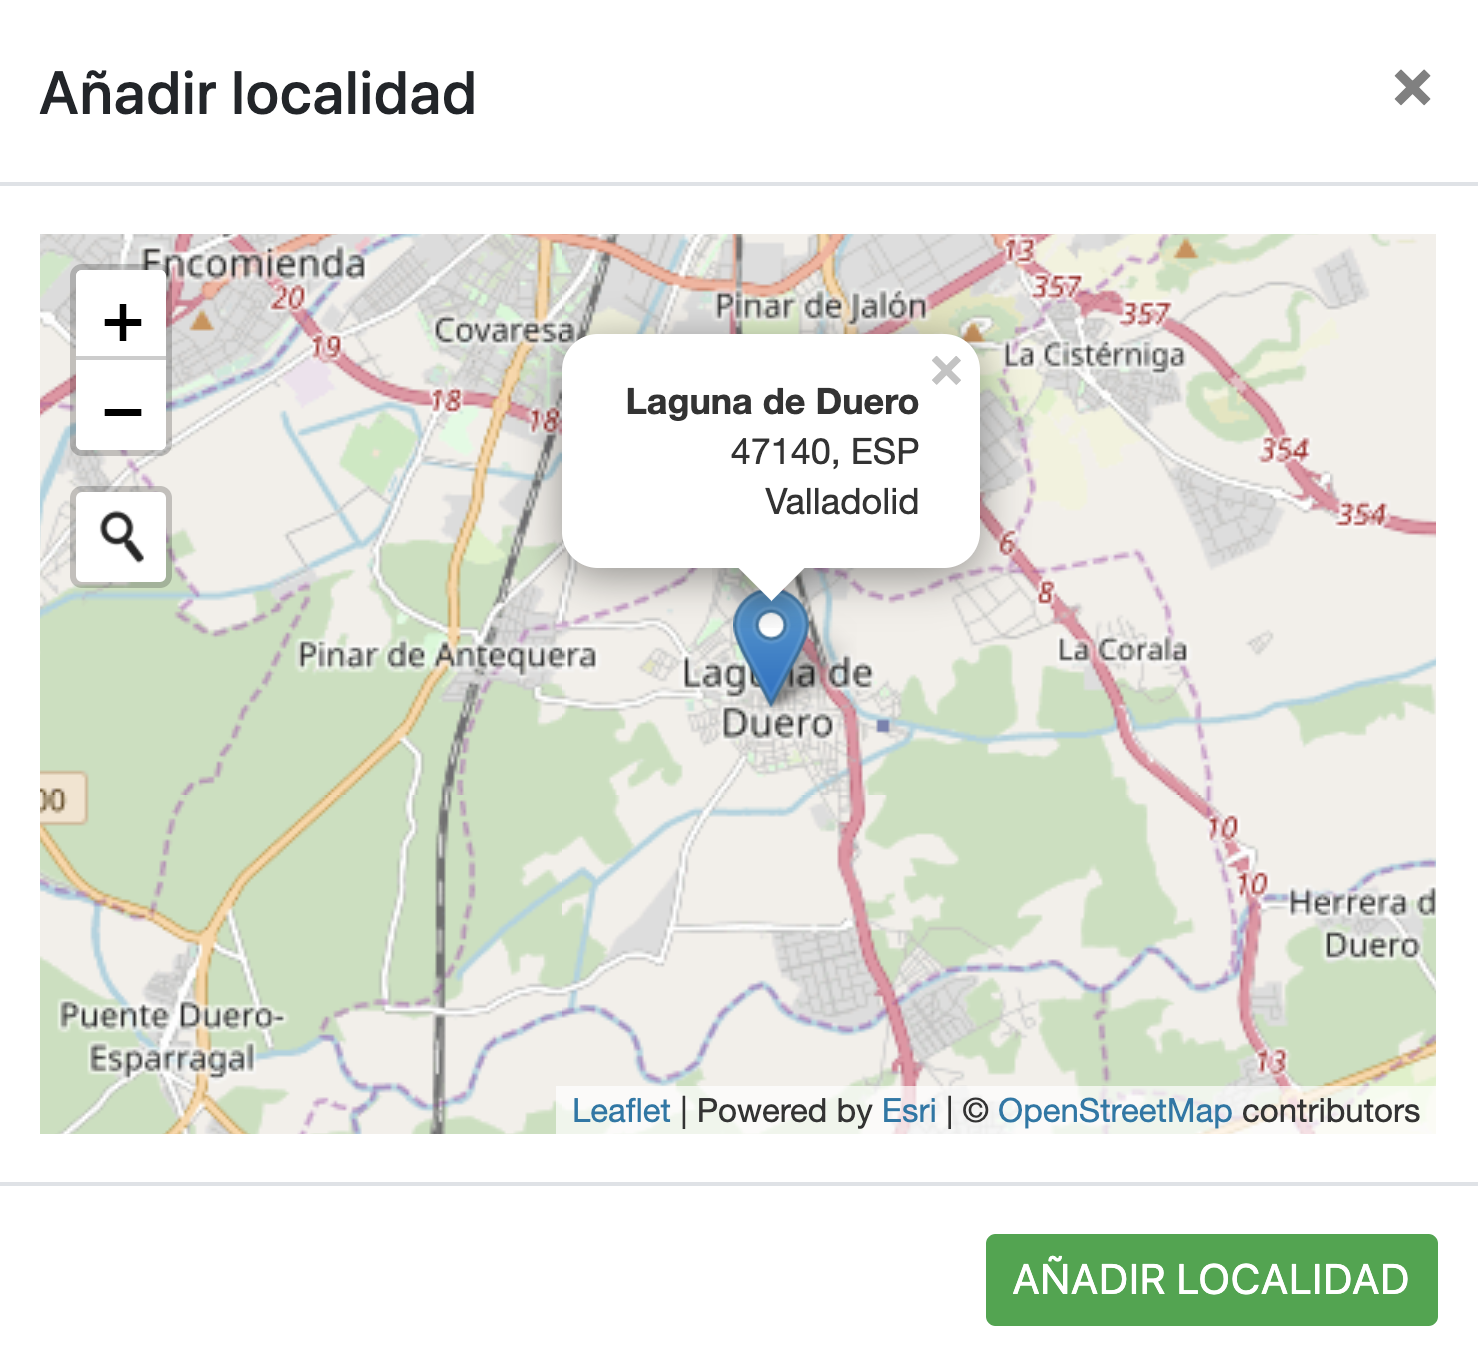
\includegraphics[width=8cm]{./img/web2/locations.add.map.png}
        \caption{Localidades - Diseño final de añadir nueva localidad.}
        \label{fig:location.add.post}
    \end{figure}
    
    En cuanto a la lista de localidades desplegada, un click sobre una localidad específica nos debería llevar al panel de configuraciones, permitiendo cambiar también la configuración de esa localidad.
    
    \item \textbf{Settings} %%% SETTINGS
    
    En esta sección se permite cambiar las configuracion prestablecida global. En caso de que se acceda a través de un enlace de una localidad, se permitirá cambiar la configuración de esa localidad, y en caso de acceder desde un dispositivo, se permitirá cambiar tango la global, como la del dispositivo, como la del pueblo del usuario asignado, en caso de que lo tenga.
    
    \begin{figure}[H]   
        \centering
        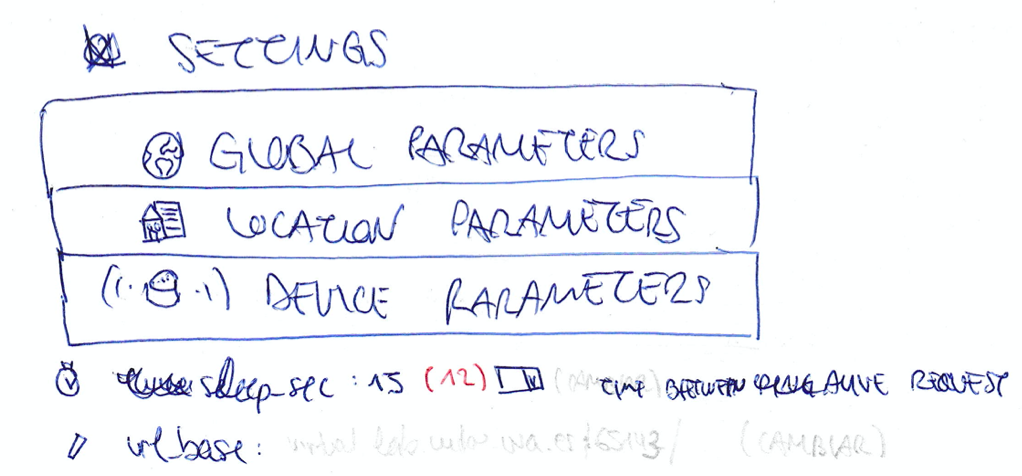
\includegraphics[width=10cm]{./img/web/settings/settings.pre.png}
        \caption{Settings - Planteamiento de diseño de configuraciones.}
        \label{fig:set.pre}
    \end{figure}
    
    De este planteamiento de diseño se han podido sacar aspectos interesantes, como la posibilidad de mostrar la configuración específica de un dispositivo, o si tiene aún alguna configuración pendiente específica por instalar mostrando esos valores pendientes en rojo al lado del valor que tiene instalado.
    
    En cuanto a la implementación real, se muestra cómo solo se ha definido al configuración de tiempo entre avisos, pudiendo ser esta parametrización fácilmente ampliable añadiendo simplemente nuevos campos, ya que la base y la lógica ya está montada.
    
    \begin{figure}[H]   
        \centering
        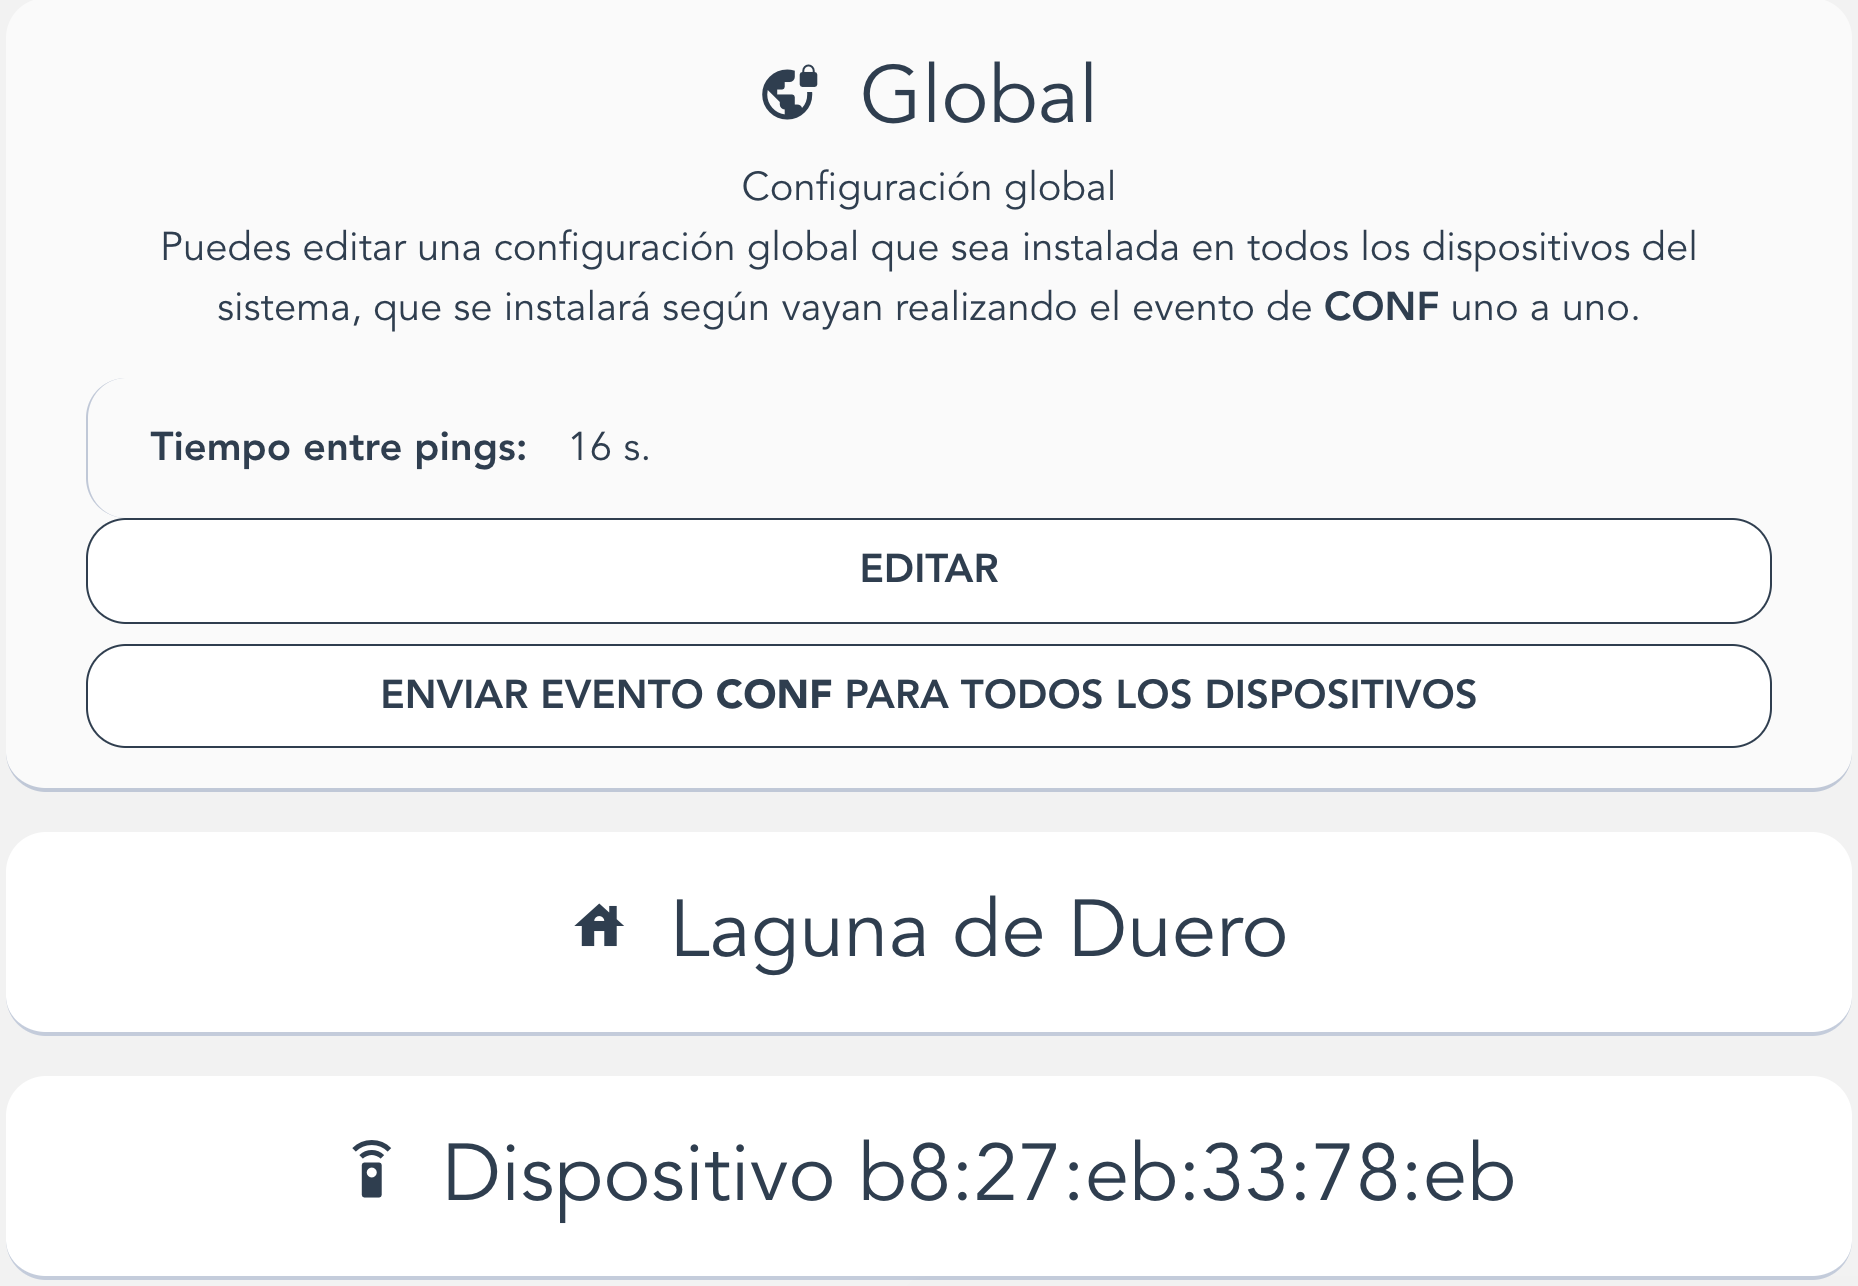
\includegraphics[width=10cm]{./img/web2/settings.global.png}
        \caption{Settings - Diseño final de configuración global.}
        \label{fig:set.global}
    \end{figure}
    
    \begin{figure}[H]   
        \centering
        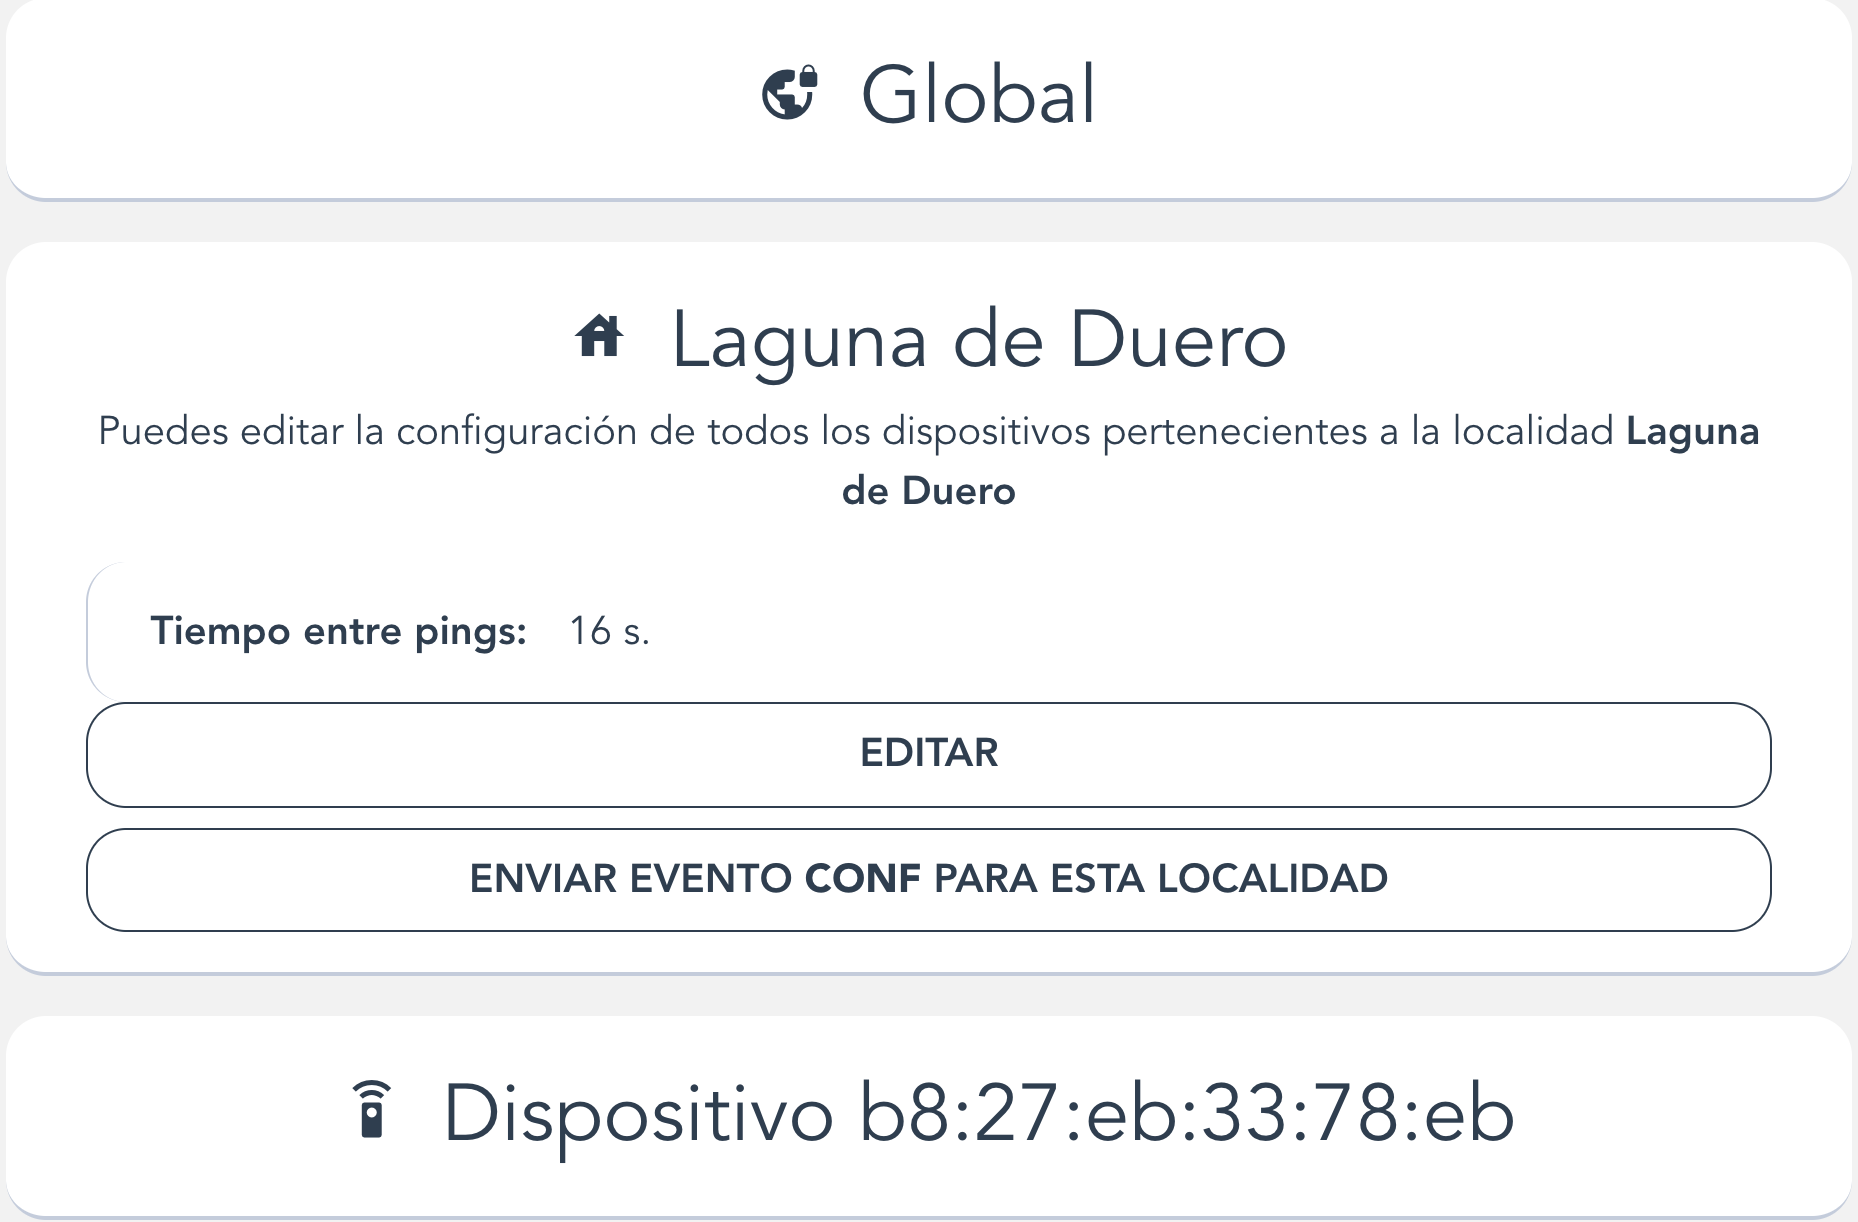
\includegraphics[width=10cm]{./img/web2/settings.location.png}
        \caption{Settings - Diseño final de configuración local.}
        \label{fig:set.local}
    \end{figure}
    
    \begin{figure}[H]   
        \centering
        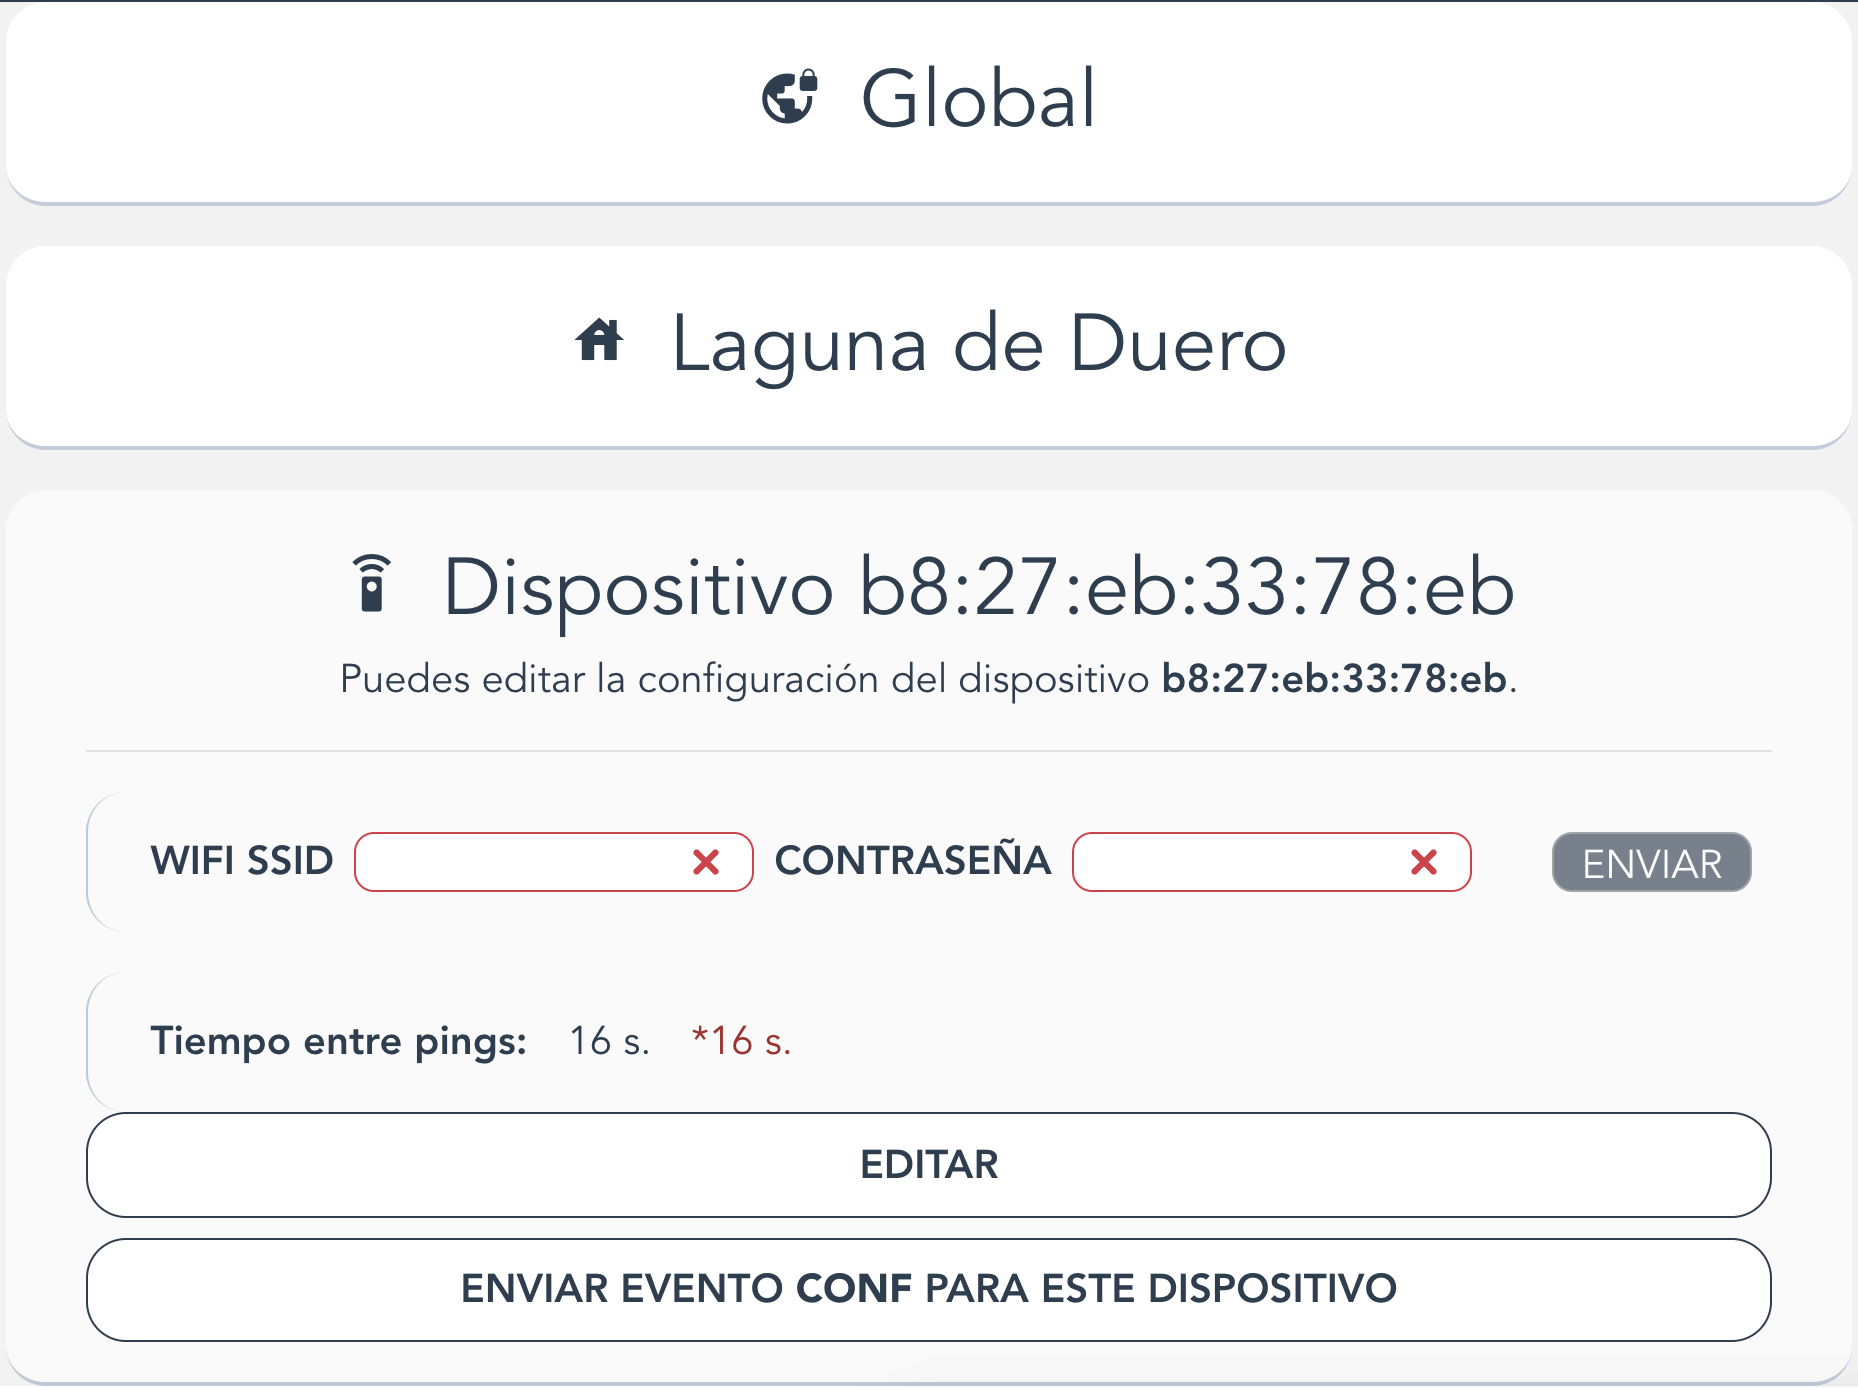
\includegraphics[width=10cm]{./img/web2/settings.device.png}
        \caption{Settings - Diseño final de configuración de un dispositivo.}
        \label{fig:set.device}
    \end{figure}
    
    
    \item \textbf{Usuarios} %%% USUARIOS
    
    Se mostrará una lista simple de todos los usuarios almacenados, de tal manera que aparezcan sus datos básicos, al igual que aparecerá su dispositivo asociado.
    La lista se debería poder filtrar en funcion del nombre, dni o dispositivo asociado con el fin de poder encontrar más fácilmente el usuario que se requiera.
    
    \begin{figure}[H]   
        \centering
        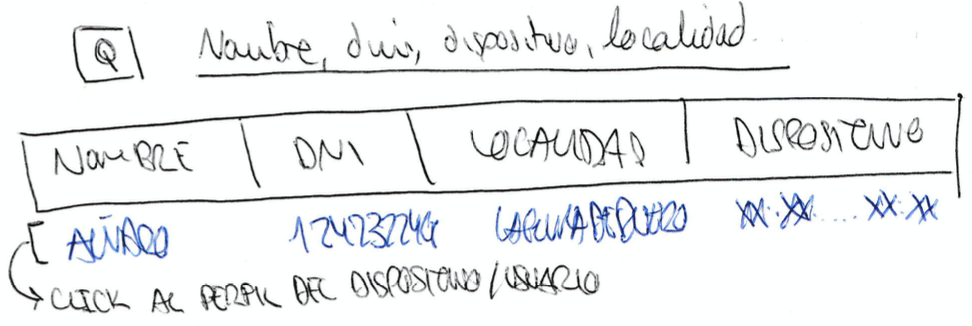
\includegraphics[width=10cm]{./img/web/users/users.pre.png}
        \caption{Users - Planteamiento de diseño de tabla de usuarios.}
        \label{fig:users.pre}
    \end{figure}
    
    \begin{figure}[H]   
        \centering
        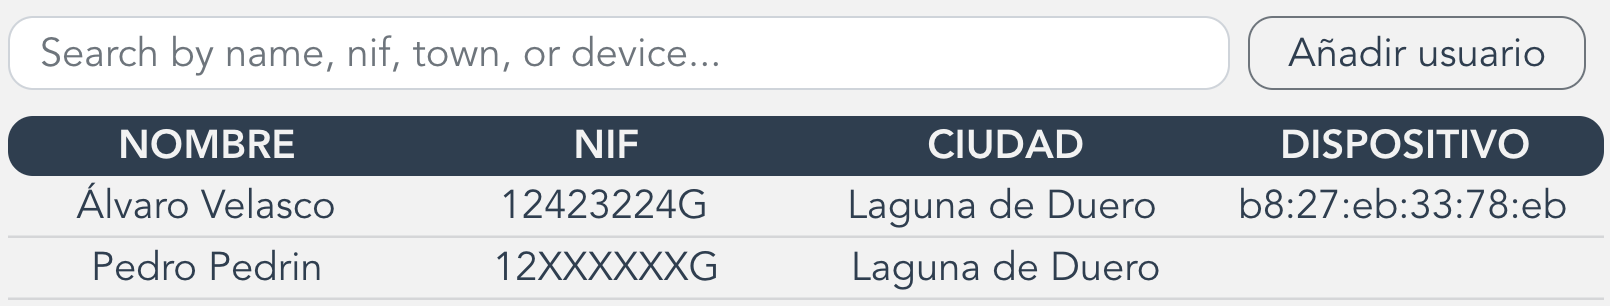
\includegraphics[width=11cm]{./img/web2/users.table.png}
        \caption{Users - Diseño final de tabla de usuarios.}
        \label{fig:users.post}
    \end{figure}
    
    También se debe dar la posibilidad de añadir usuarios nuevos al sistema, por lo que se realiza el diseño de un panel para añadir a los usuarios.
    
    \begin{figure}[H]   
        \centering
        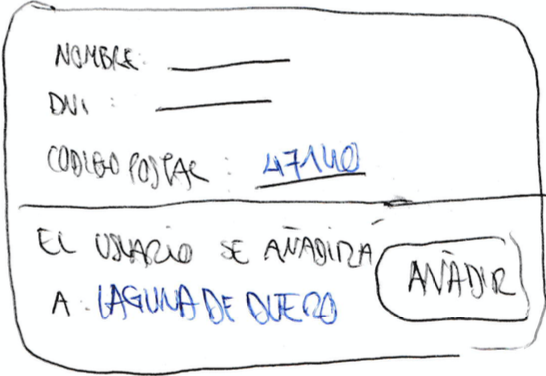
\includegraphics[width=6cm]{./img/web/users/users.add.pre.png}
        \caption{Users - Plantemiento de diseño de registro de usuarios}
        \label{fig:users.add.pre}
    \end{figure}
    
    A la hora de añadir usuarios, el código postal debe corresponder con el código postal de alguna ciudad ya registrada en el sistema, por lo que con tan solo ponerlo, ya te dice a qué localidad corresponde, si no, la aplicación web debería avisar sobre la necesidad de registrar anteriormente la localidad.
    
    \begin{figure}[H]   
        \centering
        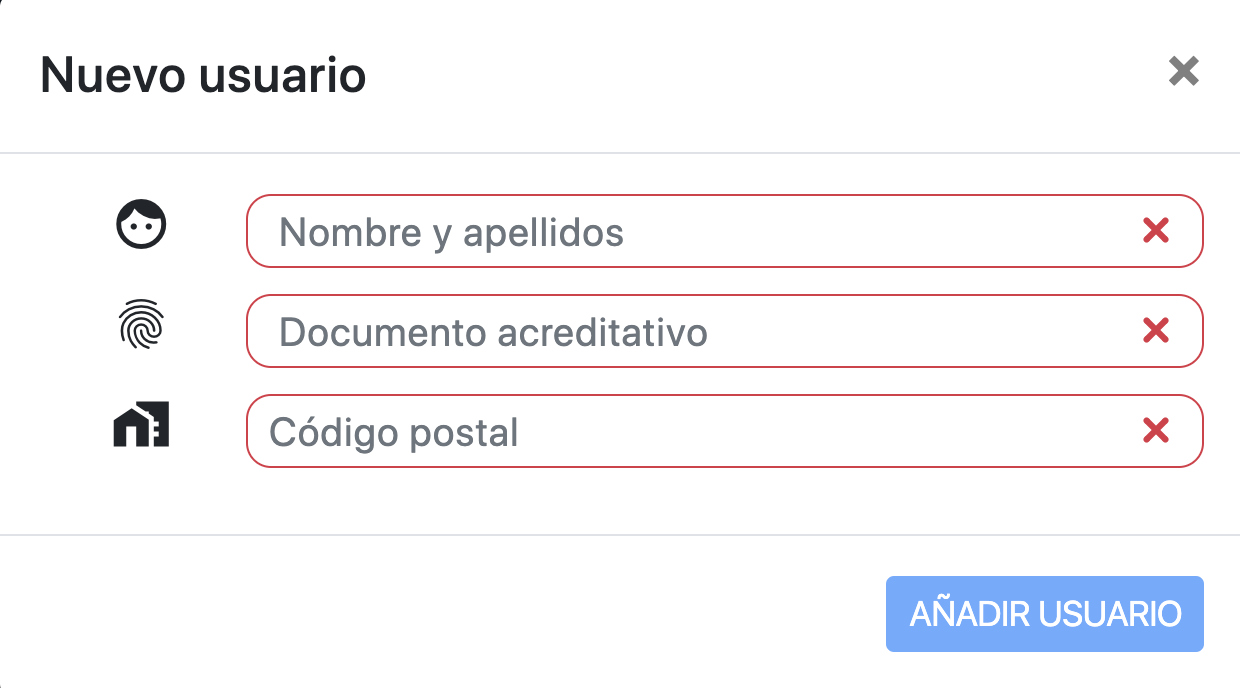
\includegraphics[width=10cm]{./img/web2/users.add.png}
        \caption{Users - Diseño final de registro de usuarios: código postal no registrado}
        \label{fig:users.add.fail}
    \end{figure}
        
    \begin{figure}[H]   
        \centering
        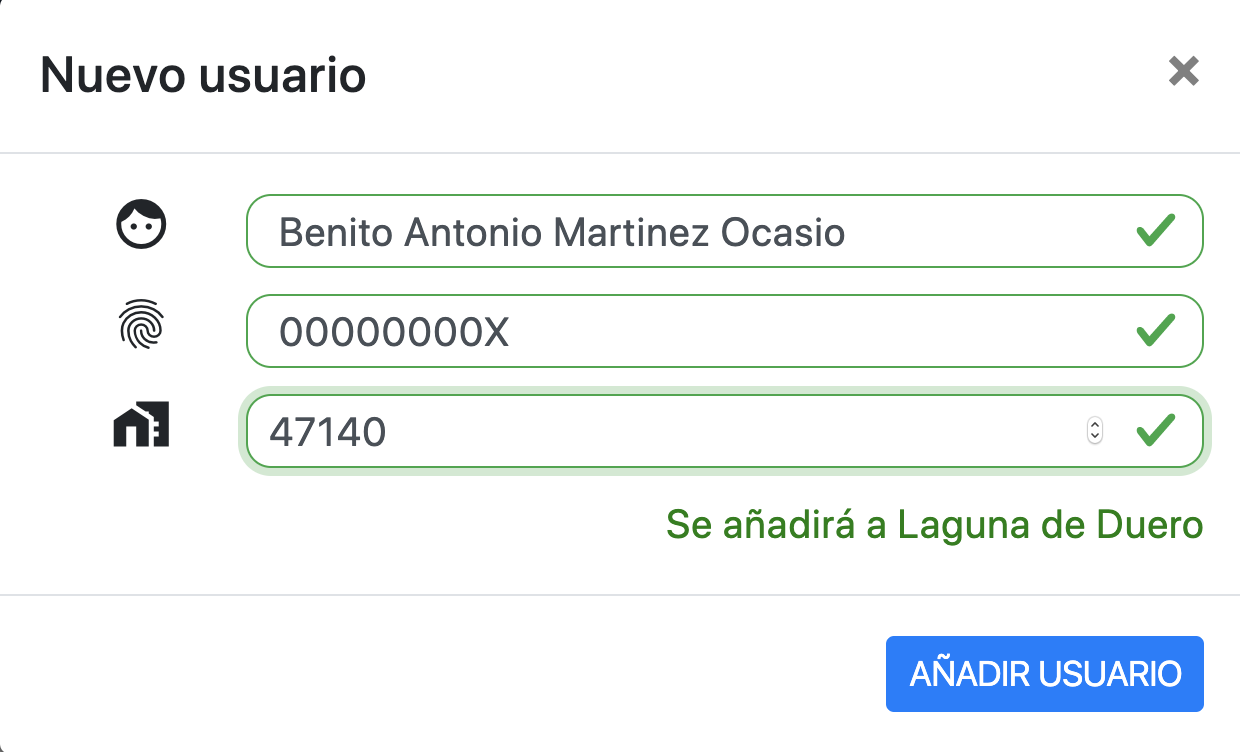
\includegraphics[width=10cm]{./img/web2/users.add.complete.png}
        \caption{Users - Diseño final de registro de usuarios}
        \label{fig:users.add.post}
    \end{figure}
        
    \item \textbf{Mapa} %%% USUARIOS
    
    La visualización a nivel estatal de la localización puede ser un buen aspecto para el control de los dispositivos, de modo que se pueda obsevar geográficamente cuántos dispositivos hay, y cómo están de dispersos por toda la geografía.
    
    Para ello se quiere poder mostrar un mapa donde aparezca un icono ubicado en la localización del usuario que lo tiene asignado, por lo que se necesita el diseño de ese icono:

    \begin{figure}[H]   
        \centering
        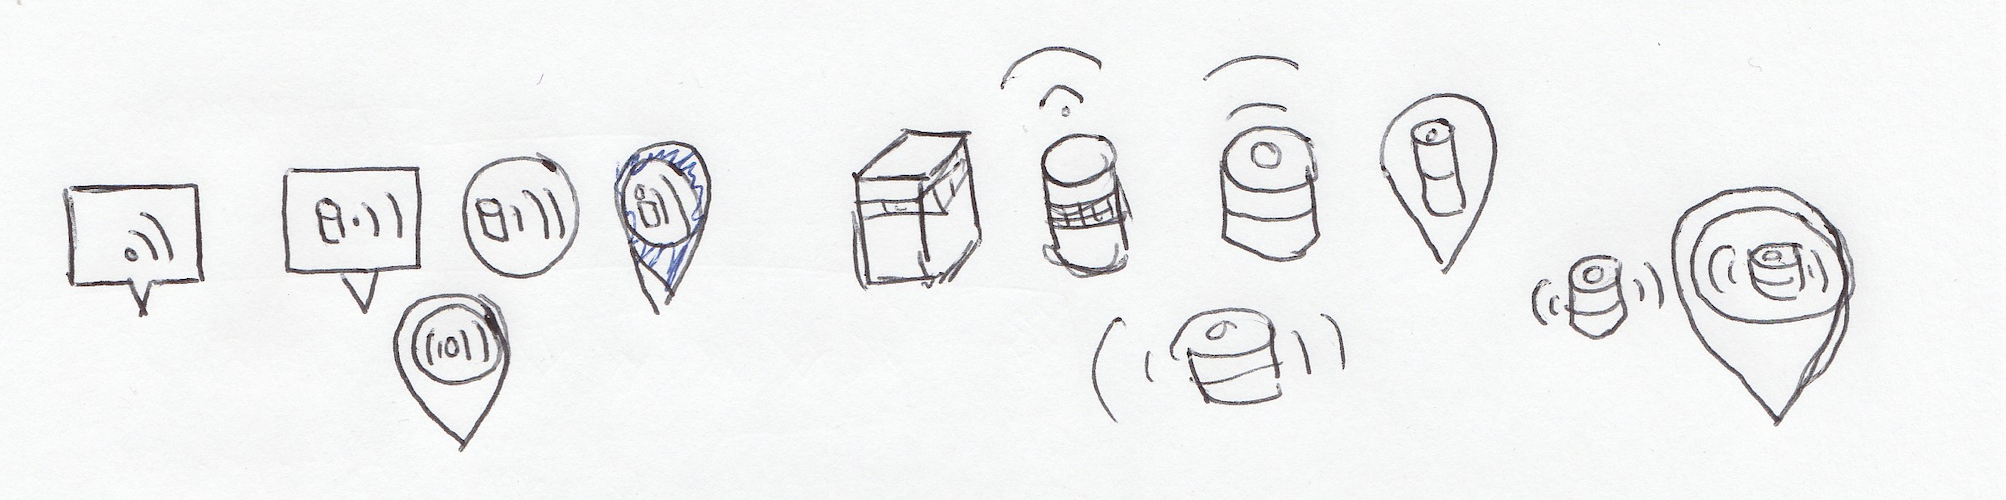
\includegraphics[width=13cm]{./img/icon/maps.icons.png}
        \caption{Mapa - Prototipo de iconos}
        \label{fig:icon.pre}
    \end{figure}

    El icono deberá aparecer en el mapa de color verde y ubicado en su lugar en caso de que el dispositivo esté asignado a algún usuario. En caso de que no tenga ninguna asignación, aparecerá en color amarillo, ubicado en la costa atlántica.
    
    \begin{figure}[H]   
        \centering
        
\includegraphics[width=3cm]{./img/icon/marker-green.png}
        \caption{Mapa - Marker de dispositivo asignado}
        \label{fig:icon.green}
    \end{figure}
    
    \begin{figure}[H]   
        \centering
        
\includegraphics[width=3cm]{./img/icon/marker-yellow.png}
        \caption{Mapa - Marker de dispositivo no asignado}
        \label{fig:icon.yellow}
    \end{figure}
    
    \begin{figure}[H]   
        \centering
        \includegraphics[width=11cm]{./img/web2/map.unassigned.png}
        \caption{Mapa - Diseño final: dispositivos separados}
        \label{fig:icon.yellow}
    \end{figure}
    
    En cuanto a los dispositivos mostrados en el mapa, se requiere que sean agrupados por localidades, mostrando el número en caso de que haya más de uno facilitando la representación y el número de ellos, como se ve en la figura \ref{fig:map.icon.grouped}, ya que mostrar todas las etiquetas juntas sería un problema de visualización. En caso de que se quiera conocer cuales son los dispositivos de la localidad, con tan solo dar click al número se acercaría el mapa y mostraría todos los markers sin solaparse, colocados en espiral y permitiendo, por tanto, la selección individual de cada uno de ellos.
    
        \begin{figure}[H]   
        \centering
        \includegraphics[width=11cm]{./img/web2/map.together.png}
        \caption{Mapa - Diseño final: agrupados por localidades}
        \label{fig:map.icon.grouped}
    \end{figure}
        
    \item \textbf{Perfil} %%% USUARIOS
    
    Las estadísiticas a mostrar en el perfil pueden ser tanto de un dispositivo sin asignar, como de un dispositivo asignado, como de un usuario sin dispositivo asignado.
    
    Debido a estas tres variantes se debe configurar la página de modo que permita ver ciertas funciones, ocultando otras, en función de qué es lo que se está observando.
    
    \begin{enumerate}
        
        \item Usuario sin dipositivo:
        Debe mostrar únicamente la información básica personal del usuario, y dar la posibilidad de asignar un dispositivo.
        
        \begin{figure}[H]   
            \centering
            \includegraphics[width=8cm]{./img/web/perfil/stats.user.device.png}
            \caption{Perfil - Planteamiento de diseño de perfil de usuario/dispositivo}
            \label{fig:testfigura}
        \end{figure}
        El diseño final de esta variante puede verse en la figura \ref{fig:perfil.userlibre.post}.
        
        \item Dispositivo sin asignar:
        Debe permitir ver tanto las estadísticas globales de actividad, como las tareas realizadas, pendientes, y asignar nuevas tareas. Se hace un diseño previo sobre como debería mostrarse la tarjeta con la información del usuario, con la posibilidad de asignar o desasignar un dispositivo.
        
        \begin{figure}[H]   
            \centering
            \includegraphics[width=8cm]{./img/web/perfil/stats.1.png}
            \caption{Perfil - Planteamiento de diseño de perfil de dispositivo sin usuario}
            \label{fig:perfil.tareas}
        \end{figure}
        
        \item Dispositivo asignado a usuario:
        Debe permitir ver tanto las opciones anteriores, limitadas por la fecha en que empezó la asignación, al igual que la información del usuario asociado, permitiendo desasignar al usuario el dispositivo, y asociar uno nuevo.
        
        \begin{figure}[H]   
            \centering
            \includegraphics[width=7cm]{./img/web/perfil/device-all.pre.png}
            \caption{Perfil - Planteamiento de diseño de pagina}
            \label{fig:perfil.pag}
        \end{figure}
        
        En la figura \ref{fig:perfil.pag} se puede observar ya un diseño general de cómo será la vista de la página para todas las variantes, teniendo en cuenta las posibilidades que hemos nombrado anteriormente.
        En función del estado que se encuentre, se ocultaría el panel de usuario, o saldría la opción de asignar un nuevo dispositivo.
        También, este prediseño deja ver la colocación de todas las tarjetas, apareciendo la posibilidad de un diseño en el cual se pueda modificar la configuración o añadir tareas a realizar por el dispositivo, que solo estaría visible en caso de haberlo. 
        
        Una vez tratada la posibilidad de añadir tareas, la página debería facilitar la tarea de ver qué tareas se han realizado, o qué tareas hay pendientes, al igual que poder ver cómo ha interactuado el usuario con el dispositivo, o ver las estadísticas sobre cuál es la mayor cuestión con la que se interactúa con el dispositivo. Por ello, se plasta otra variante de diseño que permita todas estas funciones, como es representado en la figura \ref{fig:perfil.tareas2}
        
        \begin{figure}[H]   
            \centering
            \includegraphics[width=7cm]{./img/web/perfil/stats.pre.png}
            \caption{Perfil - Planteamiento de diseño estadísticas}
            \label{fig:perfil.tareas2}
        \end{figure}
    \end{enumerate}
    
    Con este prediseño que da pie al muestreo de las estadísticas, una función útil sería el filtrado de ellas por fechas, pudiendo ser ese filtrado por días específicos, por meses, o por años.
    En cuanto a la posición de los filtros de las estadísiticas, se establecerá en la parte superior de la página, favoreciendo la intuición del administrador, mostrando su prototipo en la figura \ref{fig:perfil.filter}, que finalmente se ha implementado tal cual se diseñó, como muestra la figura \ref{fig:perfil.filter.post}.
    \begin{figure}[H]   
        \centering
        \includegraphics[width=8cm]{./img/web/perfil/stats.filter.png}
        \caption{Perfil - Planteamiento de diseño de filtro.}
        \label{fig:perfil.filter}
    \end{figure}
    
    \begin{figure}[H]   
        \centering
        \includegraphics[width=12cm]{./img/web/perfil/filter.post.png}
        \caption{Perfil - Diseño final de filtro. (Posibilidades)}
        \label{fig:perfil.filter.post}
    \end{figure}
    
    Finalmente, debido a la gran variante de posibilidades y prediseños de la página, se ha optado por una conjunción de todos los prediseños, dando prioridad a mostrar las opciones por tarjetas que serán colocadas en orden de mayor a menor uso del administrador, facilitando el acceso a todas las funcionalidades posibles.
    
    \begin{figure}[H]   
        \centering
        \includegraphics[width=12cm]{./img/web/perfil/stats.no-intents.png}
        \caption{Perfil - Diseño final del perfil: Usuario con dispositivo}
        \label{fig:perfil.dispositivoasignado.post}
    \end{figure}
    
    \begin{figure}[H]   
        \centering
        \includegraphics[width=12cm]{./img/web/perfil/stats.device.no-user.png}
        \caption{Perfil - Diseño final del perfil: Dispositivo libre}
        \label{fig:perfil.dispositivolibre.post}
    \end{figure}

    \begin{figure}[H]   
        \centering
        \includegraphics[width=12cm]{./img/web/perfil/stats.user.no-device.png}
        \caption{Perfil - Diseño final del perfil: Usuario libre}
        \label{fig:perfil.userlibre.post}
    \end{figure}
    
    Visto ya todo el sistema web, vemos que existe la posibilidad de asignar un dispositivo a un usuario específico, pero no se muestra como es esa asignación. Para ello, y pensando priorizar la usabilidad, se potencia mostrar una lista de los dispositivos que están disponibles, es decir, que no tienen ningún usuario asociado todavía. Esos dispositivos deberían estar apagados y amontonados en cajas en el despacho del administrador del proyecto. Por ello, y planteando lo que el administrador haría, sería conectar un dispositivo sin asignar, para ver que funciona. Por tanto, en la página, al mostrar los dispositivos sin asignar se ordenan poniendo los primeros los que han realizado un \textit{ping} de manera más reciente, ya que sería el que el administrador acabase de encender, como se muestra el prediseño en la figura \ref{fig:perfil.asign-device.pre}.
    
    \begin{figure}[H]   
        \centering
        \includegraphics[width=5cm]{./img/web/perfil/stats.assign.png}
        \caption{Perfil - Pranteamiento de diseño de asignación de dispositivo}
        \label{fig:perfil.asign-device.pre}
    \end{figure}
    
    En el diseño final, mostrado en la figura \ref{fig:perfil.asign-device.post} no se realiza ningún cambio de diseño, dando por bueno y correcto el diseño previo.
    
    \begin{figure}[H]   
        \centering
        \includegraphics[width=9cm]{./img/web2/profile.add.device.png}
        \caption{Perfil - Diseño final de asignación de dispositivo}
        \label{fig:perfil.asign-device.post}
    \end{figure}
    
    En cuanto a las estadísticas sobre la actividad del usuario con el dispositivo, se ha optado por la opción de mostrar de base dos gráficas para las estadísticas:
    \begin{enumerate}
        \item Doughnut Chart: Para visualizar la relación entre la utilización de las distintas consultas.
        \item Gráfico de barras: Para visualizar a qué horas el dispositivo ha sido utilizado más veces. Esta gráfica puede ayudarnos en un futuro para ver en qué habitos del día a día se puede mejorar la experiencia del usuario.
    \end{enumerate}
    
    \begin{figure}[H]   
        \centering
        \includegraphics[width=12cm]{./img/web2/profile.stats.png}
        \caption{Perfil - Diseño final de consultas}
        \label{fig:perfil.consult.post}
    \end{figure}

    En caso de que se sospeche sobre un posible peligro acontecido en el hogar de nuestro usuario, se puede seleccionar la opción de \textit{Mostrar más información}, desplegando una tabla de color azul en la cuál aparecen las últimas 5 consultas que se han hecho al dispositivo, pudiendo identificar una consulta de auxilio, por ejemplo.
    
    Si se quiere más información sobre la información intercambiada en una consulta concreta se puede pulsar en la fila correspondiente, haciendo aparecer una segunda tabla en la cual se muestra la información relativa a esa consulta.
    
    \begin{figure}[H]   
        \centering
        \includegraphics[width=12cm]{./img/web2/profile.stats.opened.png}
        \caption{Perfil - Diseño final consultas: Ampliado}
        \label{fig:perfil.consult.plus}
    \end{figure}
\end{enumerate}

    Como se puede observar en la figura \ref{fig:perfil.dispositivoasignado.post}, la vista, en caso de tener un dispositivo asignado, o ser una vista referida a la configuración de un dispositivo, que también se puede ver en la figura \ref{fig:perfil.dispositivolibre.post}, aparecen diferentes tarjetas, como de las últimas tareas realizadas que corresponde a las ordenadas por un administrador, o los últimos estados del dispositivo, donde se podrá ver si el dispositivo ha estado en uso, o simplemente está conectado \textit{(ALIVE)}, lo cual puede ayudar a la identificación de su uso de manera más rápida para el administrador.
    
    Otras tarjetas que se pueden ver son la de añadir una nueva tarea al dispositivo, donde se podría por ejemplo solicitar su actualización o apagado de manera remota. Una vez que se seleccionase una de estas tareas para realizarse, aparecerían en la tarjeta vecina, en la lista de tareas pendientes.
    
    Esta otra vista permite ver tanto las pendientes, como acceder a la configuración del dispositivo, que sería la figura \ref{fig:set.device}.

%\newpage
%\section{Casos de uso}
%\subsection{Diagrama de casos de uso}

\subsection{Definición de casos de uso}

\subsection{Matriz de aproximación con requisitos}

%\newpage
%\section{Diagramas de secuencia}
%\subsection{Diagrama de casos de uso}

\subsection{Definición de casos de uso}

\subsection{Matriz de aproximación con requisitos}

        


\chapter{Despliegue}\label{cap.deploy}

En el presente capítulo se explicará los métodos por los cuales se debería poder desplegar todo el sistema de manera que podría dejarse una copia operativa que permitiese el control remoto de dispositivos asistentes.

\section{Introducción}

    Para que el sistema no presente fallos, una recomendación es el despliegue por orden de las pautas aquí mostradas, aun que no debería ser problema el despliegue en cualquier otro orden.

    La recomendación del orden a seguir en la guía es la siguiente:
    
    \begin{enumerate}
    
        \item Despliegue del backend.
        
        \item Despliegue del frontend.
        
        \item Instalación del dispositivo.
        
    \end{enumerate}
\newpage
\section{Guía}
\subsection{ Despliegue del Back End}
    Para el despliegue correcto del Back End es necesario seguir las siguientes pautas por el orden que marca la guía:

\subsubsection{Instalación de la base de datos}
    Para la base de datos se utilizará PostgreSQL, como se ha nombrado en la sección \ref{postgresql}.
    Esta base de datos puede ser sustituida por cualquier otra, como puede ser MySQL, pero deberá ser una base de datos relacional.
    
    Para ello, nos conectamos desde la máquina la cual hará de servidor, y seguimos los pasos:
    \begin{enumerate}
        \item Se obtienen los certificados:
            \begin{lstlisting}[language=bash]
        $ sudo apt-get install wget ca-certificates
            \end{lstlisting}
        
        \item Se añade la clave de postgresql:
            \begin{lstlisting}[language=bash]
        $ wget --quiet -O - https://www.postgresql.org/media/keys/ACCC4CF8.asc | sudo apt-key add -
            \end{lstlisting}
        
        \item Se configura:
            \begin{lstlisting}[language=bash]
        $ sudo sh -c 'echo "deb http://apt.postgresql.org/pub/repos/apt/ `lsb_release -cs`-pgdg main" >> /etc/apt/sources.list.d/pgdg.list'
            \end{lstlisting}
            
        \item Se actualiza:
            \begin{lstlisting}[language=bash]
        $ sudo apt-get update
            \end{lstlisting}
            
        \item Se instala postgresql:
            \begin{lstlisting}[language=bash]
        $ sudo apt-get install postgresql postgresql-contrib
            \end{lstlisting}
            
        \item Se crea la base de datos:
        
            Para ello, nos conectamos al usuario de postgres
            \begin{lstlisting}[language=bash]
        $ sudo su - postgres
            \end{lstlisting}
            Y accedemos a postreSQL:
            \begin{lstlisting}[language=bash]
        $ psql
            \end{lstlisting}
            
            Una vez dentro, se crea la base de datos, que en este caso se va a llamar \textit{assistant}, a la que podemos acceder tecleando simplemente su nombre.
            La creación de las tablas se va a dejar a Kotlin y a su framework Exposed, para evitar fallos en algún tipo de dato o una mala relación de claves.
            \begin{lstlisting}[language=bash]
        postgres@psql> CREATE DATABASE assistant;
            \end{lstlisting}
            
            Con esto sería suficiente, pero para proporcionar seguridad se procede al cambio de contraseña del usuario de postgres:
            \begin{lstlisting}[language=bash]
        postgres@psql> ALTER USER postgres PASSWORD 'nueva_contraseña';
            \end{lstlisting}
            
    \end{enumerate}
    
    Es muy importante recordar la contraseña, ya que es necesario utilizarla posteriormente en el despliegue del backend para permitir su acceso. Para el despliegue temporal, la contraseña utilizada será: \textbf{cu4lquie.Rar}
    
    En este punto, la base de datos ya estaría disponible para la conexión desde dentro del servidor, localizándola en el \textbf{puerto 5432}.

\subsubsection{Configuración y despliegue del backend}

    Para su despliegue de prueba, únicamente es necesaria la localización del archivo \textbf{JAR} y su colocación dentro del servidor en el directorio \textit{/home/assistant/core}. Este paso no es relevante, pero es recomendable para una correcta localización del archivo, ya que los logs del sistema se almacenarán y archivarán en una carpeta contenedora de esa ruta, de modo que todo se tendría mejor ordenado.
    
    Una vez con el fichero en esa ruta, tan solo se tiene que acceder a ese directorio y ejecutar el archivo:
    \begin{lstlisting}[language=bash]
        $ cd /home/assistant/core
        $ java -jar assistant.core.jar
    \end{lstlisting}
    
    Desplegado de esta manera se podría visualizar los logs del sistema en tiempo real, pero con el impedimento de que no se podría cerrar la consola. Para evitar este problema, se puede ejecutar de la siguiente manera, ocultando las salidas con el comando \textbf{nohup} y estableciéndolo en segundo plano con el símbolo \textbf{\&}
        \begin{lstlisting}[language=bash]
        $ cd /home/assistant/core
        $ nohup java -jar assistant.core.jar &
    \end{lstlisting}
    
    En caso de querer finalizar la ejecucción, tan solo habría que finalizar el proceso. Para ello obtenemos la lista de procesos:
    
    \begin{lstlisting}[language=bash]
        $ ps -ef | grep java
    \end{lstlisting}
    
    Lo que nos mostraría la lista de procesos java ejecutados en la máquina, de donde se puede ver el número de proceso que corresponde a nuestro backend, y se eliminaría de la siguiente forma:

    \begin{lstlisting}[language=bash]
        $ kill -9 numerodeproceso
    \end{lstlisting}
    
    El acceso al sistema desplegado de prueba podría darse a través de las credenciales de un administrador, las cuales tendrían un usuario llamado \textbf{admin}, al que le corresponde la contraseña \textbf{seren0314}. 
    
    En caso de querer cambiar la configuración por defecto, o los datos de acceso a la base de datos como el usuario y contraseña que se ha mencionado al comienzo de la guía, se deberá cambiar los valores establecidos del proyecto, que estan configurados en el siguiente fichero:
    
    \textit{/src/controller/model/util/Credentials.kt}
    
    Una vez estos datos hayan sido actualizados, se deberá volver a formar el archivo JAR, por lo que nos ayudaremos de la herramienta de gradle, que será ejecutada desde dentro de la carpeta del repositorio:
    
    \begin{lstlisting}[language=bash]
        $ gradlew shadowJar
    \end{lstlisting}
    
    Tras este comando, se generará \textbf{assistant.core.jar}, el cual está localizado en \textit{./build/lib/}.
    
    Una vez el archivo JAR está generado, se repetirían los pasos descritos al principio de la sección donde se ha descrito la posibilidad de un despliegue de prueba.
    
    Una vez desplegado, será accesible a través del puerto 8082.
    
    
\subsection{ Despliegue del Front End}
    Como ya se ha mencionado en numerosas ocasiones, el front end está elaborado con VueJS, el cual está integrado con el módulo de pacquetes de Node, también conocido como \textbf{npm}.
Esto nos permite la compresión de la totalidad del proyecto en tan solo clases html, css y javascript, además de los archivos de recursos como pueden ser las imágenes.

Para la realización de esta compresión tan solo hay que acceder a la carpeta del repositorio y ejecutar:

    \begin{lstlisting}[language=bash]
        $ npm run build
    \end{lstlisting}
    
    Lo cual generará una carpeta en el mismo repositorio llamada \textbf{dist}.
    
    El despliegue del front end se realizará por tanto copiando el contenido de esta carpeta y pegándolo dentro del servidor apache, que en el caso habitual se encuentra en la siguiente ruta:
    
    \textit{/var/www/html}
    
    y siendo accesible por tanto a través del puerto 80 de la ubicación de nuestro servidor.
    
\subsection{ Instalación del Dispositivo}
    La instalación del software en el dispositivo podrá ser flasheando una imagen con el sistema operativo y el asistente ya cargado.

La guía por tanto, no entrará en ese apartado ino en la posibilidad de instalar el asistente en cualquier dispositivo que disponga de una arquitectura Unix.

Para ello, se introducirá el repositorio \textbf{assistant.task} en el dispositivo, dentro del directorio \text y aprovechando los scripts contenidos en él, se instalará todo lo necesario.

\begin{enumerate}
    \item Acceso al repositorio:
    
        \begin{lstlisting}[language=bash]
            $ cd /home/pi/assistant.task
        \end{lstlisting}
    
    \item Instalacción de dependencias
    
        \begin{lstlisting}[language=bash]
            $ sh requirements.sh
        \end{lstlisting}
    
\end{enumerate}

Tras la ejecución del script ya se instalan las dependencias requeridas y se configura el inicio automático del controlador remoto del asistente en cada reinicio de la máquina.



\newpage
\section{Trabajo futuro}
La elaboración de este proyecto deja abiertas las puertas a la elección e implementación final del asistente, ya que el presente documento narra la manera en la cual se ha implementado el controlador del dispositivo y cómo se puede manejar de manera remota un dispositivo, dejando sin implementar el asistente inteligente pero permitiendo la inclusión de cualquiera de los nombrados en el apartado \ref{mercato}, o cualquiera de los que serán creados en el futuro.

También, la manera de trabajar del controlador del dispositivo permite la inclusión sencilla de nuevas tareas, sin requerir la modificación de los archivos contenedores de las ya existentes.
 

%% escenarios


\appendix

%\chapter{Manual de Usuario}\label{aped.A}
%\input{./anexos/a1manual.tex}
%\chapter{Contenidos del CD-ROM}\label{aped.B}
%\input{./anexos/a2cdrom.tex}


\cleardoublepage
\addcontentsline{toc}{chapter}{Bibliografía}
\begin{thebibliography}{X}

\bibitem{nielsen}
\textsc{The Nielsen Company} (2018). \textit{Nielsen: Despite their bast capabilities, smart speakers are all about the music}.
\\Recuperado a 17 de Enero de 2020, \\de \href{https://www.nielsen.com/us/en/insights/article/2018/smart-speaking-my-language-despite-their-vast-capabilities-smart-speakers-all-about-the-music/}

\bibitem{lopd}
\textsc{BOE.es} (2019, Junio 25). \textit{Ley Orgánica 3/2018, de 5 de diciembre, de Protección de Datos Personales y garantía de los derechos digitales}.
\\Recuperado a 17 de Enero de 2020, \\de \href{https://www.boe.es/buscar/act.php?id=BOE-A-2018-16673}

\bibitem{top-asistentes} 
\textsc{Laboratorio de Periodismo Luca de Tena} (2019, Octubre 17). \textit{El 42\% de los usuarios de altavoces inteligentes en España escuchan noticias a través de ellos}.
\\Recuperado a 19 de Enero de 2020, \\de \href{https://laboratoriodeperiodismo.org/altavoces-inteligentes-espana-noticias/}

\bibitem{google-almacena} 
\textsc{20Minutos} (2016, Junio 5). \textit{Google graba y almacena tu voz: dónde puedes escucharla (y borrarla)}.
\\Recuperado a 17 de Enero de 2020, \\de \href{https://www.20minutos.es/noticia/2762528/0/google-graba-almacena-tu-voz-donde-como-borrarlo/}

\bibitem{escandalo-amazon} 
\textsc{Píxel, El Mundo}. (2019, Julio 4) \textit{Escándalo en Amazon: la empresa reconoce que guarda tus conversaciones para siempre}.
\\Recuperado a 19 de Enero de 2020, \\de \href{https://www.elmundo.es/tecnologia/2019/07/04/5d1ccf42fc6c833f3f8b460d.html}

\bibitem{mycroft-doc}
\textsc{Mycroft AI} (n.d.). \textit{Documentation}.
\\Recuperado a 20 de Enero de 2020, \\de \href{https://mycroft-ai.gitbook.io/docs/}

\bibitem{mycroft-com}
\textsc{Mycroft AI} (n.d.). \textit{Community}.
\\Recuperado a 20 de Enero de 2020, \\de \href{https://community.mycroft.ai/}

\bibitem{mod-it-inc} 
\textsc{ProyectosAgiles.com} (n.d.). \textit{Desarrollo iterativo e incremental}.
\\Recuperado a 22 de Enero de 2020, \\de \href{https://proyectosagiles.org/desarrollo-iterativo-incremental/}

\bibitem{ktor} 
\textsc{JetBrains}, (n.d.). \textit{Ktor Servers}
\\Recuperado a 18 de Enero de 2020, \\de \href{https://ktor.io/servers/index.html}

\bibitem{koin} 
\textsc{InsertKoinIO} (2019, Noviembre 5). \textit{Koin}.
\\Recuperado a 18 de Enero de 2020, \\de \href{https://github.com/InsertKoinIO/koin#readme}

\bibitem{oauth2} 
\textsc{OAuth.net} (n.d.). \textit{OAuth 2.0}
\\Recuperado a 18 de Enero de 2020, \\de \href{https://oauth.net/2/}

\bibitem{endpoint} 
\textsc{SmartBear.com} (n.d.). \textit{What is an API Endpoint?}
\\Recuperado a 18 de Enero de 2020, \\de \href{https://smartbear.com/learn/performance-monitoring/api-endpoints/}

\bibitem{myndocs.oauth2} 
\textsc{Myndocs} (2019, Septiembre 7). \textit{Kotlin OAuth2 server}.
\\Recuperado a 18 de Enero de 2020, \\de \href{https://github.com/myndocs/kotlin-oauth2-server}

\bibitem{exposedsql} 
\textsc{JetBrains} (2019, Junio 3). \textit{Exposed SQL DSL}.
\\Recuperado a 18 de Enero de 2020, \\de \href{https://github.com/JetBrains/Exposed}

\bibitem{jsoup} 
\textsc{Jonathan H.} (n.d.). \textit{Download and install JSoup}.
\\Recuperado a 19 de Enero de 2020, \\de \href{https://jsoup.org/download}

\bibitem{vue-curve}
\textsc{Ben R.} (2019, Diciembre 5). \textit{Vue vs React: Which is the Better Framework?}
\\Recuperado a 19 de Enero de 2020, \\de \href{https://buttercms.com/blog/vue-vs-react-which-is-the-better-framework}

\bibitem{bootstrap-vue} 
\textsc{Bootstrap-Vue} (n.d.). \textit{Components}.
\\Recuperado a 19 de Enero de 2020, \\de \href{https://bootstrap-vue.org/docs/components}

\bibitem{leaflet} 
\textsc{Leaflet}(n.d.). \textit{An open-source JavaScript library for mobile-friendly interactive maps}.
\\Recuperado a 19 de Enero de 2020, \\de \href{https://leafletjs.com/reference-1.6.0.html}

\bibitem{hxc} 
\textsc{Universidad de Valladolid} (n.d.). \textit{Preguntas Frecuentes}.
\\Recuperado a 21 de Enero de 2020, \\de \href{http://www.uva.es/export/sites/uva/2.docencia/2.02.mastersoficiales/2.02.13.preguntasfrecuentes/index.html}

\bibitem{salario-junior} 
\textsc{Indeed.com} (2019, Diciembre). \textit{Salarios para empleos de Programador/a junior en España}.
\\Recuperado a 21 de Enero de 2020, \\de \href{https://es.indeed.com/salaries/programador-junior-Salaries}

\bibitem{spm}  \\
\textsc{Bob Hughes and Mike Cotterell} (2009). \textit{Software Project Management}. McGraw-Hill Education.

\bibitem{mvvm} 
\textsc{Jeremy L.} (2014, Abril 24). \textit{Model-View-ViewModel (MVVM) Explained}.
\\Recuperado a 23 de Enero de 2020, \\de \href{https://www.wintellect.com/model-view-viewmodel-mvvm-explained/}

\bibitem{vuecomp} 
\textsc{Eder N.} (2017, Octubre 9). \textit{The Vue architecture that worked for me. (in small and large apps)}.
\\Recuperado a 23 de Enero de 2020, \\de \href{https://medium.com/@ederng/the-vue-architecture-that-worked-for-me-in-small-and-large-apps-9b253cf92951}

\bibitem{crontab} 
\textsc{Vivek G.} (2019, Julio 19). \textit{Linux Execute Cron Job After System Reboot}.
\\Recuperado a 24 de Enero de 2020, \\de \href{https://www.cyberciti.biz/faq/linux-execute-cron-job-after-system-reboot/}

\bibitem{clean-arch-book}
\textsc{Robert C. Martin} (2017). \textit{Clean Architecture: A Craftsman's Guide to Software Structure and Design}. Pearson.

\end{thebibliography}


\end{document}
